\chapter{Grundlagen und Methoden} 
In diesem Abschnitt werden die verwendeten Grundlagen und Methoden, die für die Umsetzung dieses Diplomarbeitsprojekts notwendig sind, dargestellt. Falls bei der Umsetzung mehrere Möglichkeiten zur Wahl standen, werden die einzelnen Möglichkeiten miteinander verglichen und nach einem Vergleich wird die besser geeignete Variante ausgewählt.


\section{Analyse des vorhandenen Systems}
Das bestehende System des Auftraggebers umfasst die Komponenten Grafana Server, Webserver und eine Datenbank mitsamt den notwendigen Algorithmen, um diese mit Echtzeitdaten zu befüllen. Bei der vorgegebenen Datenbank handelt es sich um einen MariaDB SQL-Server in der Version 10.1.48. Bei MySQL handelt es sich um eine quelloffene Implementierung des SQL Standards in der Version 5.0.12. In der nachfolgenden \autoref{fig:vorhandeneSystemAuftraggeber}  ist das vorhandene System des Auftraggebers ersichtlich.
\newline

\begin{figure}[h]
	\centering
	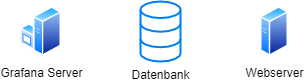
\includegraphics[height=2.5cm,width=8cm]{images/vorhandeneSystemAuftraggeber}
	\caption{ Vorhandene System des Auftraggebers}
	\label{fig:vorhandeneSystemAuftraggeber}
\end{figure}
Der Grafana Server wird übernommen, um Dashboards für die Energiesysteme und Panels für die Energietechnologien zu erstellen. Dabei können mehrere Statistiken, auch Panels genannt, zu einem Dashboard zusammengefasst werden, um somit eine Ordnerstruktur am Grafana Server zu erlangen. Der Webserver wird als Produktivserver benützt, um die fertige Website zu präsentieren. Die vorhandene Datenbank wird aufgrund deren Schemas nicht übernommen, stattdessen wird ein neues besseres Datenbankschema entwickelt. Die dafür notwendigen Algorithmen, um die neue Datenbank mit Echtzeitdaten zu befüllen, werden vom Auftraggeber entwickelt.



\subsection{Begriffe}
In diesem Abschnitt werden notwendige Begriffe, die in dieser Diplomarbeit eine wichtige Rolle spielen und zu Missverständnissen führen könnten, erklärt.

\subsubsection{Echtzeitdaten} \label{sec:Echtzeitdaten}
Der Begriff Echtzeitdaten ist definiert durch die regelmäßige und in gleichen Zeitabständen erfolgende Erfassung sowie Verarbeitung von Daten einer Energietechnologie. Der Zeitabstand der Datenerfassung bei den Energietechnologien beträgt 30 Sekunden. Aufgrund des vorgegebenen Zeitabstandes werden die Echtzeitdaten als weiche Echtzeitanforderung definiert, da das Produkt alle einkommenden Daten schnellstmöglich mit einem konstanten Zeitabstand von 30 Sekunden bearbeitet. Ein Überschreiten dieser Zeitgrenze wird nicht als Versagen definiert, solange sich die Zeit noch in einem akzeptablen Toleranzbereich von wenigen Sekunden befindet. Eine Unterschreitung der Zeitangabe ist sehr selten möglich.  


\subsubsection{Energietechnologie} \label{sec:Energietechnologie}
Als Energietechnologie wird ein Stromerzeuger, Stromverbraucher oder ein Energiespeicher bezeichnet. Stromerzeuger sind PV-Anlagen oder Windkraftanlagen. Stromverbraucher sind E-Ladestationen oder Hausanschlusszähler. Batteriespeicher oder Wärmespeicher sind Speicher-Energietechnologien. Die von diesen Technologien erfassten Echtzeitdaten werden in einer Datenbank gespeichert und anschließend grafisch in Form von Statistiken visualisiert.

Dabei werden folgende Echtzeitdaten für die Statistiken verwendet:

\begin{itemize}
	\item Erzeuger/Verbraucher - Leistung [kW]
	\item Erzeuger/Verbraucher - Energie [kW/h]
	\item Speicher – Kapazität/Temperatur [kW/h]/[°]
\end{itemize}

Die folgende Tabelle bietet eine Übersicht aller vorhandenen Energietechnologien.
In der ersten Spalte der Tabelle befinden sich reine Erzeuger-Energietechnologien[PM1] . Verbraucher-Energietechnologien sind in der zweiten Spalte ersichtlich. Speicher-Energietechnologien in der dritten Spalte und in der vierten und zugleich auch letzten Spalte befinden sich Energietechnologien, die sowohl als Verbraucher-Energietechnologie und als Erzeuger-Energietechnologie definiert sind.
\begin{table}[]
	\begin{tabular}{|l|l|l|l|}
		\hline
		\textbf{Erzeuger} &\textbf{Verbraucher}  & 	\textbf{Speicher}            &  \textbf{Verbraucher \& Erzeuger}           \\ \hline
		PV-Anlage                   & Wasserstoff- Elektrolyse    & Batteriespeicher     & Biomasseheizkraftwerk             \\ \hline
		Stromnetzbezug              & E-Ladestation               & Wasserstoff-speicher & Biomasseheizwerk                  \\ \hline
		Wasserstoff Brennstoffzelle & Hausanschlusszähler         & Wärmespeicher        & Biomassekessel                    \\ \hline
		Windkraftanlage             & Gebäude- Wärmebedarfszähler & Kältespeicher        & Kompressionskältemaschine         \\ \hline
		Wärmenetzbezug              & Gebäude- Kältebedarfszähler &                      & Ab- oder \newline \\ &&&Adsorptionskältemaschine \\ \hline
		Solarthermieanlage          &                             &                      &                                   \\ \hline
		Wärmepumpe                  &                             &                      &                                   \\ \hline
	\end{tabular}
\caption{Energietechnologien}
\label{tab:Energietechnologien}
\end{table}


\newpage
\subsubsection{Energiesystem} \label{sec:Energiesystem}
Der Begriff Energiesystem fasst mehrere Energietechnologien in einem bestimmten Gebiet, die genau einem Energiesystem zugeordnet sind, logisch zusammen. Ein Energiesystem kann somit eine Gemeinde, ein Gebäude oder ein einziger Haushalt mit mehreren Energietechnologien sein.


\subsubsection{Front-End} \label{sec:Front-End}
Der Begriff Front-End beschreibt die Weboberfläche auf welcher der Benutzer verschiedene Interaktionen durchführen kann. Dabei umfasst dieser Begriff alle Unterseiten der Weboberfläche welche von einem Benutzer verwendet werden können.


\subsubsection{Back-End} \label{sec:Back-End}
Mit dem Begriff Back-End ist das Laravel-Projekt, welches für die Ereignisse der Benutzer-Interaktionen zuständig ist, gemeint. Zusätzlich sind in diesem Begriff die Zugriffe auf die Datenbank sowie auf den Grafana Server mit eingebunden, welche durch das Laravel-Projekt durchgeführt werden.

\newpage
\section{Anforderungen an das Produkt}
Die Datenbank des Auftraggebers ist die größte Schwachstelle des vorhanden Systems.
Aufgrund dessen wird ein neues Datenbankschema entwickelt. Neben der Entwicklung eines neuen Datenbankschemas sind folgende Anforderungen an das Produkt gegeben:

\begin{itemize}
	\item Übersichtliche Darstellung von Energiesystemen und Energietechnologien auf einem Kartendienst
	\item Grafana-Statistiken mit Echtzeitdaten der Energietechnologien anzeigen
	\item Bildergalerie um Energietechnologien eines ausgewählten Energiesystems zu präsentieren
	\item Managementfunktion mit Hilfe von verschiedenen Benutzern für unterschiedliche Berechtigungen
\end{itemize}


\subsection{Schutz von vertraulichen Informationen}
Sämtliche Daten wie Adressen, Standorte (in Form von Koordinaten) oder die Namen der Ersteller von Energiesystemen oder Energietechnologien sind vertrauliche Informationen und sollten somit nicht für jeden einsehbar sein. Darum sind diese Daten nur in der Datenbank gespeichert, welche nur für Benutzer mit entsprechender Berechtigung zugänglich ist. Die Daten, die in den Grafana-Statistiken dargestellt werden, sind ebenso vertrauliche Daten. Die Informationen, die man einer solchen Statistik entnehmen kann, könnten in die falschen Hände gelangen und zu unerwünschten Tätigkeiten führen. Um dieses zu verhindern, sieht jeder angemeldete Benutzer nur seine eigenen Statistiken und keine anderen. Ein nicht angemeldeter Besucher sieht keine Statistiken.


\subsection{Statistische Auswertung}
Zur statistischen Auswertung wird das Daten visualisierungs Framework Grafana verwendet. In Grafana werden einzelne Energiesysteme als “Dashboards” abgebildet, in diesen Dashboards werden die Energietechnologien als “Panels” erstellt. In der Konfiguration der Panels werden die SQL Abfragen definiert aus welchen sich die Statistiken zusammensetzen. Die Statistiken bilden sowohl Echtzeit Daten als auch Daten der letzten 24 Stunden ab. Die Statistiken werden hier als Zeitreihen \footnote{ In diesen Diagrammen werden Zahlenwerte in Abhängigkeit von Zeitwerten angezeigt.	
 }. Diagramme abgebildet.


\newpage
\section{Architektur des Zielsystems}
Die \autoref{fig:Architektur} repräsentiert die Architektur des Zielsystems. Der Benutzer greift über die Weboberfläche auf den Webserver zu, wo sich das Laravel-Projekt befindet. Auf dieser Website kann der Benutzer verschiedene Interaktionen durchführen. Dabei ist die Weboberfläche ständig in Verbindung mit der Datenbank sowie dem Grafana Server. Sobald der Benutzer auf die Energiesysteme-Seite der Weboberfläche wechselt, wird eine Datenbankabfrage aller vorhandenen Energiesysteme durchgeführt. Zusätzlich dazu wird mittels API-Abfrage auf den Grafana Server zugegriffen, um Statistiken einer Energietechnologie anzuzeigen, falls dies vom Benutzer angefordert wird.

\begin{figure}[h]
	\centering
	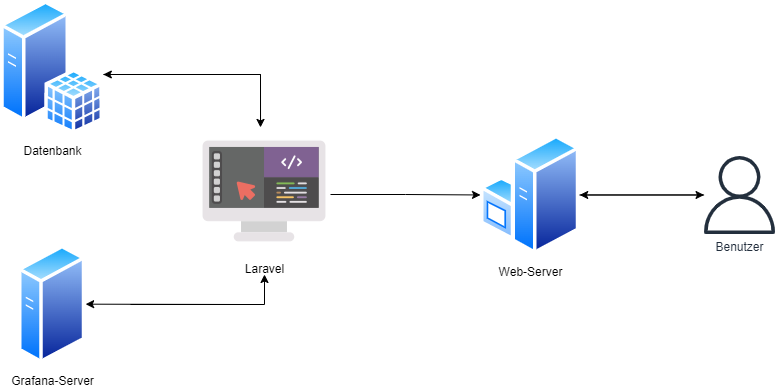
\includegraphics[height=7cm,width=15cm]{images/Architektur}
	\caption{Architektur des Zielsystems}
	\label{fig:Architektur}
\end{figure}

\subsection{Endgeräte}
Das Produkt wurde als Browser Anwendung entwickelt, um überall lauffähig zu sein. Es ist in Chrome, Firefox und Edge Browser getestet worden und ist dort voll funktionsfähig. Die Oberfläche wurde für einen 13 bis 27 Zoll Monitor entwickelt und funktioniert dort in jeder Zoomstufe einwandfrei. Klares Ziel war es, das Produkt nicht für den Mobiltelefongebrauch zu programmieren. Das Team hat sich bewusst gegen eine native Anwendungsentwicklung entschieden, um so die Verwendbarkeit auf allen Plattformen zu garantieren. Darüber hinaus würde eine parallele Anwendungsentwicklung auf den drei gängigen Betriebssystemen (Windows, MacOS, Linux) den zeitlichen Rahmen der Diplomarbeit sprengen. In welchen Browser Versionen das Produkt getestet wurde ist in der Tabelle \ref{tab:Browser und Versionen in denen das Produkt getestet wurde} ersichtlich. 

\newpage
\begin{table}[h]

	\begin{tabular}{|l|l|}
		\hline
		Browser & Version      \\ \hline
		Firefox & 99.0beta     \\ \hline
		Chrome  & 99.0.4844.51 \\ \hline
		Edge    & 99.0         \\ \hline
	\end{tabular}
\caption{Browser und Versionen in denen das Produkt getestet wurde}
\label{tab:Browser und Versionen in denen das Produkt getestet wurde}
\end{table}


\subsection{Serverseitig }
Bei PHP handelt es sich zum einen serverseitige zur Laufzeit interpretierte Skriptsprache, mit welcher sich Daten dynamisch auf Website anzeigen lassen. Da es sich bei Laravel um ein PHP Framework handelt, wird der Code am Webserver beim Laden der Website interpretiert. Laravel kommuniziert serverseitig mithilfe eines sogenannten ORM (Object Relational Mapper) mit der Datenbank. Hiermit kann der Programmierer auf vorgefertigte Funktionen des ORM zurückgreifen und muss Datenbankoperationen wie Abfragen oder das Erstellen von Tabelleneinträgen nicht als SQL Abfragen Formatieren.

\subsection{Clientseitige Interaktionen des Benutzers}
Bei dem Punkt Clientseitig befindet man sich in der Architektur des Zielsystems bei dem Element JavaScript und mit den damit verbundenen Interaktionen des Benutzers. Map-Interaktionen sind Interaktionen mit einer Karte, dazu gehört das Erstellen, Bearbeiten und Löschen von Energiesystemen sowie Energietechnologien. Eine weitere Interaktion wäre die Verwendung des Adresssuchfeldes, welche mit einem Klick auf den Button „Suche“ oder durch Drücken der Enter-Taste durchgeführt wird. Tabellen-Interaktionen sind eine zusätzliche clientseitige Aktion, da die vom DataTable\footnote{Eine genaue Begriffserklärung befindet sich in \ref{sec:DataTable}} bereitgestellten Funktionen wie die Suchfunktion, Sortierfunktion oder Seitennummerierung allesamt clientseitig stattfinden und somit keinen Einfluss auf das Back-End haben.
Folgende \autoref{fig:clientseitig}
 zeigt den Aufbau der einzelnen Elemente, die zusammenarbeiten, um die Website zu erstellen.


\begin{figure}[h]
	\centering
	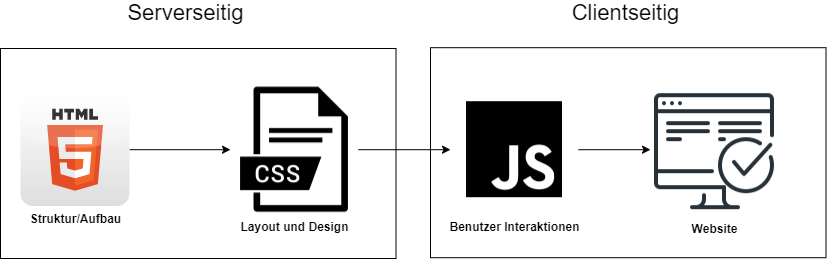
\includegraphics[height=4cm,width=12cm]{images/clientseitig}
	\caption{Clientseitiger Aufbau der einzelnen Elemente}
	\label{fig:clientseitig}
\end{figure}
\newpage
\subsection{Framework}
Die Wahl des Frameworks ist für die Umsetzung des Projekts entscheidend. Unter dem Begriff Framework versteht man eine Art Programmiergerüst, welches es dem Programmierer deutlich erleichtert, ein Produkt zu erstellen. Jedes Framework bietet spezielle Lösungen und Lösungsansätze an und damit hat jedes Einzelne sein eigenes Einsatzgebiet. Zusätzlich wurde noch die Software-Bibliothek React ergänzt, da auch diese eine mögliche Umsatzungsvariante ist. In den nachfolgenden Unterkapiteln werden mögliche Frameworks für die Umsetzung des Projekts kurz erklärt. In \ref{sec:Entscheidung des Frameworks} wird genauer darauf eingegangen, welches Framework gewählt wurde und aus welchem Grund.

\subsubsection{Laravel}
Das PHP-Framework Laravel, welches 2011 entwickelt wurde, basiert auf dem MVC Muster\footnote{wird in  \autoref{sec: MVC} genauer erläutert} und bietet damit eine sehr gute Strukturierung und Übersicht beim Arbeiten. Die meisten Projekte werden mit Laravel im Back-End in Kombination mit Vue.js im Front-End umgesetzt. Genauere Informationen zu Vue.js sind in \ref{sec: Vue.js} nachzulesen. Laravel bietet jedoch die Möglichkeit, im Back- als auch im Front-End verwendet zu werden. Es lässt sich in folgende Einzelteile strukturieren:

\begin{itemize}
	\item Migrations 
	\item Views
	\item Controller 
	\item Models
	\item Routen 
\end{itemize}

Migrations sind die Abbildung der Tabellenstruktur und ermöglichen es, bei richtiger .env Datei Konfiguration, mit artisan\footnote{artisan ist die in Laravel enthaltene Befehlszeilenschnittstelle} Befehlen, ganz einfach eine Datenbank und die dazugehörigen Tabellen zu erstellen und diese auch genauso einfach wieder zu löschen oder zu leeren. Views fungieren als visueller Gliederungspart zwischen den Controllern und den Benutzern. In ihnen wird alles, was auf der Oberfläche ersichtlich ist, ausprogrammiert und gestaltet. Controller bilden die Verbindung zwischen den Views und den Models und ermöglichen es dem Benutzer, Daten mithilfe eines Zugriffs auf das Model zu verändern. Models bilden die Datenstruktur ab und ermöglichen den Zugriff auf die Daten und die Änderung dieser. Routen vermitteln die Benutzerabfrage von der View mit dem dazugehörigen Controller und werden in der Datei “web.php” definiert. Der ganze Prozess ist in \autoref{fig:Laravel MVC} visuell dargestellt. 
\begin{figure}[h]
	\centering
	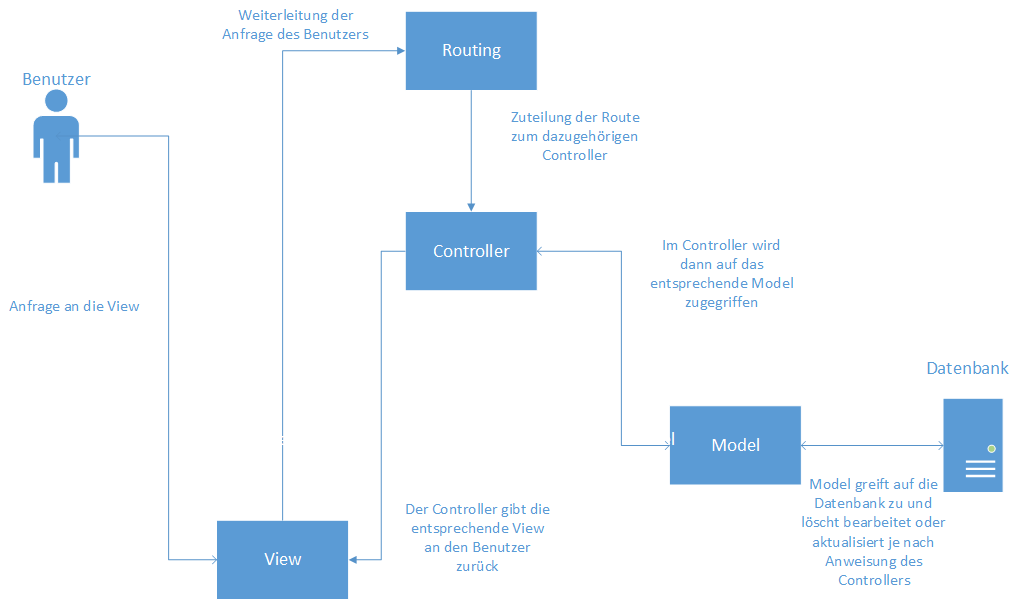
\includegraphics[height=8cm,width=15cm]{images/LaravelMVC}
	\caption{Laravel MVC}
	\label{fig:Laravel MVC}
\end{figure}
\newpage




\subsubsection{Angular}
Angular ist ein clientseitiges JavaScript-Web-Framework und wird meistens zum Erstellen von sogenannten Single Page Applications\footnote{Anwendung die nur auf einer Seite zu bedienen ist}, wie beispielsweise ein einfaches Bedienelement zur Steuerung einer Maschine, verwendet. Angular ist speziell für Web-, Desktop- und Mobile-Anwendungen entworfen. Ein weiterer Aspekt des Frameworks ist es, dass es von Google entwickelt wurde und so ein langfristiger Support gewährleistet ist. Angular macht es mit der Kombination aus HTML und TypeScript möglich, so ziemlich jede mögliche Aufgabenstellung zu bewältigen. Es bietet auch besondere Features wie eine bidirektionale Datenbindung an und ist somit gut für Echtzeitanwendungen geeignet. 
Alle Daten zu Angular wurden der Quelle \cite{Angular} entnommen.
\begin{figure}[h]
	\centering
	
\includegraphics[height=4cm,width=5cm]{images/Angular_Logo}
	\caption{Angular Logo}
	\label{fig:Angular Logo}
\end{figure}

\subsubsection{ASP.NET}
ASP.NET (Active Server Pages) ist ein Web Application Framework, welches 2002 von der Firma Microsoft veröffentlicht wurde. Es ist der Nachfolger des ASP Frameworks und bietet eine perfekte Grundlage, um dynamische Websites, Webanwendungen und Webservices zu entwickeln. Projekte werden hier in der Regel in der Sprache C\# programmiert. Jedoch besteht auch die Möglichkeit, andere Sprachen wie beispielsweise Perl, Python oder Cobol zu verwenden. ASP.NET bietet nicht nur die Möglichkeit, dynamische Websites zu erstellen, sondern auch Desktop Anwendungen.
Durch die vordefinierte Datenstruktur, die ASP.NET bereitstellt, hilft es dem Programmierer Programmiersprachen nicht zu vermischen und einen übersichtlichen Programmierstil beizubehalten. Des Weiteren können viele Teile automatisch generiert werden und ersparen dem Programmierer damit einen immensen Aufwand.

\begin{figure}[h]
	\centering
	
\includegraphics[height=4cm,width=7cm]{images/ASP.net_Logo}
	\caption{ASP.NET Logo}
	\label{fig:ASP.net Logo}
\end{figure}


Alle Informationen und Daten über ASP.NET können unter der Quelle xy (https://asp.mvc-tutorial.com/de/421/einfuhrung/was-ist-asp-net-mvc/) nachgelesen werden.

\subsubsection{React}
React ist eine JavaScript-Softwarebibliothek, die es erleichtert, Benutzeroberflächen in Form von Web Applikationen zu erstellen. Es ist komponentenbasiert, was bedeutet, dass jedes Element in Blöcken aufgebaut ist und durch Zusammenfügen dieser einzelnen Codebits kann dann eine sogenannte View erstellt werden. Dies bietet die Möglichkeit, bereits erstellte Codebits auch in anderen Views zu verwenden.\\ React wird oft zusammen mit ASP.NET verwendet.


Genaueres zu React kann unter der Quelle xy (https://t3n.de/news/react-facebook-623999/) nachgelesen werden.
\begin{figure}[h]
	\centering
	
\includegraphics[height=3cm,width=4cm]{images/React_Logo}
	\caption{React Logo}
	\label{fig:React Logo}
\end{figure}
\newpage

\subsubsection{Entscheidung des Frameworks}\label{sec:Entscheidung des Frameworks}
Positive und negative Aspekte jedes Framworks wurden vom Projektteam, mithilfe der Tabelle 2.3 abgewogen. Daten für diese Tabelle wurden aus den Quellen xy entnommen.

\begin{table}[h]
	
	
	\begin{tabular}{|l|l|l|}
		\hline
		\textbf{Framework} &
		\textbf{Vorteile} &
		\textbf{Nachteile }\\ \textbf{oder Bibliothek} && \\\hline
		React &
		\begin{tabular}[t]{@{}l@{}}Software Skalierbarkeit;\\ hohe Flexibilität;\\ Codebits ermöglichen es, \\die  Redundanz zu erhöhen; \\schnelles Rendering;\\ leichter Einstieg\end{tabular} &
		\begin{tabular}[t]{@{}l@{}}Es gibt nicht genug Möglichkeiten,\\ eine Webapp zu erstellen \\ und benötigt Zusatzbibliotheken; \\ schweres debuggen;\\ komplexe Benutzeroberfläche\end{tabular} \\ \hline
		ASP.NET &
		\begin{tabular}[t]{@{}l@{}}hohe Flexibilität;\\ MVC Architektur; \\ gute Skalierbarkeit;\\ einfache Benutzung\end{tabular} &
		\begin{tabular}[t]{@{}l@{}}ressourcenaufwendig;\\ teuer, aufgrund des Lizenskaufes;\\ keine aktuelle Dokumentation;\\alte Versionen sind nicht mehr kompatibel\end{tabular} \\ \hline
		Angular &
		\begin{tabular}[t]{@{}l@{}}frühzeitige Fehlererkennung;\\ konsistent\end{tabular} &
		\begin{tabular}[t]{@{}l@{}}
		relativ starr und unflexibel;\\ schwer zu erlernen; 
	\end{tabular} \\ \hline
		 
		Laravel &
		\begin{tabular}[t]{@{}l@{}}Unit Tests werden angeboten;\\ einfache Erweiterbarkeit;\\ Routing in der App;\\ nutzt die neuesten Funktion von PHP;\\ sehr gute Dokumentation;\\ integrierte Benutzerverwaltung;\\ integrierte Mailverwaltung;\\ performant;\\ einfache Handhabung; \\ Bootstrap Einbindung ist einfach möglich\end{tabular} &
		\begin{tabular}[t]{@{}l@{}}unterstützt keine Zahlungsfunktion;\\ keine Mobil App Entwicklung;\\ oft Probleme bei Updates\end{tabular} \\ \hline
		
	\end{tabular}
	\caption{Entscheidung des Frameworks}
	\label{tab: Entscheidung des Frameworks}
\end{table}
Nach Begutachtung der Tabelle 2.3 und aufgrund der überwiegenden positiven Aspekte, entschied sich das Projektteam für das Framework Laravel. Entscheidend war beispielsweise die einfache Handhabung und die Möglichkeit, Bootstrap in Kombination zu verwenden. Da dieses Framework auch im Schulfach Softwareentwicklung genauer bearbeitet wurde, besitzt das Projektteam bereits ein gutes Grundwissen. Es wurde darüber hinaus überlegt, ob auch das Front-End Framework Vue.js zusätzlich verwendet werden soll. Da Vue.js nur zusätzliche Komplexität ohne einen wirklichen Nutzen mit sich bringen würde, wurde diese Option vernachlässigt. Das Framework Laravel bietet alle nötigen Front- und Back-End Möglichkeiten, die es ermöglichen, Laravel im Front wie auch im Back-End zu verwenden. Entscheidender Faktor war auch, dass das Projektteam noch nie mit einem anderen Framework gearbeitet hat, und so eigentlich nur Laravel in Frage gekommen ist.




\subsection{Front-End Templates}
Ein Front-End Template dient als Vorlage, um die Web Oberflächengestaltung zu erleichtern.
Deswegen ist die Auswahl des Front-End Templates essenziell für die Umsetzung der Weboberfläche des Produkts. Jedes Front-End Template bringt seine Vor- und Nachteile mit sich, wobei das Projektteam die Anforderungen an das Front-End Template mit den Vor- und Nachteilen jeden einzelnen Front-End Templates verglichen hat, um sich schlussendlich für eines zu entscheiden. Dabei sind die Anforderungen des Projektteams an das Front-End Template, dass es unkompliziert in das Projekt einzubinden ist und das Projektteam bereits Erfahrung damit hat, um das Arbeiten damit zu erleichtern. Weitere Anforderungen sind, dass es Responsive-Layouts ermöglicht, sowie Vorlagen von Komponenten, die eingebunden werden können, zur Verfügung stellt. Die drei Front-End Templates, die das Projektteam zur Auswahl stellt, sind Bootstrap, Tailwind und Vue.js. Diese Auswahl ist dadurch entstanden, da das Projektteam bereits erste Erfahrungen damit sammeln konnten.


\subsubsection{Bootstrap}
Bootstrap ist ein Open Source Front-End Template. Es basiert auf den Programmiersprachen HTML, CSS sowie JavaScript und stellt Gestaltungsvorlagen wie Formulare, Tabellen, Buttons und weitere Oberflächengestaltungen bereit. Bootstrap ist weltweit eines der bekanntesten und beliebtesten Front-End Template. Ebenso bietet Bootstrap eine Open Source-SVG-Icon-Bibliothek an, womit die Kompatibilität zwischen Komponenten und Icons bestenfalls gegeben ist. Vorteil dieses Templates ist, dass es leichtgewichtig [PM1] ist, weil nur Front-End-Daten geladen werden müssen und keine Backend-Funktionalitäten. Zusätzlich ist es problemlos in das Projekt einzubinden und stellt mehrere Vorlagen zur Verfügung, die ebenso eingebunden werden können. Bootstrap ist kostenfrei zu verwenden, und das Projektteam bringt bereits Erfahrung mit diesem Template mit. Die Nachteile sind, dass Bootstrap wenige Back-End-Funktionen bereitstellt, und es ist weniger gut geeignet für sehr große Applikationen.
 In \autoref{fig:Bootstrap Logo}
 ist das Bootstrap Logo ersichtlich.
\newline
\begin{figure}[h]
	\centering
	
\includegraphics[height=3cm,width=4cm]{images/Bootstrap}
	\caption{Bootstrap Logo}
	\label{fig:Bootstrap Logo}
\end{figure}

\newpage
\subsubsection{Tailwind.css}
Tailwind ist ein Utility-First CSS-Template, welches derzeit weltweit sehr beliebt ist. Diese Art von Template soll mehr Flexibilität bieten als die traditionellen Vorgänger. Tailwind.css stellt Utility-Klassen zur Verfügung, mit denen man selbst Klassen zum Stylen der Komponenten definieren kann. Ein Inlinestylen ist bei diesem Template ebenso möglich, womit externe CSS-Dateien überflüssig sind. Tailwind stellt Hilfsklassen zur Verfügung, welche das Arbeiten um einiges erleichtern. Zusätzlich bietet dieses Template eine hohe Flexibilität sowie mehrere Funktionen, um ein Responsive Design zu erreichen. Jedoch hat dieses Template keine vorgefertigten Komponenten, auf welche zurückgegriffen werden kann, und der Benutzer dieses Templates braucht sehr viel Zeit zum Erlernen der richtigen Verwendung. Die Größe der zu installierenden CSS-Datei ist sehr groß, da dieses Template eine breite Palette von Klassen bereitstellt, wobei die meisten oft in einem Projekt nicht verwendet werden. Das Projektteam hat mit diesem Template wenig Erfahrung, und die Dokumentation im Internet ist sehr mangelhaft.
 In \autoref{fig:Tailwind Logo}
ist das Tailwind.css Logo ersichtlich.
\begin{figure}[h]
	\centering
	
\includegraphics[height=3cm,width=4cm]{images/Tailwind}
	\caption{Tailwind Logo}
	\label{fig:Tailwind Logo}
\end{figure}


\subsubsection{Vue.js}\label{sec: Vue.js}
Das Template Vue.js, welches für die Front-End-Entwicklung eingesetzt werden kann, wird immer populärer. Die Einfachheit und Benutzerfreundlichkeit ist ein Grund für die immer größer werdende Beliebtheit. Vue.js basiert auf dem virtuellen DOM\footnote{Virtuelles Document Object Model, beim Aktualisieren schneller als das herkömmliche}, was bedeutet, dass das Abarbeiten von Befehlen schneller funktioniert als beim herkömmlichen bekannten DOM\footnote{Document Object Model, stellt XML oder HTML Dokumente als Baumstruktur dar}. Vue.js basiert auf den Programmiersprachen HTML, CSS und JavaScript, womit die wichtigsten verwendeten Sprachen abgedeckt sind. Vue.js stellt Funktionen wie UniTests, End-to-End-Tests sowie Routing-Systeme bereit. Die Lesbarkeit bei diesem Template ist sehr gut, da alle Komponenten sich in einer Datei befinden. Das Projektteam hat nur wenig Erfahrung mit diesem Template und es herrschen generelle Sprachbarrieren, da vieles nur in der Sprache Chinesisch vorhanden ist.
 In \autoref{fig:Vuejs Logo}
ist das Vue.js Logo ersichtlich.

\begin{figure}[h]
	\centering
	
\includegraphics[height=2cm,width=3cm]{images/vuejs}
	\caption{Vue.js Logo}
	\label{fig:Vuejs Logo}
\end{figure}



\subsubsection{Entscheidung des Front-End Templates}
Das Projektteam hat sich für das Front-End Template Bootstrap CSS entschieden aufgrund der Vorteile, die es mit sich bringt. Diese Entscheidung wurde unter anderem deswegen so getroffen, da das Projektteam bereits Erfahrung mit diesem Framework sammeln konnte und dieses Framework alle Anforderungen, die an das Front-End Template gestellt wurden, erfüllt.
In der nachfolgenden Tabelle ist eine Gegenüberstellung der Vor- und Nachteile der Front-End Templates ersichtlich:

\begin{table}[h]
	\begin{tabular}{|l|l|l|}
		\hline
		\textbf{Front-End Template} &\textbf{Vorteile}  & 	\textbf{Nachteile}    \\ \hline
		
		\textbf{Bootstrap}                   &
		
		basiert auf HTML, CSS und JavaScript & wenige Back-End Funktionen \\ 
		&
		stellt Gestaltungsvorlagen bereit 
		&   nicht geeignet für große Applikationen \\
	 &	weltweit sehr bekannt und beliebt&  \\
		&
		leicht in das Projekt einzubinden&  \\
		&
		Projektteam hat bereits Erfahrungen damit& 
		
		
		
		          \\ \hline
		          
		\textbf{Tailwind.css}        &
		 
		weltweit sehr beliebt & keine vorgefertigten Komponenten \\
		&
		bietet mehr Flexibilität & Projektteam hat sehr wenig Erfahrung \\
		&
		stellt Utility-Klassen zur Verfügung &  		  Online-Dokumentation ist mangelhaft \\
		& &  		  erfahrungsloser Benutzer  \\
		&&  		  benötigt viel Einarbeitungszeit\\
		&&		  Größe der CSS-Datei ist enorm \\
	
		       \hline
		      
		\textbf{Vue.js} &
		 einfach und benutzerfreundlich  & Projektteam hat wenig Erfahrung \\
		 &
		basiert auf HTML, CSS und JavaScript & 		 Sprachbarrieren, vieles nur auf Chinesisch \\
		&
		stellt Funktionen wie UniTests, & \\
		&
		 End-to-End Tests und & \\
		 &Routing-Systeme bereit  &  \\ 
		 &
		hohe Lesbarkeit des Codes & 
		
		                  \\ \hline
		                  
	\end{tabular}
	\caption{Vor- und Nachteile der Front-End Templates}
	\label{tab:Vor- und Nachteile der Front-End Templates}
\end{table}

\newpage
\subsection{Verbindung der Datenbank mit Laravel}
In Laravel ist die Verbindung  der Datenbank mithilfe der .env Datei möglich. Tabellen werden in sogenannten Migrations definiert. Auf die einzelnen Komponenten und deren Individualisierung wird in den Kapiteln \ref{sec:Laravel .env Datei} und \ref{sec:Migrations} noch genauer eingegangen.
\subsubsection{Laravel .env Datei } \label{sec:Laravel .env Datei}
In Laravel bietet die .env Datei, welche sich direkt im Projektordner befindet, die Möglichkeit, alle nötigen Umgebungsvariablen zu initialisieren. Ein Beispiel für Umgebungsvariablen sind Datenbank Anmeldeinformationen, Cache-Treiber, Mail-Server-Domain oder auch die App URL. Wichtig ist es, dass die .env Datei immer gerätespezifisch konfiguriert wird. Das heißt, es ist wichtig beim Zusammenarbeiten, speziell mit Git, sehr gut aufzupassen. Das Projekt Team hatte Problem, wie beispielsweise ungleiche PHP Versionen, die zu Fehlern und Nichtausführbarkeit des Produkts führten.Auf dem Produktivsystem gab es dann Probleme mit der Benennung der Ordner. Folge dessen ist es empfehlenswert, die .env Datei  mit einem Gitignore\footnote{Gitignore markiert Daten, die von Git ignoriert werden sollen} zu versehen, um Komplikationen zu vermeiden. Es besteht auch die Möglichkeit,  Änderungen in der .env Datei direkt aus dem Programm vorzunehmen. 

\subsubsection{Migrations}\label{sec:Migrations}
Migrations bilden in Laravel eine Möglichkeit, die Tabellenstruktur im Programm selbst fest zu legen. Sie sind sozusagen der Blueprint\footnote{ein Blueprint ist sozusagen der Bauplan oder eine Vorlage wie etwas auszusehen hat}, in welchem die gesamte Tabellenstruktur vordefiniert ist. Für jede Tabelle, die in der Datenbank, welche vorher in der  .env Datei  definiert wurde, erstellt werden soll, gibt es eine eigene Migration. Migrations sind unterteilt in eine up() und in eine down()  Methode\footnote{Methoden sind eine Art Container, für den in ihnen auszuführenden Code}. In der up() Methode wird der Name der Tabelle, der Name der einzelnen Tupel und deren Datentyp definiert. Der Datentyp id() ist standardmäßig immer der primary Key. 
In der down() Methode wird die Tabelle von der Datenbank gelöscht. Die beiden Methoden werden durch artisan Befehle, welche im Kapitel \ref{sec Migration Befehle} ersichtlich sind, angesteuert. 
Erstellt werden Migrations mithilfe eines weiteren Laravel Befehls, welcher im Kapitel \ref{sec Migration Befehle} beschrieben wird. Wenn die Migration erfolgreich erstellt wurde, ist diese folgendermaßen benannt: JJJJ.MM.DD\_tempname.php und befindet sich im Ordner Projektname\textbackslash database \textbackslash migrations.


Alle Informationen liegen der Quelle (https://laravel.com/docs/9.x/migrations) zugrunde.
\newpage
\subsubsection{Seeder und Factories}
Factories ermöglichen es, Fake Models\footnote{Fake Models sind Models, die nur temporär angelegt werden um auf die Daten zugreifen zu können} zu erstellen und mithilfe dieser auf die Datensätze in der Datenbank zuzugreifen und diese zu verändern. Daten werden mithilfe der Open Source-Bibliothek Faker generiert. Die Faker Bibliothek kann folgende Daten generieren: 



\begin{itemize}
	\item E-Mail 
	\item einen Namen
	\item eine Telefonnummer 
	\item Wörter
	\item Sätze 
	\item Absätze
	\item Zufallszahlen
\end{itemize}

Datenbank-Factories  erlauben es , Tabellen programmgesteuert mit Daten anzufüllen. \\Sie ermöglichen es, innerhalb von einigen Minuten tausende Daten in die Datenbank zu schreiben.\\
Die Hauptaufgabe eines Seeders ist es jedoch nur die Factories aufzurufen.

\subsubsection{Datenübergabe in Laravel}
Ein Controller hat die Aufgabe mithilfe eines Models die Daten zu verändern und danach eine View zurückzugeben. Möchte man jedoch Daten wie Attribute, welche im Formular mitgeschickt werden, auf der zurückgegebenen View verwenden, müssen diese mitgegeben werden.
Es gibt die Möglichkeit, Daten mithilfe von compact in das Return Statement\footnote{Rückgabewert einer Funktion}anzuhängen. Dies würde im Code folgendermaßen aussehen: 
\definecolor{mygray}{RGB}{252,251,244}
\renewcommand{\lstlistingname}{Quellcode}

\begin{lstlisting}[
	caption={Return Statement mit Compact},
	label=Code,
	language=octave,
	numbers=left,
	firstnumber=1,
	numberfirstline=false,
	backgroundcolor=\color{mygray},
	basicstyle=\footnotesize=15,
	keywordstyle=\color{blue}
	]
	return view(Viewname , compact('data'));
	
\end{lstlisting}

In der View kann dann mit folgendem Code auf die Daten zugegriffen werden:
\definecolor{mygray}{RGB}{252,251,244}
\renewcommand{\lstlistingname}{Quellcode}

\begin{lstlisting}[
	caption={Zugriff mittels Foreach Schleife},
	label=Code,
	language=octave,
	numbers=left,
	firstnumber=1,
	numberfirstline=false,
	backgroundcolor=\color{mygray},
	basicstyle=\footnotesize=15,
	keywordstyle=\color{blue}
	]
	@foreach ($data as $d)
	$d->Beispiel_Attribut 
	@endforeach
	
\end{lstlisting}

Die zweite Variante Daten zu übergeben schaut folgendermaßen aus:
\definecolor{mygray}{RGB}{252,251,244}
\renewcommand{\lstlistingname}{Quellcode}

\begin{lstlisting}[
	caption={Attributübermittlung in einem return View Statement},
	label=Code,
	language=octave,
	numbers=left,
	firstnumber=1,
	numberfirstline=false,
	backgroundcolor=\color{mygray},
	basicstyle=\footnotesize=15,
	keywordstyle=\color{blue}
	]
return view('Viewname', ['AttributName' => 'AttributWert']);
\end{lstlisting}
\newpage

Diese Variante bietet den Vorteil, dass im Code gleich direkt auf das Attribut zugegriffen werden kann und keine  Foreach Schleife nötig ist. Ein solcher Zugriff würde folgendermaßen aussehen : 
\definecolor{mygray}{RGB}{252,251,244}
\renewcommand{\lstlistingname}{Quellcode}

\begin{lstlisting}[
	caption={Zugriff im Programm},
	label=Code,
	language=octave,
	numbers=left,
	firstnumber=1,
	numberfirstline=false,
	backgroundcolor=\color{mygray},
	basicstyle=\footnotesize=15,
	keywordstyle=\color{blue}
	]
{{ $AttributName }}
\end{lstlisting}


Alle Informationen und Arten der Datenübergabe wurden aus dem Video aus der Quelle xy () entnommen.


\section {Visuelle Darstellung der Energiesysteme und Energietechnologien }
Von Seiten des Auftraggebers wurde von Anfang an der Wunsch geäußert, Energiesysteme und Energietechnologien, mithilfe eines Kartendienstes visuell darzustellen. Um andere Möglichkeiten, wie eine Karte auszuschließen, wurde auch zu Geoinformationssystem und CSS-System recherchiert. Die Ergebnisse dieser Recherchen werden in den nachfolgenden Kapiteln behandelt. 

\subsection{Kartendienste}
Das Produkt stellt eine zentrale Verwaltungsmöglichkeit in Form einer Karte bereit. Um diese Karte auf dem Produkt zu verwenden, wird ein Kartenanbieter benötigt. Die zwei Optionen Google Maps und OpenStreetMap wurden vom Projektteam analysiert. Auf diese zwei Anbieter wird in den Kapitel \ref{sec:Gooogle Map} und \ref{sec:OpenStreetMap} genauer eingegangen. Von Seiten des Auftraggebers wurde, aufgrund einer gewissen Abneigung zu Diensten, die von Google bereitgestellt werden, eine Präferenz zu OpenStreetMap geäußert.
\newpage
\subsubsection{Google Maps} \label{sec:Gooogle Map}


Google Maps ist der klare Marktführer in der Sparte der Kartendienst Anbieter.  Der Großteil  aller Webanwendungen, welche Maps verwenden, werden mit Google Maps umgesetzt. Google Maps überzeugt nicht nur mit einer sehr hohen Individualisierungsmöglichkeit, sondern auch mit einer sehr hohen Ausfallsicherheit. Der größte Vorteil ist jedoch, das große Angebot an vordefinierten API Diensten. Diese können einfach über die Google Cloud Platform überwacht, bedient oder aktiviert werden. Genauere Infos zur Google Maps Plattform stehen im Kapitel \ref{sec: Google Cloud}. Ein weiterer Vorteil von Google Maps ist es, dass es wirklich weitflächig alles abdeckt, ganz im Gegensatz zu OpenStreetMap. Der einzige Nachteil ist, dass die Verwendung einer Google Maps Karte auf der Website kostenpflichtig ist. Es gibt jedoch auf der Google Cloud Seite eine genaue Kostenaufstellung. Bezahlt wird bei Verwendung der API Dienste. Google verrechnet hier je nach API Dienst einen gewissen Betrag pro Verwendung. Diese Kosten waren jedoch bei der Entwicklung kein Problem, da Google Cloud für die ersten 30 Tage ein Startkapital von 300 Dollar anbietet.  
\begin{figure}[h]
	\centering
	
\includegraphics[height=2.5cm,width=4cm]{images/GoogleMapsLogo}
	\caption{Google Maps Logo}
	\label{fig:GoogleMaps Logo}
\end{figure}

\subsubsection{OpenStreetMap}\label{sec:OpenStreetMap}


OpenStreetMap ist ein 2004 gegründetes Projekt, welches das Ziel hat, eine frei verfügbare Weltkarte zu erstellen. Gegründet wurde dieses Projekt von Steve Coast und zählt mittlerweile um die 7.8 Millionen Nutzer. Das Hauptargument OpenStreetMap eher als Google Maps zu verwenden ist es, dass dieses kostenlos und lizenzfrei ist. Es gibt jedoch gravierende Nachteile gegenüber Google Maps. Openstreetmap bietet keine API Dienste an. Es gibt zwar die Möglichkeit, mithilfe von Leaflet, welches eine JavaScript-Bibliothek ist, eigenen API Dienste zu programmieren, dies ist jedoch mit einem sehr hohen Aufwand und einer sehr hohen Komplexität verbunden. Ein weiterer Nachteil von OpenStreetMap ist es, dass es auf Benutzerdaten aufbaut. Das bedeutet, Nutzer sind  dafür verantwortlich, die Karte immer auf dem aktuellsten Stand zu halten. Somit ist dieser Kartendienst wenig zuverlässig.
Ein weiterer Nachteil wäre, dass Daten für alle Benutzer zugänglich sind. Informationen über OpenStreetMap wurden aus der Quelle xy () entnommen.
\begin{figure}[h]
	\centering
	
\includegraphics[height=2.5cm,width=4cm]{images/OpenStreetMap_Logo}
	\caption{Open Street Map Logo}
	\label{fig:Open Street Map Logo}
\end{figure}


\newpage

\subsection{Geoinformationssystem }
Die aufwendigste Option ist es, die Energiesysteme mittels GPS (Global Positioning System) zu orten und diese dann auf der Seite visuell darzustellen. In diesem Falle müsste das Galileo, welches das Europäische GPS System ist, genutzt werden. Galileo ist ein offenes, kostenloses Signal, welches es ermöglicht, den Sender auf bis zu zwei Meter genau zu orten. Ein solcher GPS Sender würde auf circa zehn bis zwanzig Euro pro System oder Technologie kommen. Die gesendeten Signale können mithilfe eines Empfängers ausgewertet werden.

\subsection{CSS-System}
Eine weitere Option ist es, die Energiesysteme und Technologien mittels CSS auf der Website darzustellen. Eine Möglichkeit wäre es, die Koordinaten der Systeme in die Datenbank zu schreiben, diese dann in Laravel auszulesen und auf einem selbst erstellten Hintergrund  einzuzeichnen. Dieses System könnte in Kombination mit einem Geoinformationssystem verwendet werden. Dies könnte dann folgendermaßen aussehen: 

\begin{figure}[h]
	\centering
	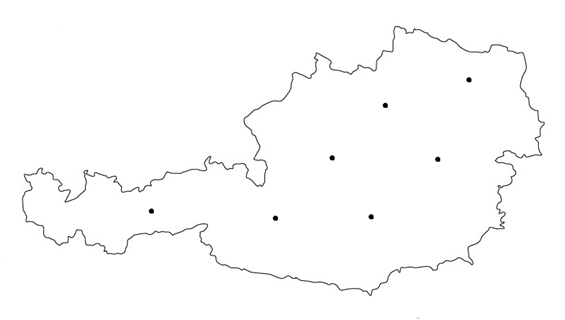
\includegraphics[height=6cm,width=10cm]{images/CSS_System}
	\caption{Beispiel eines CSS-Systems}
	\label{fig:CSS_System}
\end{figure}

\newpage
\subsection{Auswahl des Anbieters}
	Bei der Wahl des Anbieters, musste der Auftraggeber Best GmbH berücksichtigt werden. \\Folgende Punkte muss der Anbieter erfüllen:
	\begin{itemize}
		\item leichte Implementierung 
		\item es sollen alle gewünschten Funktionen umsetzbar sein 
		\item es soll möglichst ohne viel extra Aufwand möglich sein  
		\item es soll nicht kostspielig sein 
	\end{itemize}

Um die Anbieter auf die gewünschten Anforderungen zu überprüfen, wurde die Tabelle \ref{tab: Vor- und Nachteile der Anbieter} angefertigt. Daten für diese Tabelle wurden den Quellen ... entnommen.

\begin{table}[h]

	\begin{tabular}{|l|l|l|l|l|}
		\hline
		Anbieter &
		Kosten &
		API's vorhanden &
		Umsetzbarkeit(Zeit) &
		Vorteile und Nachteile \\ \hline
		Google Maps &
		gering &
		ja &
		ja &
		\begin{tabular}[c]{@{}l@{}}viele API's,\\ die die Arbeit erleichtern;\\ einfache Einbindung auf der Website;\\ performant;\\ großflächig aufgeschlossen;\\ Daten nur für den\\ Betreiber selbst einsehbar\end{tabular} \\ \hline
		Open Street Map &
		keine &
		nein &
		nein &
		\begin{tabular}[c]{@{}l@{}}keine API's vorhanden;\\ viel mehr Aufwand,\\ um das Gleiche wie\\ Google Maps zu bieten;\\ unperformant;\\ keine großflächige Aufschließung;\\ Daten sind für Jeden einsehbar\end{tabular} \\ \hline
		Geoinformationssystem &
		sehr hohe &
		nein &
		nein &
		\begin{tabular}[c]{@{}l@{}}genaue Ortung der Systeme;\\ sehr preisintensiv;\\ sehr zeitintensiv und komplex\end{tabular} \\ \hline
		CSS-System &
		keine &
		nein &
		ja &
		\begin{tabular}[c]{@{}l@{}}keine API's;\\ sehr viel Aufwand;\\ erfüllt den gleichen Zweck \\wie eine Karte\end{tabular} \\ \hline
	\end{tabular}
\caption{Vor- und Nachteile der Anbieter}
\label{tab: Vor- und Nachteile der Anbieter}
\end{table}


\newpage
Auf Basis der Tabelle \ref{tab: Vor- und Nachteile der Anbieter}, einigten sich der Auftraggeber und das Projektteam darauf, einen Kartendienst zu verwenden, da ein Geoinformationssystem zu anspruchsvoll gewesen wäre und ein CSS-System genau das Gleiche wie eine Karte wäre, nur mit mehr Aufwand verbunden ist. Daraufhin wurde vom Projektteam das Dokument “Google Maps vs Open Street Map” erstellt. Dieses Dokument ist auf der DVD der Diplomarbeit ersichtlich. Nach gemeinsamer Begutachtung dieses Dokuments und dem Abwägen der Vor- und Nachteile jedes Anbieters, haben sich der Auftraggeber und das Projektteam auf die Verwendung von Google Maps geeinigt. Google Map überwiegt klar in den Vorteilen gegenüber Open Street Map. Es ist zwar nicht kostenfrei, jedoch wird in der Regel bei normaler Benutzung der Website nie das Pensum von 300 Euro überschritten. 
\section{Berechtigungssystem Benutzer}
Im folgenden Abschnitt wird näher auf das Benutzerverwaltungssystem eingegangen sowie auf die vorhandenen Benutzerrollen, die einem Benutzer zugeteilt werden können.

\subsection{Benutzerrollen}
Die Weboberfläche bietet für deren Besucher ein rollenbasiertes Benutzersystem an, um die Funktionen für jeden Benutzer zu deklarieren.
Das rollenbasierte Benutzersystem unterscheidet zwischen folgenden Rollen:

\begin{itemize}
	\item Administrator 
	\item Mitarbeiter
	\item Öffentlicher Benutzer 
\end{itemize}



\subsubsection{Administrator}
Der Administrator-Benutzer ist der höchste Benutzer von allen. Er darf Energiesysteme sowie Energietechnologien erstellen und alle anderen vorhandenen bearbeiten und löschen. Zusätzlich dazu hat er Einsicht in sämtliche Grafana-Statistiken. Diese Benutzerrolle hat das Recht, neue Benutzer auf der Weboberfläche zu registrieren und vorhandene zu löschen, was für alle anderen Benutzer nicht möglich ist.

\subsubsection{Mitarbeiter}
Die Rolle „Mitarbeiter“ darf auf der Weboberfläche neue Energiesysteme sowie Energietechnologien erstellen. Die von ihm erstellten Energiesysteme sowie Energietechnologien kann er bearbeiten oder  löschen, und er hat auf diesen ebenso die Berechtigung auf Einsicht der Statistiken. Andere Mitarbeiter dürfen seine Energiesysteme und Energietechnologien nicht bearbeiten oder löschen und haben keinen Zugriff auf dessen Statistiken mit Ausnahme des Administrators. Ein Mitarbeiter-Benutzer darf somit nur seine selbst erstellten Energiesysteme und Energietechnologien verwalten. Der Mitarbeiter-Benutzer hat nicht die Berechtigung, neue Benutzer zu registrieren oder vorhandene zu löschen.

\subsubsection{öffentlicher Benutzer}
Dieser Benutzer hat die geringste Berechtigung und tritt in Kraft, wenn man nicht auf der Weboberfläche angemeldet ist. Dieser Benutzer darf keine Energiesysteme sowie Energietechnologien erstellen, bearbeiten oder löschen. Zusätzlich hat der öffentliche Benutzer keine Einsicht auf sämtliche Grafana-Statistiken. Der Zugang zu der Benutzerverwaltung ist ebenso nicht erreichbar. Dieser Benutzer sieht lediglich die öffentlichen Daten, die für jedes Energiesystem und jede Energietechnologie preisgegeben werden.

\subsection{Berechtigungen in Laravel}
Im folgenden Abschnitt wird erklärt, wie in Laravel die zuvor genannten Benutzerrollen unterschieden werden.
Dafür bietet Laravel Authentifizierungsrichtlinien. Dabei kann mit den Befehlen @auth und @guest überprüft werden, ob der aktuelle Benutzer authentifiziert oder ein Gast ist. Je nach Authentifizierung und Rolle hat der Benutzer unterschiedliche Rechte sowie Funktionen zur Verfügung.
Für genauere Informationen, wie eine Berechtigungsüberprüfung in Laravel umgesetzt werden kann, siehe Quelle x.y.



\section{Ui/Ux Design}
Im Wort Ui/Ux Design steht das Ui für User Interface und Ux für User Experience. Es handelt davon, wie eine Website von einem Nutzer aufgefasst und wahrgenommen wird. Es beschreibt die Wirkung, die das Design auf einen Nutzer hat. Genauer beschreibt die User Experience wie sich ein Nutzer auf der Website fühlt oder wie er auf ihr navigieren kann. 
Ziel ist es, dem Benutzer ein möglichst entspanntes Gefühl zu geben und ihm bei Allem zu helfen. Das User Interface beschäftigt sich vielmehr mit der Website an sich. Man macht sich hierbei Gedanken, ob der Benutzer das Design ansprechend finden könnte, oder ob überall die idealen Elemente oder Elementgrößen gewählt wurden. Eine weitere Frage, die man sich im User Interface überlegt, ist was wirkt auf den Benutzer positiv und was negativ. Einige Methoden das Ui/Ux Design umzusetzen sind: 

\begin{itemize}
	\item erstellen eines Wireframes 
	\item Umfragen an Usern durchführen
	\item Fragebögen auf der Seite selbst 
	\item erstellen einer Übersicht mit den Anforderungen der Benutzer
\end{itemize}
Nützliche Programme zum Erstellen der besagten Dokumente  sind folgende: 
\begin{itemize}
	\item Kissmetrics
	\item Figma
	\item SimilarWeb
\end{itemize}
Informationen über Ui und Ux Design wurden der Quelle xy entnommen.

\subsection{Wireframe}
Ein Wireframe hilft dem Design Team eine grobe Struktur der Website vorzudefinieren. Bei der Erstellung eines Wireframes wird der visuelle Design Part komplett vernachlässigt. Bei einem Wireframe wird sich auf den Aufbau und die Position der Elemente konzentriert. Es ist meist in schwarz und weiß gehalten, da Farben bei diesem Aufbauprozess nur behindern würden. 
\subsection{Persona}
Eine Persona dient dazu, die Bedürfnisse und Ziele der Zielgruppe zu erfassen. Mithilfe der Persona kann auf Wünsche und Bedürfnisse der Benutzer während der Entwicklung eingegangen werden. Empfohlen wird pro Zielgruppe um die fünf bis sechs Personen die das Produkt testen. Erstellt werden sie dann auf Grundlage von:
\begin{itemize}
	\item Interviews mit dem Benutzer
	\item Benutzertests
	\item Umfragen
\end{itemize}

\section{Template Layout}\label{sec: Layout}
Laravel bietet die Möglichkeit, mithilfe einer Layout Datei, Codeabschnitte auf mehreren Seiten zu verwenden. Hauptsächlich wird diese Funktion genutzt, um statische Elemente, die auf jeder Unterseite gleich sind, nur einmal zu programmieren. Ein gutes Beispiel wäre der Header oder auch der Footer, da diese Elemente auf den Unterseiten nicht variieren. 

\subsection{Platzhalter Yield}
In der Layout Datei kann @yield verwendet werden, um Platz zu halten. Dies ermöglicht es, beispielsweise den Titel der Website individuell für jede Unterseite zu setzen. Der Platzhalter wird in der Layout Datei folgendermaßen konfiguriert: 
\definecolor{mygray}{RGB}{252,251,244}
\renewcommand{\lstlistingname}{Quellcode}

\begin{lstlisting}[
	caption={Platzhalter in der Layout Datei Konfigurieren},
	label=Code,
	language=octave,
	numbers=left,
	firstnumber=1,
	numberfirstline=false,
	backgroundcolor=\color{mygray},
	basicstyle=\footnotesize=15,
	keywordstyle=\color{blue}
	]
	<title>@yield('title')</title>
\end{lstlisting} 
Möchte man diesen Platzhalter dann auf einer der Unterseiten, welche die Layout Datei verwenden, setzen, ist das folgendermaßen möglich:
\begin{lstlisting}[
	caption={Platzhalter auf einen Wert setzen},
	label=Code,
	language=octave,
	numbers=left,
	firstnumber=1,
	numberfirstline=false,
	backgroundcolor=\color{mygray},
	basicstyle=\footnotesize=15,
	keywordstyle=\color{blue}
	]
	@section('title', 'titlename')
\end{lstlisting} 
Das Projektteam verwendet dieses Statement auf jeder Unterseite, um den Titel zu setzen.

\subsection{Sections}
Sections ermöglichen es, die Layout Datei in Abschnitte zu unterteilen. Der Beginn einer Section wird mit folgendem Befehl gekennzeichnet:
\begin{lstlisting}[
	caption={Beginn einer Section kennzeichnen},
	label=Code,
	language=octave,
	numbers=left,
	firstnumber=1,
	numberfirstline=false,
	backgroundcolor=\color{mygray},
	basicstyle=\footnotesize=15,
	keywordstyle=\color{blue}
	]
	@section('sectionname)
\end{lstlisting} 
Um die Section wieder zu schließen, muss folgendes Statement benutzt werden: 
\begin{lstlisting}[
	caption={Ende einer Section kennzeichnen},
	label=Code,
	language=octave,
	numbers=left,
	firstnumber=1,
	numberfirstline=false,
	backgroundcolor=\color{mygray},
	basicstyle=\footnotesize=15,
	keywordstyle=\color{blue}
	]
	@endsection
\end{lstlisting} 
 Die Einteilung des Codes in Section erlaubt es, dieses Codestück auf einer anderen Seite mit nur einem Stichwort einzubinden. 
\subsection{Einbindung der definierten Sections}
Um diese im Layout File definierten Sections im Code einbinden zu können, müssen einige Einstellungen vorgenommen werden. Am Anfang einer neuen Seite muss dieser Code eingefügt werden:
\begin{lstlisting}[
	caption={Einbindung der Layout Datei},
	label=Code,
	language=octave,
	numbers=left,
	firstnumber=1,
	numberfirstline=false,
	backgroundcolor=\color{mygray},
	basicstyle=\footnotesize=15,
	keywordstyle=\color{blue}
	]
	@extends('layoutfilenname')
\end{lstlisting} 


Damit wird der Seite mitgeteilt, dass die angegebene Seite als Layout Vorlage verwenden werden soll. Wenn diese Zeile vorhanden ist, können mittels\@section('sectioname') die im Layout File definierten Sections eingebunden werden. Wichtig ist,  jedesmal nach dem @section auch ein @endsection einzugeben, sonst wird die Section nicht angezeigt. Zur Ergänzung der Section kann man den zu ergänzenden Code einfach zwischen dem @section und dem @endsection platzieren. Dieser wird dann zum bereits vordefinierten Code ergänzt.
\newpage
\section{Laravel Befehle}\label{sec Laravel Befehle}
Laravel bietet die Möglichkeit, viele Dinge mithilfe der Konsole Models, Controller oder Views, automatisch generieren zu lassen. In den folgenden Unterkapiteln werden die Wichtigsten dieser Befehle aufgelistet und kurz erklärt.
\subsection{Migration Befehle}\label{sec Migration Befehle}
Um eine neue Migration zu erstellen, muss folgendes Kommando in der Commandline ausgeführt werden:
\definecolor{mygray}{RGB}{252,251,244}
\renewcommand{\lstlistingname}{Quellcode}

\begin{lstlisting}[
	caption={Erstellen einer neuen Migration},
	label=Code,
	language=octave,
	numbers=left,
	firstnumber=1,
	numberfirstline=false,
	backgroundcolor=\color{mygray},
	basicstyle=\footnotesize=15,
	keywordstyle=\color{blue}
	]
php artisan make:migration migration_name
\end{lstlisting}
Wenn die Migration erfolgreich erstellt und initialisiert wurde, kann man mit folgendem Kommando die up() Methode aller Migrations aufrufen:
\definecolor{mygray}{RGB}{252,251,244}
\renewcommand{\lstlistingname}{Quellcode}

\begin{lstlisting}[
	caption={Aufruf der up() Methode in der Migration},
	label=Code,
	language=octave,
	numbers=left,
	firstnumber=1,
	numberfirstline=false,
	backgroundcolor=\color{mygray},
	basicstyle=\footnotesize=15,
	keywordstyle=\color{blue}
	]
	php artisan migrate
\end{lstlisting}
Nach Ausführung dieses Kommandos sind alle Tabellen in der Datenbank so wie gewünscht erstellt. 
Um alle ausgeführten Migrations anzeigen zu lassen, muss dieses Kommando verwendet werden:
\definecolor{mygray}{RGB}{252,251,244}
\renewcommand{\lstlistingname}{Quellcode}

\begin{lstlisting}[
	caption={Befehl um den Status der Migrations zu bekommen},
	label=Code,
	language=octave,
	numbers=left,
	firstnumber=1,
	numberfirstline=false,
	backgroundcolor=\color{mygray},
	basicstyle=\footnotesize=15,
	keywordstyle=\color{blue}
	]
php artisan migrate:status
\end{lstlisting}
Wenn die zuletzt erstellten Tabellen rückgängig gemacht werden sollen, gibt es die Möglichkeit, folgendes Kommando auszuführen:
\definecolor{mygray}{RGB}{252,251,244}
\renewcommand{\lstlistingname}{Quellcode}

\begin{lstlisting}[
	caption={Migrations rückgängig machen},
	label=Code,
	language=octave,
	numbers=left,
	firstnumber=1,
	numberfirstline=false,
	backgroundcolor=\color{mygray},
	basicstyle=\footnotesize=15,
	keywordstyle=\color{blue}
	]
	php artisan migrate:rollback 
\end{lstlisting}
Weitere nützliche Befehle sind unter  der Quelle xy () zu finden.

\subsection{Seeder und Factory Befehle}
Um einen Datenbank Seeder zu erstellen, ist folgendes Kommando notwendig: 
\begin{lstlisting}[
	caption={Datenbank Seeder erstellen},
	label=Code,
	language=octave,
	numbers=left,
	firstnumber=1,
	numberfirstline=false,
	backgroundcolor=\color{mygray},
	basicstyle=\footnotesize=15,
	keywordstyle=\color{blue}
	]
php artisan make:seeder seeder_name
\end{lstlisting}
Wenn eine Factory erstellt werden soll, gibt es folgende Möglichkeit:
\begin{lstlisting}[
	caption={Datenbank Factory erstellen},
	label=Code,
	language=octave,
	numbers=left,
	firstnumber=1,
	numberfirstline=false,
	backgroundcolor=\color{mygray},
	basicstyle=\footnotesize=15,
	keywordstyle=\color{blue}
	]
	php artisan make:factory factory_name
\end{lstlisting}
\newpage
Um den Seeder nach Initialisierung auszuführen, gibt es folgende Möglichkeit:
\begin{lstlisting}[
	caption={Datenbank Seeder ausführen},
	label=Code,
	language=octave,
	numbers=left,
	firstnumber=1,
	numberfirstline=false,
	backgroundcolor=\color{mygray},
	basicstyle=\footnotesize=15,
	keywordstyle=\color{blue}
	]
	php artisan db:seed
\end{lstlisting}
Weitere nützliche Befehle und Individualizations Möglichkeiten sind unter der Quelle xy() verzeichnet.
\subsection{Model und Controller Befehle}
Um ein neues Model zu erstellen, verwendet man dieses Kommando:
\begin{lstlisting}[
	caption={Erstellen eines neuen Models},
	label=Code,
	language=octave,
	numbers=left,
	firstnumber=1,
	numberfirstline=false,
	backgroundcolor=\color{mygray},
	basicstyle=\footnotesize=15,
	keywordstyle=\color{blue}
	]
php artisan make:model model_name
\end{lstlisting}
Um einen normalen Controller anzulegen, gibt es folgendes Kommando:
\begin{lstlisting}[
	caption={Erstellen einers neuen Controllers},
	label=Code,
	language=octave,
	numbers=left,
	firstnumber=1,
	numberfirstline=false,
	backgroundcolor=\color{mygray},
	basicstyle=\footnotesize=15,
	keywordstyle=\color{blue}
	]
	php artisan make:controller controller_name
\end{lstlisting}
Es gibt ergänzend die Möglichkeit, einen Resource Controller anzulegen. 
Ein Resource Controller hat den Vorteil, dass er vorgenerierte Methoden besitzt, wie zum Beispiel:
\begin{itemize}
	\item index()
	\item create()
	\item store()
	\item show()
	\item edit()
	\item update()
	\item destroy()
\end{itemize}
Erstellt wird ein Resource Controller folgendermaßen:
\begin{lstlisting}[
	caption={Erstellen einers neuen Resource Controllers},
	label=Code,
	language=octave,
	numbers=left,
	firstnumber=1,
	numberfirstline=false,
	backgroundcolor=\color{mygray},
	basicstyle=\footnotesize=15,
	keywordstyle=\color{blue}
	]
	php artisan make:controller controller_name --resource
\end{lstlisting}
Genauere Informationen zu der Erstellung von Models und Controllern finden Sie unter der Quelle xy ().

\subsection{Starten des Laravel Entwicklungs Servers}
Laravel bietet die Möglichkeit, wenn PHP auf dem Entwicklungssystem installiert ist, einen PHP Development Server zu hosten und das Projekt über den Localhost anzuzeigen. Um den Server zu starten, muss folgende Zeile eingeben werden:
\begin{lstlisting}[
	caption={Start des Laravel Entwicklungs Servers},
	label=Code,
	language=octave,
	numbers=left,
	firstnumber=1,
	numberfirstline=false,
	backgroundcolor=\color{mygray},
	basicstyle=\footnotesize=15,
	keywordstyle=\color{blue}
	]
	php artisan serve
\end{lstlisting}
Nach Ausführen dieses Kommandos kann man das Projekt unter http://localhost:8000 aufgerufen.


\subsection{Befehle nach dem Git Pull} \label{sec: Git}
Bei Team Projekten in Laravel ist Git die beste Lösung. Jedoch kommt es oft zu Komplikationen beim Herunterladen des Projekts durch Git. Es gibt aber einige Befehle, die es ermöglichen, das Laravel Projekt komplikationsfrei zu starten.
Dieser Kommand sorgt dafür, dass der APP\_KEY in der .env Datei richtig gesetzt wird:
\begin{lstlisting}[
	caption={APP\_Key generieren },
	label=Code,
	language=octave,
	numbers=left,
	firstnumber=1,
	numberfirstline=false,
	backgroundcolor=\color{mygray},
	basicstyle=\footnotesize=15,
	keywordstyle=\color{blue}
	]
php artisan key:generate 

\end{lstlisting}
Um sicher zu stellen, dass alle nötigen Pakete installiert wurden, kann folgender Befehl verwendet werden:
\begin{lstlisting}[
	caption={Alle nötigen Pakete installieren },
	label=Code,
	language=octave,
	numbers=left,
	firstnumber=1,
	numberfirstline=false,
	backgroundcolor=\color{mygray},
	basicstyle=\footnotesize=15,
	keywordstyle=\color{blue}
	]
	composer update
	
\end{lstlisting}
Nach Durchführung dieser Schritte sollte sich das Programm problemlos starten und verändern lassen.


\newpage
\section{Routen in Laravel}
Laravel verfügt über ein ausgedehntes Routing System über welches Views aber auch ganze Gruppen von Elementen angesprochen und angezeigt werden können. Diese Routen werden in der Datei “web.php” angelegt und verwaltet.
\subsection{Ressource Routen} 
Mit der Ressource Route wird ein ganzer Controller angesprochen, so können über diese Route alle Methoden in diesem Controller angesprochen und verwendet werden. Im Produkt wird jeder Controller, welcher wiederum für jede Tabelle vorhanden ist, durch eine Ressource Route adressiert. Dieser Vorgang wird in Abbildung \ref{fig:ResourceRoute} veranschaulicht.

\begin{figure}[h]
	\centering
	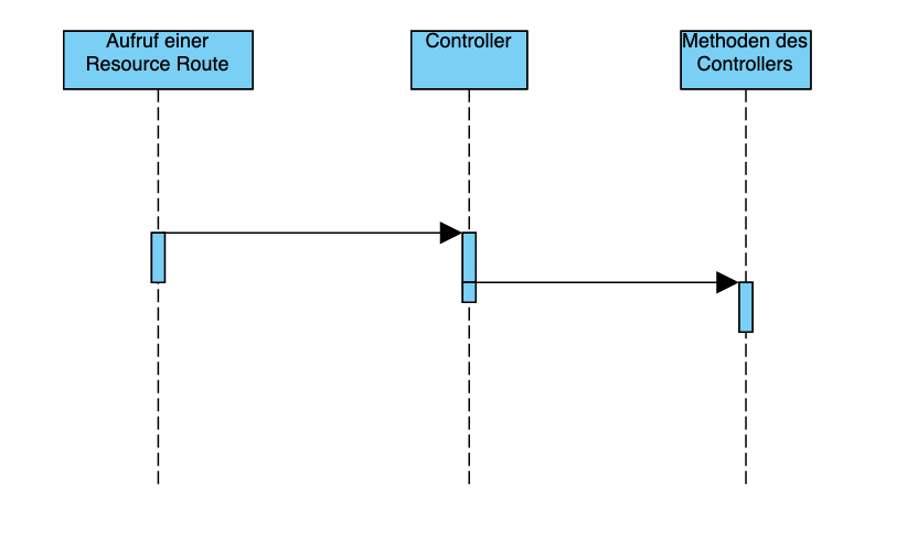
\includegraphics[height=6cm,width=9cm]{images/ResourceRoute}
	\caption{Aufbau einer Ressource Route}
	\label{fig:ResourceRoute}
\end{figure}

\subsection{GET Routen}
Mit diesem Typ von Routen lässt sich eine bestimmte Methode in einem ausgewählten Controller adressieren. Außerdem ist es möglich in einer GET Route einen Parameter mitzugeben welcher dann in der ausgewählten Methode im Controller verarbeitet wird. Im Produkt wird dieser Typ von Methoden verwendet, um beispielsweise die Startseite anzuzeigen. Weiters werden sie verwendet, um bestimmte Methoden in Controllern, zB. löschen von Energiesystemen, mit der Id des ausgewählten Objektes auszuführen. Am meisten kommt dieser Typ von Routen beim Erstellen, Editieren oder Löschen von Datenbankeinträgen zum Einsatz, da hier ein gewisser Eintrag mit dem mitgelieferten Parameter einer Route adressiert werden kann. Der Aufbau dieser Route wird in Abbildung \ref{fig:GETRoute} verdeutlicht.


\begin{figure}[h]
	\centering
	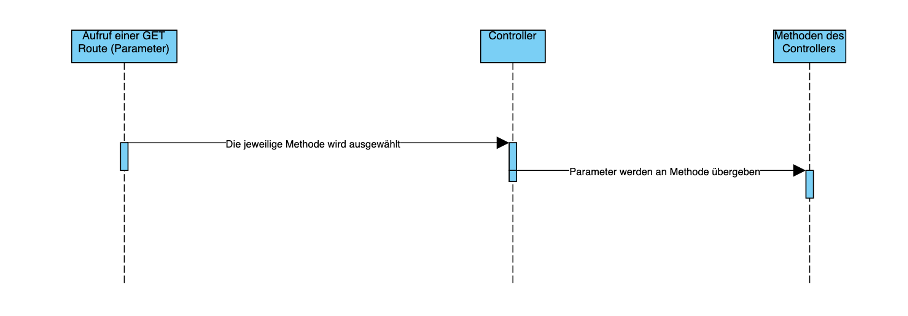
\includegraphics[height=6cm,width=16cm]{images/GETRoute}
	\caption{Aufbau einer GET Route}
	\label{fig:GETRoute}
\end{figure}
\newpage

\subsection{Auth Routen}
Sobald in Laravel das Authentifizierungssystem aktiviert wird, werden diese Routen automatisch erstellt. Diese Routen adressieren, die ebenfalls durch Laravel erstellen, auth Controller in der die Benutzeranmeldung sowie Registrierung bearbeitet wird.


\section{MVC}\label{sec: MVC}
Das Produkt verwendet das von Laravel bereitgestellte Design Pattern MVC (Model, View, Controller), welches in der Abbildung \ref{fig:MVC} dargestellt wird. 

\begin{figure}[h]
	\centering
	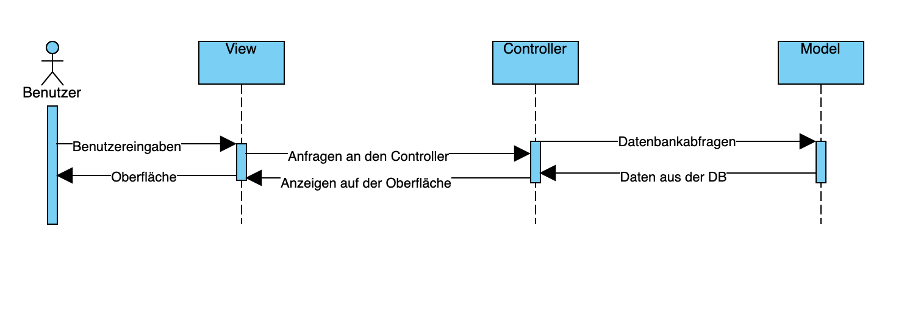
\includegraphics[height=6cm,width=18cm]{images/MVC}
	\caption{MVC Design Pattern}
	\label{fig:MVC}
\end{figure}

\subsection{Model}
Für jede durch eine Migration (Kapitel 3.2.2) erstellte Tabelle gibt es ein Model, in diesem wird wie der Name suggeriert, das Datenmodell abgebildet. Durch diesen Ansatz kann von jedem Model eine Instanz erstellt werden und so die Entsprechende Tabelle in einem beliebigen Programmabschnitt verwendet werden. Weiters werden in den Models die Relationen zwischen den einzelnen Tabellen beschrieben.
\subsection{View}
Das Produkt baut auf acht Views auf. In diesen Views werden die Daten, welche von den Controllern übergeben werden mithilfe von DataTables (Kapitel 3.6) dem Benutzer angezeigt. Weiters gibt es in den Views verschiedene Möglichkeiten der Benutzerinteraktion.
\subsection{Controller}
In den Controllern wird der Datenweg zwischen den Views, also den Benutzerinteraktionen und der Datenbank gesteuert. Für jede, durch eine Migration in der Datenbank erstelle Tabelle, gibt es einen Controller, welcher das Speichern, die Ausgabe, das Editieren sowie das Löschen von einzelnen Tupeln aus der Datenbank steuert. Weiters werden in den "store()" und "destroy()" Methoden des EnTechControllers sowie des EnSysControllers die API Aufrufe an die Grafana HTTP API mit den vom Benutzer eingegebenen Daten ausgeführt.

\chapter{Ergebnisdokumentation }
Dieser Abschnitt beinhaltet eine Dokumentation der verwendeten Werkzeuge zur Umsetzung der einzelnen Funktionen. Es werden alle behandelten Teilbereiche erläutert.

\section{Laravel }
In diesem Kapitel werden die Ergebnisse und Erfahrungen dokumentiert, welche sich im Laufe der Produktentwicklung mit dem Laravel Framework heraus kristallisiert haben.

\subsection{Installation}
Die Installation von Laravel erfolgt mithilfe des PHP Installations Tools Composer. Dieser installiert hierzu die Paketquellen Lokal auf dem System. Beim Erstellen eines neuen Laravel Projekts werden die von Composer installierten Quelldateien in das Verzeichnis des neu zu erstellenden Projekts kopiert und installiert. Im nachfolgenden Link ist mehr über die Installation von Laravel zu lesen:

Unter der Quelle xy () ist mehr über Laravel zu lesen.



\subsection{Bootstrap Einbindung}
Für das Design des Front-Ends wird die CSS Bibliothek “Bootstrap” (Kapitel 2.3.6.1) verwendet. Hierzu werden die Quelldateien von Bootstrap durch Composer lokal abgespeichert und durch den Laravel Befehl "php artisan ui bootstrap“ dem Laravel Projekt hinzugefügt. Laravel bietet die Möglichkeit beim Hinzufügen von Bootstrap mit der Option “-- auth” direkt die Beispielseiten (Login, Registrieren) für den Authentifizierungsvorgang zu erstellen. Im nachfolgenden Link ist mehr über die Installation von Bootstrap zu lesen:
\href{https://www.positronx.io/how-to-properly-install-and-use-bootstrap-in-laravel/}{Dokumentation der Installation}


\subsection{Grafana Einbindung}
Das Produkt kommuniziert mit dem Grafana Server über die von Grafana bereitgestellte HTTP API. Laravel verfügt hierzu über das Paket “guzzle-http”, welches es ermöglicht, mithilfe von wenigen Zeilen PHP Code einen HTTP Aufruf an eine bestimmte Quelle abzusenden.
\begin{figure}[h]
	\centering
	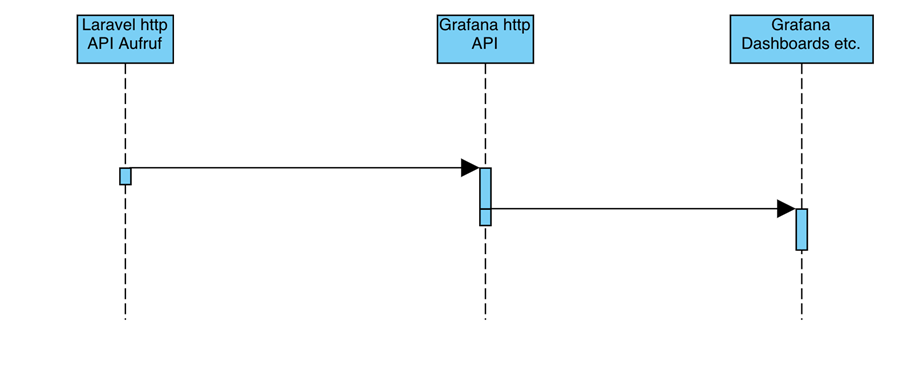
\includegraphics[height=6cm,width=18cm]{images/GrafanaEinbindung}
	\caption{Grafana Einbindung}
	\label{fig:GrafanaEinbindung}
\end{figure}




\newpage
\section{Datenbankanbindung in Laravel}
Um die Datenbank an das Programm anzubinden, müssen einige Änderungen in der .env Datei vorgenommen werden. Genauere Information zur .env Datei befinden sich im Kapitel  \ref{sec:Laravel .env Datei}. Welche Konfigurationen genau getätigt werden, können in den nachfolgenden Kapiteln nachgelesen werden. 

\subsection{Datenbank Anmeldeinformationen}
Eine Änderung war es, die Datenbank Anmeldeinformationen auf die richtigen Einstellungen zu setzen. Welche Attribute gesetzt werden, und was genau bei diesen Eingetragen werden muss, ist in Tabelle 3.1 ersichtlich. Eine mögliche Konfiguration ist in Tabelle 3.2 ersichtlich.
\begin{table}[h]
	\begin{tabular}{|l|l|}
		\hline
		Attribut         & Was soll eingetragen werden                        \\ \hline
		DB\_CONNECTION     & Hier muss die Zugriffsvariante auf die Datenbank  eingetragen werden                \\ \hline
		DB\_HOST          &  Hier muss die Domain des Datenbankservers, beispielsweise 127.0.0.1,\\& wenn der Datenbankserver über den Localhost bereitgestellt wird, eingeben werden    \\ \hline
		DB\_PORT       & Hier der Port über welchen zugegriffen werden soll \\ \hline
		DB\_DATABASE      & Hier der Name der Datenbank ,\\& auf welche zugegriffen werden soll\\
		DB\_USERNAME   & Der Benutzer, mit welchem zugegriffen werden soll              \\ \hline
		DB\_PASSWORD    & Das Passwort zum Benutzer\\ \hline
	\end{tabular}
\caption{Datenbank Anmeldeinformationen}
\label{sec: Datenbank Anmeldeinformationen}
\end{table}
\begin{table}[h]
	\begin{tabular}{|l|l|}
		\hline
		Attribut         & Was bei diesem Produkt eingetragen wurde                       \\ \hline
		DB\_CONNECTION     & mysql                 \\ \hline
		DB\_HOST          &  127.0.0.1\\ \hline
		DB\_PORT       & 3306\\ \hline
		DB\_DATABASE      & laravel\\
		DB\_USERNAME   & root             \\ \hline
		DB\_PASSWORD    & Hier wurde nicht eingetragen\\ \hline
	\end{tabular}
	\caption{Datenbank Anmeldeinformationen Beispiel}
	\label{sec: Datenbank Anmeldeinformationen Beispiel}
\end{table}
\newpage
\subsection{Mail Server Konfigurationen}
Um auf der Weboberfläche das Passwortzurücksetzen mittels E-Mail zu ermöglichen, muss Laravel eine E-Mail versenden. Dazu braucht es die nötigen Konfigurationen in der .env Datei. In der Tabelle 3.3 ist ersichtliche, welche Attribute gesetzt werden müssen, und welche Bedeutung diese haben.
\begin{table}[h]
	
	\begin{tabular}{|l|l|}
		\hline
		Attribut         & Was soll eingetragen werden                        \\ \hline
		MAIL\_MAILER     & Hier muss das Protokoll eingetragen                     \\ \hline
		Mail\_HOST          & Hier wird die Host Domain  eingegeben,\\&also welcher SMTP Server verwendet werden soll         \\ \hline
		MAIL\_PORT       & Der Port über welchen zugegriffen werden soll \\ \hline
		MAIL\_USERNAME      & Hier muss die E-Mail Adresse,\\& welche zum Absenden der Mail verwendet wird, eingetragen werden \\ \hline
		MAIL\_PASSWORD   & Das dazugehörige Passwort zur Email                \\ \hline
		MAIL\_ENCRYPTION    & Hier gibt man an, mit welchem Verfahren verschlüsselt werden soll                             \\ \hline
		MAIL\_FROM\_ADDRESS & Die Adresse, welche beim Empfänger als Sender E-Mail angezeigt wird  eintragen                 \\ \hline
		MAIL\_FROM\_NAME & Der Name, der dem Empfänger angezeigt wird    \\ \hline
	\end{tabular}
\caption{Mail Server Konfigurationen}
\label{sec: Mail Server Konfigurationen}
\end{table}

Bei diesem Produkt hat die Konfiguration folgendermaßen ausgesehen:
\begin{table}[h]
	
	\begin{tabular}{|l|l|}
		\hline
		Attribut         & Was bei diesem Produkt eingetragen wurde                      \\ \hline
		MAIL\_MAILER     & smtp                     \\ \hline
		Mail\_HOST          & smtp.gmail.com         \\ \hline
		MAIL\_PORT       & 465 \\ \hline
		MAIL\_USERNAME      & marcelentner2@gmail.com  \\ \hline
		MAIL\_PASSWORD   & Das dazugehörige Passwort zur Email                \\ \hline
		MAIL\_ENCRYPTION    & ssl                             \\ \hline
		MAIL\_FROM\_ADDRESS & marcelentner2@gmail.com                       \\ \hline
		MAIL\_FROM\_NAME & Best GmbH  \\ \hline
	\end{tabular}
	\caption{Mail Server Konfigurationen Beispiel}
	\label{sec: Mail Server Konfigurationen Beispiel}
\end{table}
\newpage

\subsection{Migrations}
Die Migrations wurden dazu verwendet, um Tabellen zu gestalten. In ihnen wurden alle nötigen Attributnamen und deren Datentypen konfiguriert. Das Produkt verwendet folgende von Laravel automatisch erzeugten Migrations für die Benutzerauthentifizierung: 
\begin{itemize}
\item 2014\_10\_12\_000000\_create\_users\_table.php
\item 2014\_10\_12\_100000\_create\_password\_resets\_table.php
\item 2019\_08\_19\_000000\_create\_failed\_jobs\_table.php
\item 2019\_12\_14\_000001\_create\_personal\_access\_tokens\_table.php
\end{itemize}
Zusätzlich zu diesen bereits erstellten Migrations wurde für jede Energietechnologieart eine eigene Migration angelegt. Darüber hinaus wurden Templates\footnote{ein Template ist ein Grundbauplan} für ein Energiesystem und eine Energietechnologie erstellt. Im Energietechnologien Template sind alle Attribute, die bei jeder Energietechnologie gleich sind. Alle individuellen Attribute werden dann mithilfe der eigenen Migrations abgebildet.

\section{Datenbankdesign}
In diesem Kapitel der Diplomarbeit wird das Redesign der Datenbank und der Relationen zwischen den einzelnen Tabellen behandelt.


\subsection{Erstellen eines neuen Schemas}
Für das Produkt wurde ein neues vom alten unabhängiges Datenbankschema entwickelt. Hauptgründe hierfür waren die im Kapitel 2.1 festgestellten Mängel und Designfehler. Im neuen Design wurde darauf geachtet alle Design Richtlinien welche für Relationale Datenbanken gelten einzuhalten. Das neue Datenbankschema besteht aus 21 Tabellen für Individuelle Energietechnologien sowie aus einer Tabelle für Benutzer, einer Tabelle für erstellte Energiesysteme und einer Tabelle für die Generalisierung einiger Attribute von Energietechnologien.

\subsubsection{ER-Model}
Um das Datenbankdesign zu veranschaulichen und Unklarheiten mit dem Auftraggeber vorzubeugen, wurden mithilfe des Programms “MySql Workbench” ein EER (Extended Entity Relationship) Diagramm erstellt. In diesem Diagramm ist jede Tabelle mit ihren Attributen sowie Primär und Fremdschlüsseln abgebildet. Weiters sind auch die einzelnen Relationen zwischen einer oder Mehreren Tabellen veranschaulicht. Das vollständige EER Modell der Datenbank ist in der Abbildung 3.2 zu sehen.

\begin{figure}[h]
	\centering
	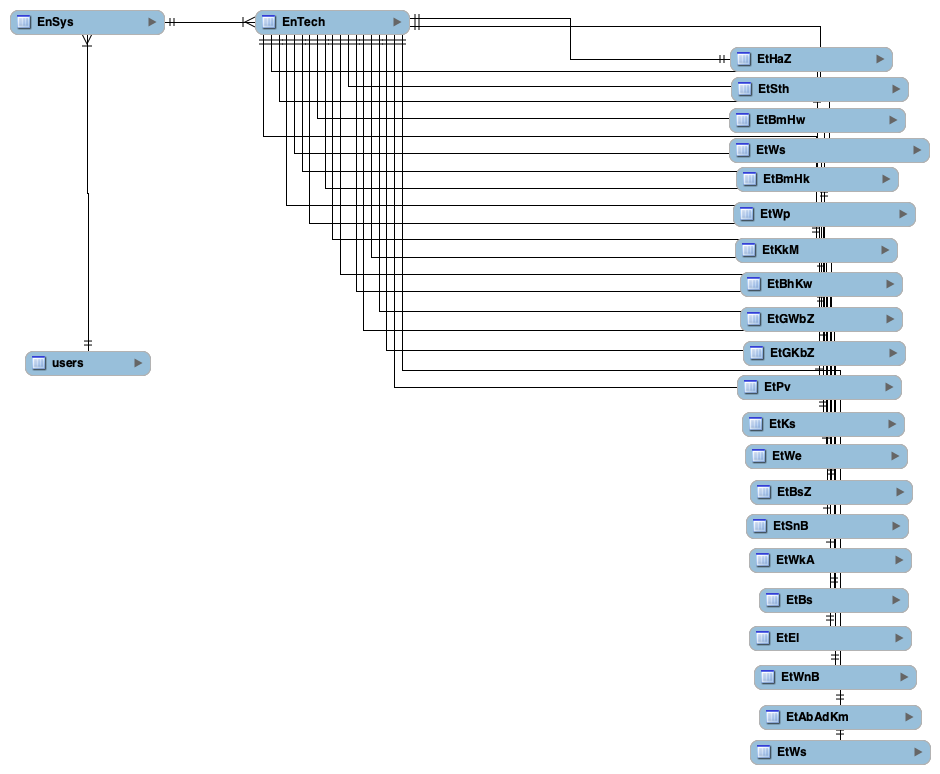
\includegraphics[height=15cm,width=18cm]{images/eer}
	\caption{ER Model}
	\label{fig:ERModel}
\end{figure}
\newpage
\subsubsection{Fremdschlüssel}
Wie im Kapitel 3.4.1.1 wurden zwischen den Tabellen verschiedene Relationen verwendet. Zwischen den Tabellen “users” und “EnSys” besteht eine 1:N Relation. Dies bedeutet, dass in jedem Eintrag in der “EnSys” Tabelle der Primärschlüssel des Benutzers welcher, den Eintrag durchführt, als Fremdschlüssel gespeichert wird. Zwischen den Tabellen “EnSys” und “EnTech” besteht ebenfalls eine 1:N Relation. In diesem Fall werden die Primärschlüssel der “users” sowie der “EnSys” Tabelle als Fremdschlüssel in der “EnTech” Tabelle gespeichert. Zwischen der “EnTech” sowie jeder der 21 Tabellen für individuelle Energietechnologien besteht eine 1:1 beziehung. Es gibt also zu jedem Eintrag in der “EnTech” Tabelle genau einen Eintrag in einer der 21 Tabellen für Energietechnologien. Hierbei wird der Primärschlüssel des Eintrages der “EnTech” Tabelle als Fremdschlüssel im korrespondierenden Eintrag in einer der 21 Tabellen für Energietechnologien gespeichert.



\section{Corporate Design}
Vom Projektteam wurde ein Corporate Design Manual erstellt. Dieses befindet sich auf der DVD der Diplomarbeit. In diesem Corporate Design Manual wurden folgende Themen bearbeitet: 
\begin{itemize}
	\item Oberfläche
	\item Definierte Farben
	\item Verwendung der definierten Farben
	\item Überschriften
	\item Buttons 
	\item Interaktionsfarben
	\item Schriftarten
	\item Schriftgrade
	\item Logo
	\item Verwendete Icons
	\item Bedeutung der Icons 
	\item Icons mit Funktionalitäten 	
	\item Website Design

\end{itemize}
Auf die wichtigsten Elemente wird in den nachfolgenden Kapiteln eingegangen.
\subsection{Vorschläge}
Nach Absprache der Grundanforderung des Produkts wurden, mithilfe der Adobe xd Software,  drei Designvorschläge verfasst. Diese sind ebenso auf der DVD der Diplomarbeit einsehbar. Um diese aussagekräftig zu vergleichen, wird von jedem Vorschlag, die Energiesystemseite visuell dargestellt. Dies ist in den drei nachfolgenden Abbildungen \ref{fig:Design Vorschlag 1},\space\ref{fig:Design Vorschlag 2},\space\ref{fig:Design Vorschlag 3} ersichtlich.
\begin{figure}[h]
	\centering
	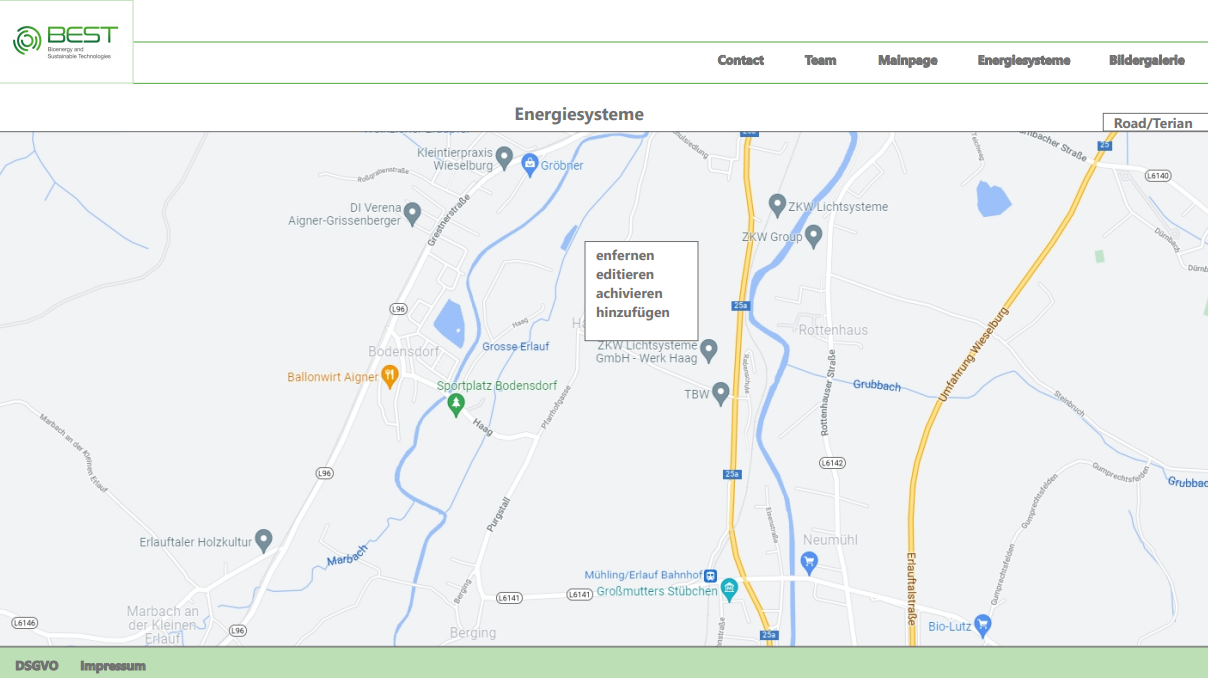
\includegraphics[height=6cm,width=12cm]{images/DesignVorschlag1}
	\caption{Design Vorschlag 1}
	\label{fig:Design Vorschlag 1}
\end{figure}
\newpage
\begin{figure}[h]
	\centering
	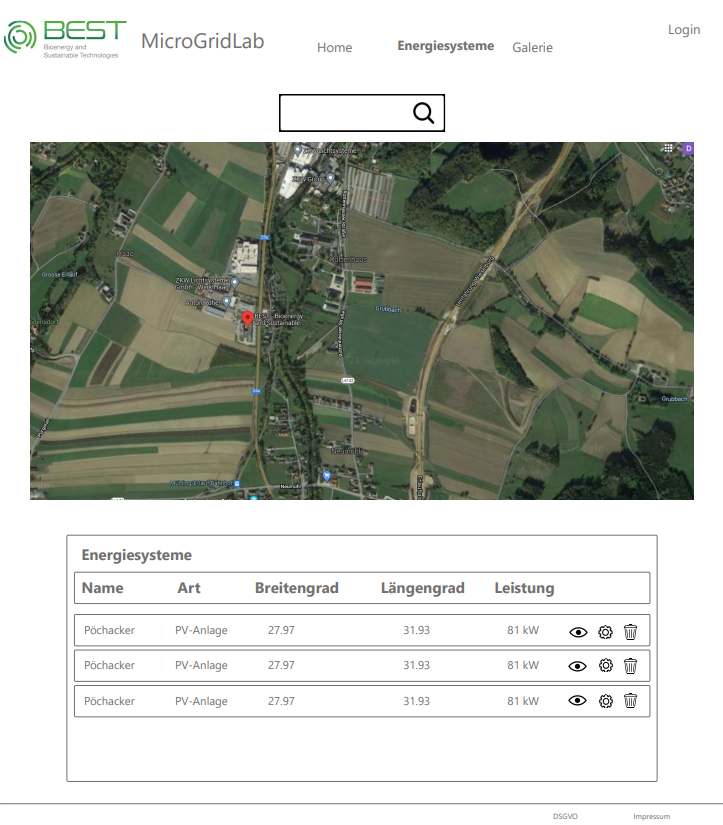
\includegraphics[height=12cm,width=11cm]{images/DesignVorschlag2}
	\caption{Design Vorschlag 2}
	\label{fig:Design Vorschlag 2}
\end{figure}
\begin{figure}[h]
	\centering
	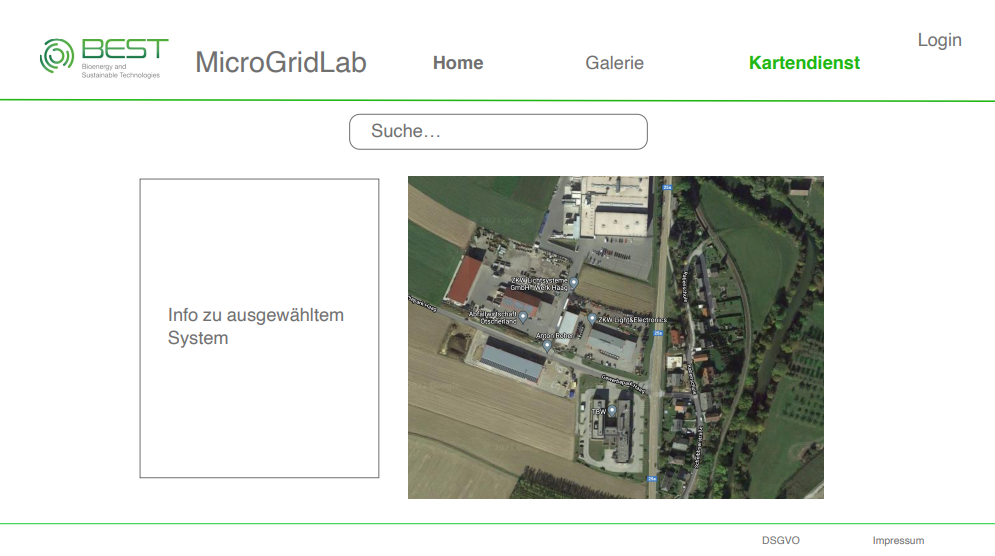
\includegraphics[height=7cm,width=12cm]{images/DesignVorschlag3}
	\caption{Design Vorschlag 3}
	\label{fig:Design Vorschlag 3}
\end{figure}
\subsection{Änderungsvorschläge} \label{sec:Änderungsvorschläge}
Die oben ersichtlichen Design Vorschläge wurden dem Auftraggeber über Skype präsentiert. Dieser favorisierte die Vorschläge \ref{fig:Design Vorschlag 1} und  \ref{fig:Design Vorschlag 2}. 
Von Seiten des Auftraggebers kamen viele Verbesserungsvorschläge und Ideen. Einige davon sind:
\begin{itemize}
	\item Die Liste soll neben der Map platziert werden.
	\item Es soll folgende Unterseiten geben:
	\subitem Home
	\subitem Energiesysteme
	\subitem Galerie
	\item Es soll Icons geben, welche es ermöglichen, Energiesysteme und Energietechnologien in der Liste zu löschen, bearbeiten oder einzusehen. 
	\item Es sollen die Farben aus der CSS Datei der bereits vorhanden Website extrahiert werden.
	
\end{itemize}


\subsection{Finales Design}
Nach genauer Definition der Änderungsvorschläge im Kapitel \ref{sec:Änderungsvorschläge}, wurde erneut in Adobe XD ein Design Vorschlag erstellt. Dieser Vorschlag war eine Mischung aus dem Vorschlag 1 und dem Vorschlag 2 mit den gewünschten Änderungen des Auftraggebers. Auch dieser Vorschlag ist auf der DVD der Diplomarbeit einsehbar. Um einen Vergleich zwischen Vorschlag 1 , Vorschlag 2 und dem finalen Design zu ermöglichen, wird nachfolgend auch die Energiesystem Seite des finalen Vorschlags visuelle dargestellt.

\begin{figure}[h]
	\centering
	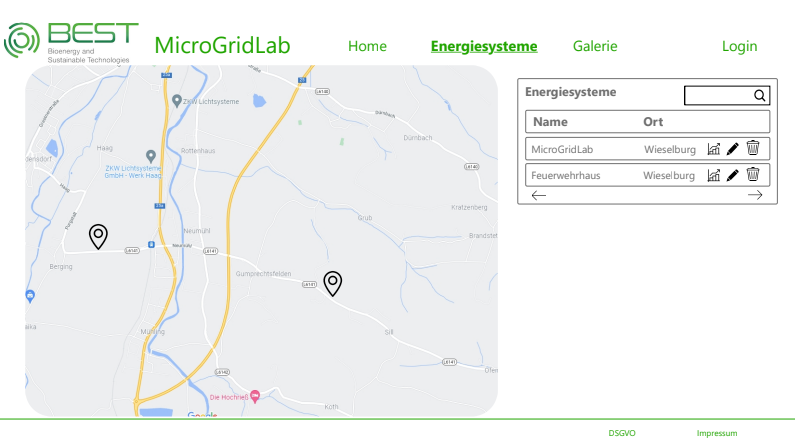
\includegraphics[height=7cm,width=12cm]{images/FinalerVorschlag}
	\caption{Finaler Design Vorschlag}
	\label{fig:Finaler Design Vorschlag}
\end{figure}
\newpage
Am Vorschlag in \ref{fig:Finaler Design Vorschlag}, wurde sich während der Entwicklung gerichtet. Aufgrund laufender Änderungswünsche des Auftraggebers variiert das finale Produktdesign jedoch stark vom finalen Vorschlag. Das finale Design ist im Kapitel \ref{sec: Front-End} einsehbar. 

\subsection{Definierte Farben}
Das Produktdesign basiert auf dem Front-End Framework Bootstrap. In Bootstrap werden alle Farben in der Datei “app.css” definiert. Hier ein textueller Ausschnitt, der vom Projektteam verwendeten Farben:
\\
\begin{itemize}
	\item --bs-primary: \#1b8836;
	\item --bs-blue: \#0d6efd;
	\item --bs-white: \#fff;
	\item --bs-danger: \#dc3545;
\end{itemize}
\newpage
Auf Wunsch des Auftraggebers wurden jedoch einige Farben aus den CSS Dateien der bereits vorhanden Website extrahiert und bei diesem Produkt verwendet. Folgende Farben wurden extrahiert:
\\
\\
\begin{tabular}{|c|c|c|c|c|}
	\hline
	Hex & CMYK & RGB & HSV & HSL \\
	\hline
	\#1b8836 & 80\%, 0\%, 60\%, 47\% & 27, 136, 54 & 135, 80\%, 53\% & 135, 67\%, 32\%  \\
	\hline 
	\#f8f9fa & 1\%, 0\%, 0\%, 2\% & 247, 250, 250 & 80, 1\%, 98\% & 80, 23\%, 97\% \\
	\hline
	\#e84d3d & 0\%, 67\%, 74\%, 9\% & 232, 77, 61 & 6, 74\%, 91\% & 6, 79\%, 57\% \\
	\hline
	\#212529 & 20\%, 10\%, 0\%, 84\% & 33, 37, 41 & 210, 20\%, 16\% & 210, 11\%, 15\% \\
	\hline
	\#f1f1f1 & 19\%, 10\%, 0\%, 84\% & 241, 241, 241 & 210, 20\%, 16\% & 210, 11\%, 15\% \\
	\hline
	\#0d6efd & 95\%, 57\%, 0\%, 1\% & 13, 109, 252 & 216, 95\%, 99\% & 216, 98\%, 52\% \\
	\hline
	\#21a500 & 80\%, 0\%, 100\%, 35\% & 33, 166, 0 & 108, 100\%, 65\% & 108, 100\%, 33\% \\
	\hline
	

\end{tabular}
	\\
\\
Alle verwendeten Farben sind im Corporate Design Manuel, auf der DVD der Diplomarbeit unter dem Kapitel  definierte Farben ersichtlich.

\subsection{Überschriften}
Überschriften werden bei diesem Produkt vorrangig verwendet, um anzuzeigen, über welches Thema der Fließtext, der sich meist direkt unter einer Überschrift befindet, handelt. Bei diesem Produkt wurden Überschriften der Gattung <h1>, <h2> und <h3> verwendet. Aus designtechnischen Gründen, befindet sich jede Überschrift immer direkt in der Mitte der Website. Jede Überschrift, welche außerhalb eines Fließtextes steht, ist in der Farbe \#1b8836 eingefärbt und in der Schriftart Smooch Snans formatiert. Überschriften, welche sich in einem Fließtext befinden, werden in der Farbe \#212529 eingefärbt. Folgende Überschriften sind beim Produkt vorhanden: 
\begin{itemize}
	\item Intelligente Strom- und Mikronetze
	\item Entwicklungsfelder und Anwendungsgebiete
	\item Forschungsprojekt Microgrid Lab
	\item Datenschutzerklärung
	\item DSGVO
	\item Impressum
\end{itemize}
\newpage
\begin{figure}[h]
	\centering
	\includegraphics[height=8cm,width=14cm]{images/UberschrieftenImFließtext}
	\caption{Überschriften im Fließtext}
	\label{fig: Überschriften im Fließtext}
\end{figure}
\begin{figure}[h]
	\centering
	
\includegraphics[height=8cm,width=14cm]{images/ImpressumUberschrift}
	\caption{Überschriften außerhalb des Fließtextes}
	\label{fig: Überschriften außerhalb des Fließtextes}
\end{figure}
\newpage

\subsection{Interaktionsfarben}
Interaktionsfarben werden verwendet, um eine Aktion zu kennzeichnen. Bei diesem  Produkt gibt es zwei verschiedene Interaktionsfarben. Die erste Farbe ist „\#21a500“ und die zweite „\#f1f1f1“. Die erste Farbe ist ersichtlich, wenn mit dem Mauszeiger über den DataTable\footnote{genauer in \autoref{sec:DataTable} erklärt} gefahren wird. Und die zweite Farbe wird ersichtlich, wenn mit dem Mauszeiger auf das Drop-Down in der Galerie gefahren wird, um ein Energiesystem auszuwählen. Wenn dies geschieht, verfärben sich die einzelnen Auswahlelemente in die Farbe „\#f1f1f1“. 
\begin{figure}[h]
	\centering
	\includegraphics[height=8cm,width=15cm]{images/InteraktionDatatable}
	\caption{Interaktion mit dem DataTable}
	\label{fig: Interaktion mit dem Datatabel}
\end{figure}
\begin{figure}[h]
	\centering
	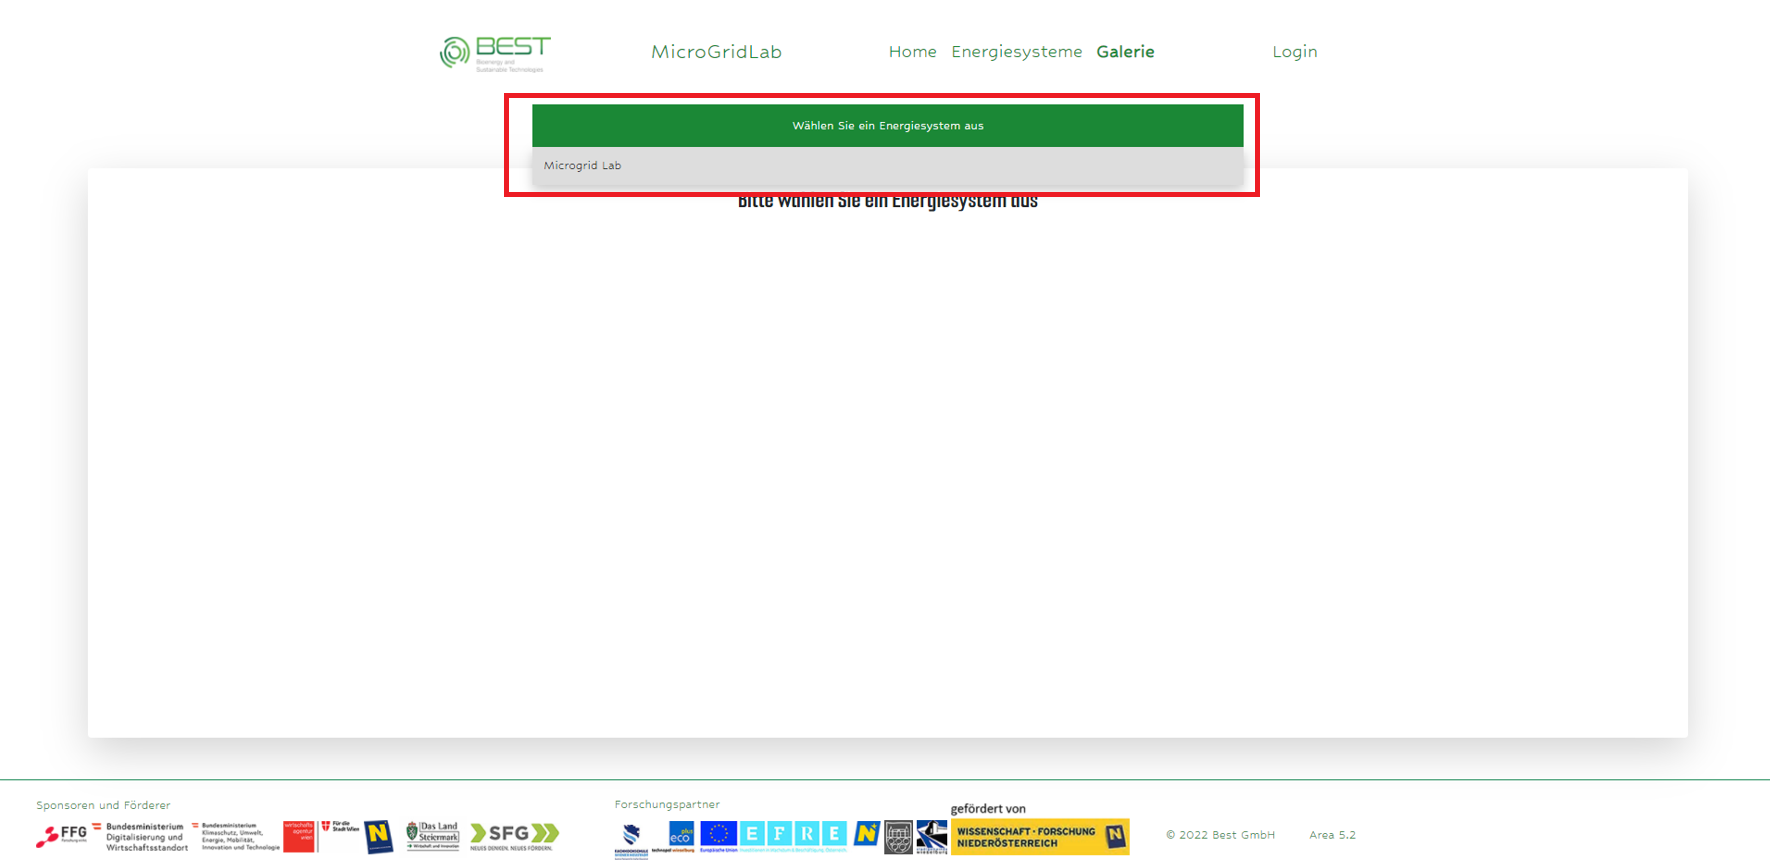
\includegraphics[height=8cm,width=15cm]{images/InteraktionDropDown}
	\caption{Interaktion mit dem Drop-Down in der Galerie}
	\label{fig: Interaktion mit dem Datatabel}
\end{figure}
\newpage

\subsection{Schriftarten}
Unser Produkt verwendet die Schriftarten Smooch Sans und Hubballi. Diese Schriftarten sind von Google Fonts frei zur Verfügung und zur Verwendung gestellt. Hubballi wurde für jede Art von Fließtext verwendet. Smooch Snans wurde verwendet, um die Überschriften zu formatieren. In der Abbildung \ref{fig: Beispiel auf der Website} sind beide Schriften veranschaulicht.
\begin{figure}[h]
	\centering
	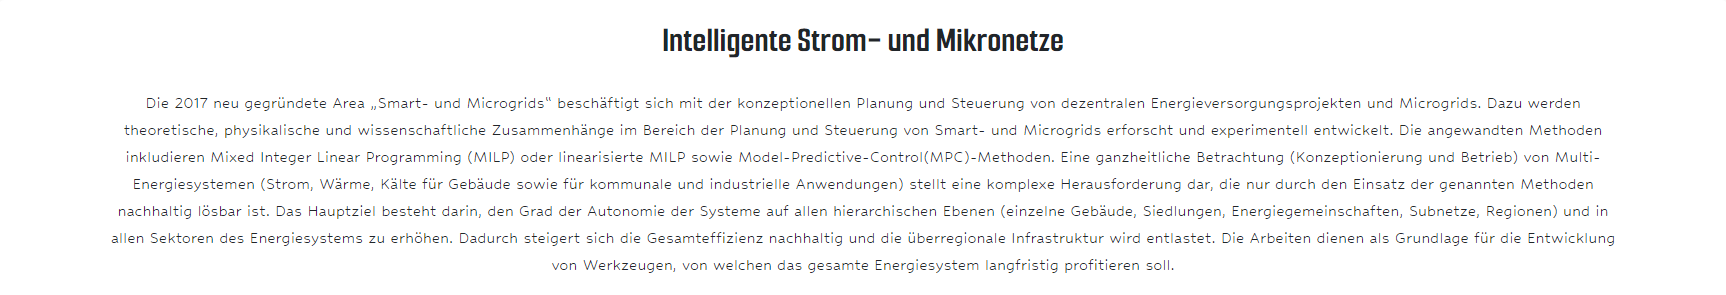
\includegraphics[height=5cm,width=15cm]{images/Beispiel_Schriftarten}
	\caption{Beispiel auf der Website}
	\label{fig: Beispiel auf der Website}
\end{figure}
\newpage
\subsection{Schriftgrade}
Die Schriftgrade variieren bei diesem Produkt nur bei der Anzeige der aktuellen Seite.
Die Überschriften Home, Energiesysteme und Galerie werden mithilfe des <b> Tags beim Besuchen der gleichnamigen Seite fett gemacht. Dadurch, dass die aktuelle Seite immer fett geschrieben wird, wird die Navigation durch das Produkt erleichtert.
\begin{figure}[h]
	\centering
	
\includegraphics[height=3cm,width=20cm]{images/Header}
	\caption{Header auf der Website}
	\label{fig: Header}
\end{figure}

\subsection{Logo}\label{sec: Logo}
Beim Logo hat sich das Projektteam an den Wunsch des Auftraggebers gehalten und ein Logo, welches von Seitens des Auftraggebers zur Verfügung gestellt wurde, verwendet. Zwei Logos wurden zur Verfügung gestellt und gemeinsam wurde sich auf das Logo in Abbildung \ref{fig: Logo1} geeinigt. Das Projektteam rät jedoch dazu, bei Logos SVG Grafiken zu verwenden und nicht wie in diesem Fall eine JPG Grafik. Da dies jedoch für den Auftraggeber keine Relevanz hatte, wurde wie besprochen das Logo aus Abbildung \ref{fig: Logo1}  verwendet.
\\
\begin{figure}[h]
	\centering
	\includegraphics[height=3cm,width=14cm]{images/Logo1}
	\caption{Logo 1}
	\label{fig: Logo1}
\end{figure}
\\
\begin{figure}[h]
	\centering
	\includegraphics[height=3cm,width=14cm]{images/Logo2}
	\caption{Logo2}
	\label{fig: Logo2}
\end{figure}

\newpage
\subsection{Verwendete Icons und deren Bedeutungen} \label{sec:Verwendete Icons und deren Bedeutungen}
Bei diesem Produkt werden Icons verwendet, um Energiesysteme oder Energietechnologien auf der Map visuell darzustellen. Ein weiteres Einsatzgebiet der Icons sind Formulare oder Übersichten. Auf diese Einsatzgebiete wird in den Kapiteln  \ref{sec: Map Icons} und \ref{sec: Icons in Formularen} genauer eingegangen. Wichtig zu unterscheiden sind Icons in schwarz-weiß und Icons in Farbe. Icons in Farbe werden verwendet um Energietechnologien oder Energiesysteme auf der Map dazustellen. Icons in schwarz-weiß werden verwendet um Daten anzuzeigen oder Funktionalitäten bereit zustellen.
Eine Liste mit allen Icons und deren Bedeutungen ist im Coperate Design Manuel auf der DVD der Diplomarbeit ersichtlich.




\subsection{Map Icons}\label{sec: Map Icons}
Das Produkt verwendet die vom Auftraggeber bereitgestellte Icons, um Energietechnologien oder Energiesystem auf der Karte visuelle darzustellen. Die Icons auf der Map sehen folgendermaßen aus:
\begin{figure}[h]
	\centering
	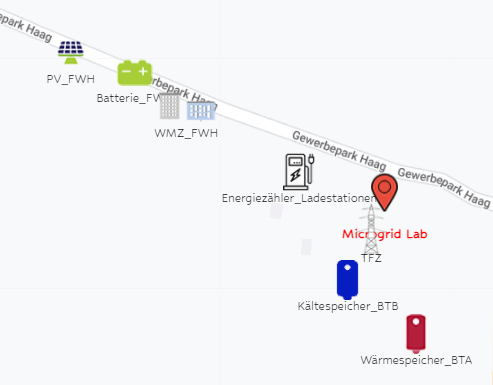
\includegraphics[height=6cm,width=10cm]{images/MapIcons}
	\caption{Icons auf der Map}
	\label{fig: Icons auf der Map}
\end{figure}
\\
Um Energiesysteme oder Energietechnologien zu verzeichnen, werden folgende Icons verwendet: 
\begin{figure}[h]
	\centering
	
\includegraphics[height=1cm,width=1cm]{images/Icons/esrot}
	\caption{Icon markiert ein Energiesystem}
	\label{fig: EnergiesystemIcon}
\end{figure}
\begin{figure}[h]
	\centering
	
\includegraphics[height=1cm,width=1cm]{images/Icons/etrot}
	\caption{Icon markiert eine Energietechnologie}
	\label{fig: EnergietechnologieIcon}
\end{figure}

\newpage

\subsection{Icons in Formularen}\label{sec: Icons in Formularen}
Alle weiteren verwendeten Icons wurden von flaticons.com implementiert. Diese Icons werden dazu genutzt, um in Formularen anzuzeigen, welche Art von Wert verlangt wird. Des Weiteren werden diese Icons in Übersichten verwendet, um dem Benutzer anzuzeigen, um welchen Wert es sich handelt. Um diese Icons jedoch verwenden zu dürfen, mussten alle Autoren in der Datenschutzseite verlinkt werden. Hier ein Beispiel, wie diese Anwendungsfälle auf der Website aussehen:
\begin{figure}[h]
	\centering
	\includegraphics[height=10cm,width=5cm]{images/IconsInÜbersichten}
	\caption{Icon in Übersichten}
	\label{fig: Icons in Übersichten}
\end{figure}
\newpage
\begin{figure}[h]
	\centering
	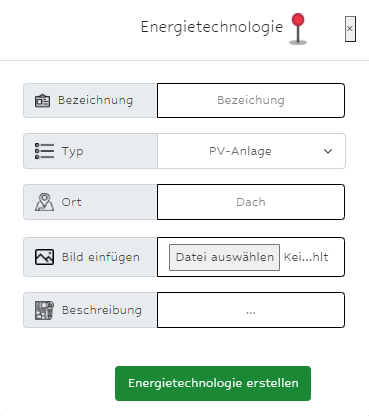
\includegraphics[height=6cm,width=5cm]{images/IconsInFormularen}
	\caption{Icon in Formularen}
	\label{fig: Icons in Formularen}
\end{figure}
Aus lizenztechnischen Gründen wurde jeder Autor eines Icons auf unserer Seite im Datenschutz verlinkt. Eine Verlinkung sieht folgendermaßen aus:
\begin{figure}[h]
	\centering
	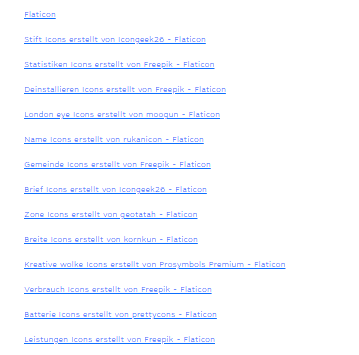
\includegraphics[height=1cm,width=8cm]{images/IconAutorVerlinkungen}
	\caption{Autoren Verlinkungen}
	\label{fig: Autoren Verlinkungen}
\end{figure}


\subsection{Icons im DataTable}
Folgende Icons werden  verwendet, um Energiesystem oder Energietechnologien zu bearbeiten, zu löschen oder auf deren Grafana Statistiken zuzugreifen.
\begin{table}[h]
	\begin{tabular}[t]{|l|l|}
		\hline
		Icon & Funktion                                                                                     \\ \hline
			
\includegraphics[height=1cm,width=1cm]{images/Icons/statistik}& Mit einem Klick auf dieses Icon öffnet sich ein Pop-up,\\& auf welchem die dazugehörigen  Grafana Statistiken präsentiert werden       \\ \hline
			
\includegraphics[height=1cm,width=1cm]{images/Icons/delete}  & Mit einem Klick auf dieses Icon wird das ausgewählte Energiesystem gelöscht                  \\ \hline
			
\includegraphics[height=1cm,width=1.5cm]{images/Icons/auge} & Mit einem Klick auf dieses Icon werden erweiterte Infos zu dem ausgewählten System angezeigt \\ \hline
			
\includegraphics[height=1cm,width=1cm]{images/Icons/stift} & Mit einem Klick auf dieses Icon öffnet sich eine Bearbeitungsmöglichkeit,\\& auf welcher man die Eigenschaften des Systems ändern kann \\ \hline
	\end{tabular}
	\caption{Icons im DataTabale}
\label{tab: Icons im DataTabales}
\end{table}
\newpage

Auf der Website werden diese Icons im DataTable hinter einer Energietechnologie oder einem Energiesystem eingeblendet. Dies sieht folgendermaßen aus:
\begin{figure}[h]
	\centering
	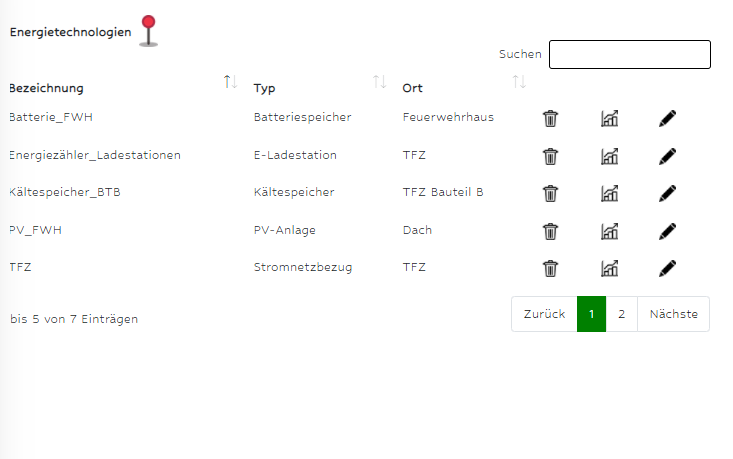
\includegraphics[height=10cm,width=15cm]{images/IconsImDatatable}
	\caption{Icons im DataTable}
	\label{fig: Icons im Datatable}
\end{figure}


\subsection{Buttons}
Buttons werden bei diesem Produkt ausschließlich genutzt, um Formulare abzusenden. Buttons befinden sich immer mittig unter einem Formular und  haben die Hintergrundfarbe \#1b8836. In Abbildung \ref{fig: Beispiel eines Buttons} \space ist ein Beispielbutton erschlich. 
\begin{figure}[h]
	\centering
	
\includegraphics[height=2cm,width=6cm]{images/BeispielButton}
	\caption{Beispiel eines Buttons}
	\label{fig: Beispiel eines Buttons}
\end{figure}
\newpage
\subsection{Tabelle mit generellen Informationen über einzelne HTML Elemente}
Hier ist wichtig zu definieren, für was welches HTML Element verwendet wurde. <h1>,  <h2> und <h3> wurden verwendet, um Überschriften zu definieren. In einem <p> Element befindet sich immer ein Fließtext. Mit dem <a> Element werden Links definiert. Bei diesem Produkt wurden im Header die Navigationsmöglichkeiten mit diesem Element versehen. 
\begin{table}[h]

	\begin{tabular}{|l|l|l|l|l|}
		\hline
		HTML Element                & Schriftart  & Größe  & Farbe              & Style class oder id   \\ \hline
		\textless{}h1\textgreater{} & Smooch Sans & 2em & \#1b8836  \#212529 & \begin{tabular}[c]{@{}l@{}}DsgvoUberschrift\\ ImpressumUberschrift\end{tabular} \\ \hline
		\textless{}h2\textgreater{} & Smooch Sans & 1.5em  & \#1b8836  \#212529 & NavUberschrift        \\ \hline
		\textless{}h3\textgreater{} & Smooch Sans & 1.17em & \#1b8836  \#212529 & FliesstextUberschrift \\ \hline
		\textless{}p\textgreater{}  & Hubballi    & -      & \#000000           & text-primary          \\ \hline
		\textless{}a\textgreater{}  & Hubballi    & -      & \#1b8836           & dropdown-item         \\ \hline
	\end{tabular}
	\caption{HTML Elemente}
\label{tab: HTML Elemente }
\end{table}


\subsection{Datenformate}
Auf dem Produkt befindet sich eine Diashow, die Bilder des Projekts Micro Grid Lab der Best GmbH präsentiert. Alle diese Bilder haben das Dateiformat JPG. Eines der präsentierten Bilder ist im Dateiformat PNG. Alle verwendeten Icons sind als PNG auf dem Produkt eingebunden. Die Fotos der Sponsoren aus dem Footer sind gemischt im PNG und im JPG Format. Das Logo, wie bereits im Kapitel \ref{sec: Logo} erwähnt, ist im Format JPG. Hier rät das Projektteam jedoch dazu, eine Vektorgrafik mit dem Dateiformat SVG zu verwenden.
\newpage
\section{Webanwendung}
Im Abschnitt Webanwendung wird speziell auf das Front-End sowie das Back-End des Produkts eingegangen. Bei dem Punkt Back-End vor allem auf die Funktionen, die für die Benutzer-Interaktionen zuständig sind, und bei dem Punkt Front-End auf das Layout sowie das Design der Weboberfläche.


\subsection{Back-End}
In diesem Abschnitt wird genauer auf den Ablauf des Codes im Back-End, der für die Funktionen auf der Weboberfläche zuständig ist, eingegangen. 
Für jedes Energiesystem oder jede Energietechnologie stehen die Funktionen Erstellen, Bearbeiten,Löschen, Lesen und Suchen zur Verfügung. In den folgenden Abschnitten wird genauer auf diese Funktionen eingegangen.


\subsubsection{Energiesystem erstellen}
Für das Erstellen eines Energiesystems ist ein Mausklick auf der Karte notwendig. Daraufhin öffnet sich ein Pop-up Fenster, um die Kerndaten des Energiesystems einzugeben.
Das Pop-up zum Erstellen eines Energiesystems ist in der \autoref{fig:ESerstellenPopup} ersichtlich.
Beim Erstellen eines Energiesystems werden folgende Attribute in der Datenbank erfasst:
\newline 
\newline Eingabe des Benutzers:
\begin{itemize}
	\item Bezeichnung 
	\item Katastralgemeinde
	\item Postleitzahl
\end{itemize}

Automatisch ausgefüllte Attribute, welche nicht im Pop-up dargestellt werden:
\begin{itemize}
	\item Längengrad 
	\item Breitengrad
	\item User\_ID
\end{itemize}


\begin{figure}[h]
	\centering
	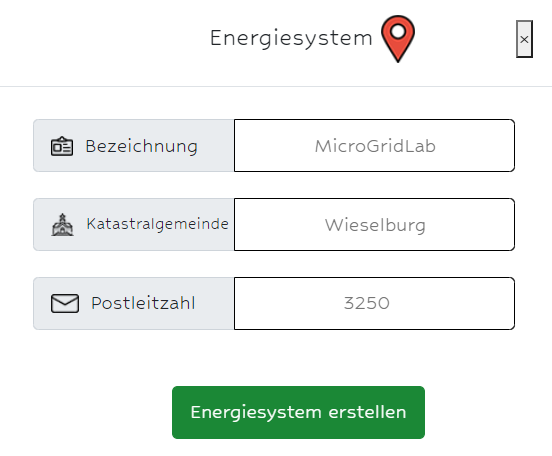
\includegraphics[height=8cm,width=9cm]{images/ESerstellenPop}
	\caption{Energiesystem erstellen Pop-up}
	\label{fig:ESerstellenPopup}
\end{figure}
\newpage
Die Attribute Längengrad und Breitengrad werden automatisch mithilfe des Mausklicks auf der Karte mit den entsprechenden Koordinaten beim Erstellen des Energiesystems befüllt. Das Attribut User\_ID wird automatisch mit der ID des gerade angemeldeten Benutzers ausgefüllt, um das Energiesystem einem Benutzer zuteilen zu können.
\newline
Nachdem der Benutzer alle Daten eingegeben hat, werden diese Daten an den Controller übermittelt, wo anschließend das Energiesystem erstellt und in der Datenbank erfasst wird. Das Ergebnis ist eine Datenbankabfrage aller vorhandenen Energiesysteme, welche zurück an die Weboberfläche übergeben werden, um die Energiesysteme-Marker auf der Karte zu platzieren sowie den Inhalt der Liste aller vorhandenen Energiesysteme zu aktualisieren.  
Die folgende \autoref{fig:Eserstellendiagramm} zeigt den Ablauf, um ein Energiesystem zu erstellen.

\begin{figure}[h]
	\centering
	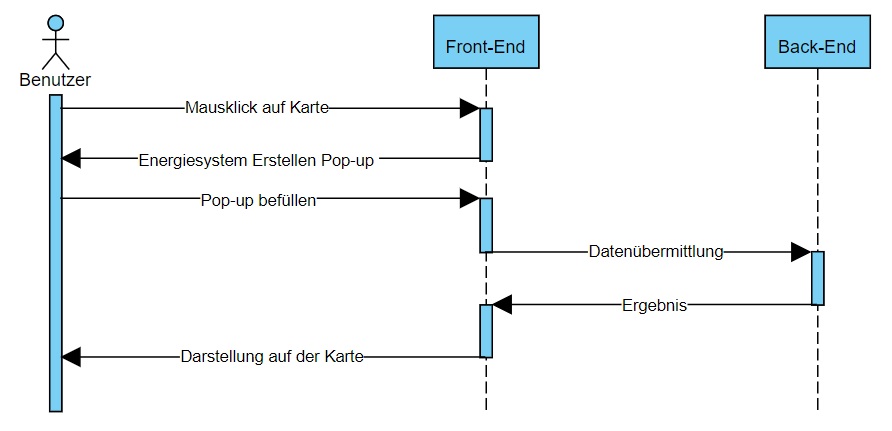
\includegraphics[height=7cm,width=14cm]{images/ESerstellen}
	\caption{Energiesystem erstellen}
	\label{fig:Eserstellendiagramm}
\end{figure}





\subsubsection{Energiesystem bearbeiten}
Mit dem Stift-Icon beim Energiesystem in der Liste ist es möglich, die Kerndaten eines Energiesystems zu bearbeiten. Die zu bearbeitenden Daten, welche einen weißen Hintergrund  aufweisen, lauten auf „Bezeichnung“, „Katastralgemeinde“ und „Postleitzahl“. Die Koordinaten sowie die User\_ID des Energiesystems bleiben konstant und sind nicht änderbar und nicht im Pop-up ersichtlich.
Folgende weitere Attribute werden bei jedem Energiesystem automatisch berechnet, angezeigt und sind nicht bearbeitbar, sondern dienen nur als weitere Information über das ausgewählte Energiesystem. 
\begin{itemize}
	\item Anzahl-Erzeugungstechnologien  
	\item Anzahl-Verbraucher
	\item Anzahl-Speicher
	\item Ges-Nennleistung [kW]
	\item Ges-Energie [kW/h]
	\item Ges-Verbraucher-Leistung [kW]
	\item Ges-Verbraucher-Energie [kW/h]
	\item Ges-Erzeuger-Leistung [kW]
	\item Ges-Erzeuger-Energie [kW/h]
	\item Ges-Speicher-Kapazität [kW/h]
	\item Aktueller Netzbezug [kW]
\end{itemize}
Für genauere Informationen zu den einzelnen Attributen siehe Kapitel  \ref{sec:Verwendete Icons und deren Bedeutungen}.
Mit dem Button „Mehr Details zu diesem Energiesystem“ ist es möglich, die weiteren Daten des Energiesystems ein- und auszuklappen. 
Das Pop-up zum Bearbeiten eines Energiesystems ist in der \autoref{fig:ESbearbeitenPop} ersichtlich.
\begin{figure}[h]
	\centering
	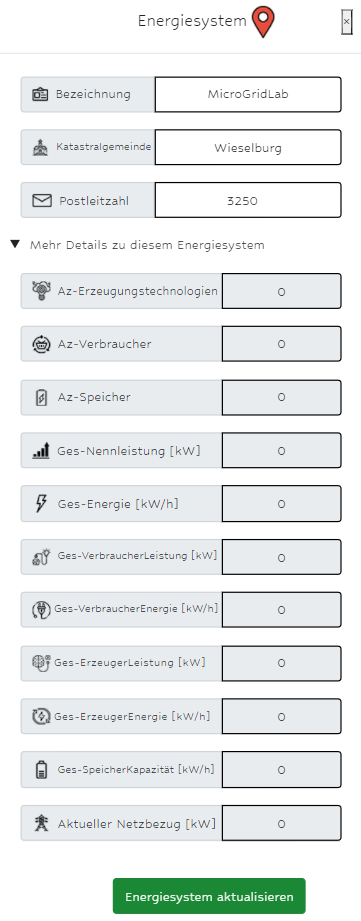
\includegraphics[height=9cm,width=9cm]{images/ESbearbeitenPop}
	\caption{Energiesystem bearbeiten Pop-up}
	\label{fig:ESbearbeitenPop}
\end{figure}

Nachdem der Benutzer die Attribute des Energiesystems bearbeitet hat, werden diese mithilfe des Controllers in der Datenbank aktualisiert. Anschließend werden die neuen Daten der Weboberfläche übergeben, um auf der Karte sowie in der Liste den aktuellen Stand der Energiesysteme darstellen zu können. Der Ablauf der dieser Funktion ist gleichzusetzen mit dem Ablauf der Energiesystem Erstellen Funktion, mit dem Unterschied, dass sich das Bearbeiten Pop-up öffnet um die Daten des Energiesystems zu bearbeiten. Dieser Ablauf ist in der \autoref{fig:Eserstellendiagramm} ersichtlich.


\newpage
\subsubsection{Energiesystem löschen}
Um ein Energiesystem zu löschen, benötigt man das Mülleimer-Icon, welches sich neben jedem Energiesystem in der Liste befindet, sofern der angemeldete Benutzer die erforderliche Berechtigung dazu hat. 
Nachdem dieses Icon betätigt wurde, wird die Information, dass ein Energiesystem gelöscht wurde, an den Controller übermittelt. Dieser löscht anschließend mithilfe der ID des ausgewählten Energiesystems dieses aus der Datenbank und übergibt alle anderen Energiesysteme zurück auf die Weboberfläche, um die vorhandenen Energiesysteme auf der Karte zu platzieren sowie in der Liste anzuzeigen. 
 
 
\subsubsection{Energietechnologie erstellen}
Für das Erstellen einer Energietechnologie ist das Auswählen eines Energiesystems mit einem Doppelklick notwendig. Anschließend verwandelt sich der Cursor in das Energietechnologie-Icon, welches darauf hindeutet, dass jetzt das Hinzufügen einer Energietechnologie mittels eines Klicks auf der gewünschten Position auf der Karte möglich ist. Nach dem Klick auf der Karte öffnet sich ein Pop-up-Fenster, um die Kerndaten der Energietechnologie einzugeben. Dieses Pop-up ist in der \autoref{fig:EterstellenPop} ersichtlich. 


Eingabe des Benutzers:
\begin{itemize}
	\item Bezeichnung 
	\item Typ
	\item Ort
	\item Bild einfügen
	\item Beschreibung
\end{itemize}

Automatisch ausgefüllt und nicht im Pop-up dargestellt:
\begin{itemize}
	\item Längengrad 
	\item Breitengrad
	\item Ensys\_ID
	\item User\_ID
\end{itemize}
\begin{figure}[h]
	\centering
	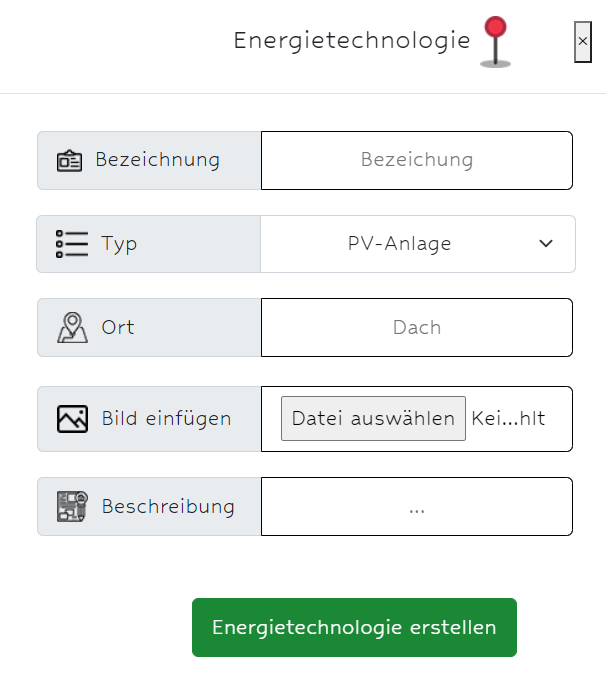
\includegraphics[height=8cm,width=7cm]{images/ETerstellenPop}
	\caption{Energietechnologie erstellen Pop-up}
	\label{fig:EterstellenPop}
\end{figure}
\newpage
Nachdem der Benutzer die Daten im Pop-up ausgefüllt hat, werden diese Informationen über den Controller in der Datenbank erfasst. Anschließend werden die Energietechnologie-Daten an die Weboberfläche übermittelt, um die Energietechnologien auf der Karte darzustellen sowie in der Liste anzuzeigen. Der Ablauf, um eine Energietechnologie zu erstellen, wird in der \autoref{fig:Eterstellendiagram} dargestellt:
 \begin{figure}[h]
 	\centering
 	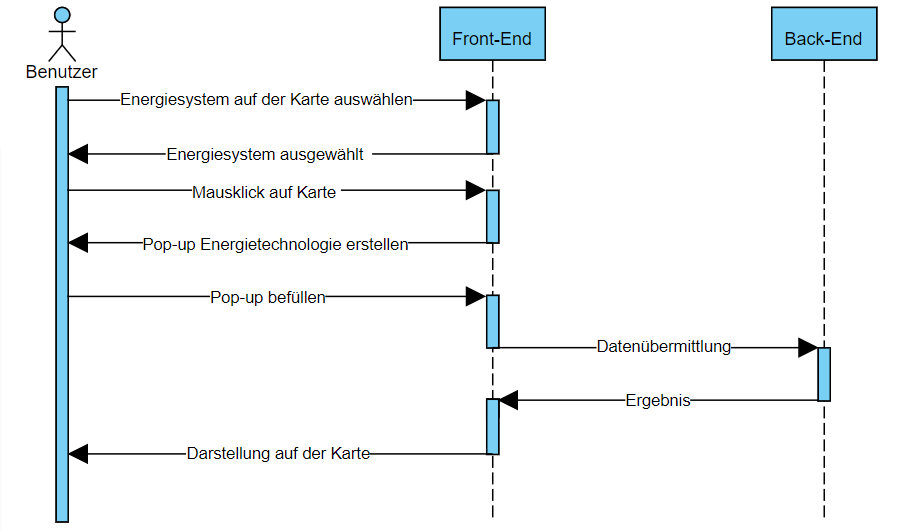
\includegraphics[height=7cm,width=14cm]{images/ETerstellen}
 	\caption{Energietechnologie erstellen}
 	\label{fig:Eterstellendiagram}
 \end{figure}

\newpage
\subsubsection{Energietechnologie bearbeiten}
Um eine Energietechnologie zu bearbeiten, muss zuerst ein Energiesystem mit einem Doppelklick ausgewählt werden. Anschließend befinden sich rechts in der Liste alle dazugehörigen Energietechnologien, welche man mit dem Stift-Icon bearbeiten kann. Nach dem Betätigen des Stift-Icons öffnet sich ein Pop-up-Fenster, um die Attribute zu bearbeiten. Dieses Pop-up-Fenster ist in der \autoref{fig:ETbearbeitenpop} ersichtlich.
\newline
\begin{figure}[h]
	\centering
	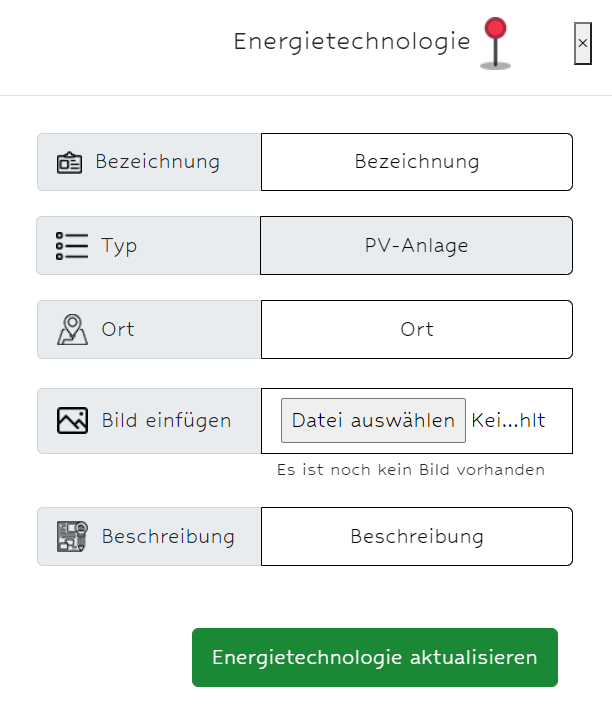
\includegraphics[height=11cm,width=8cm]{images/ETbearbeitenPop}
	\caption{Energietechnologie bearbeiten}
	\label{fig:ETbearbeitenpop}
\end{figure}


Dabei sind die Attribute „Bezeichnung“, „Ort“, „Bild“ und „Beschreibung“ bearbeitbar. Um dem Benutzer dies deutlich zu machen, weisen diese Attribute einen weißen Hintergrund auf. 
Die Attribute „Typ“, „Längengrad“, „Breitengrad“, „Ensys\_ID“ sowie „User\_ID“ sind nicht bearbeitbar.
Nachdem der Benutzer die Daten bearbeitet hat, werden diese über den Controller in die Datenbank geschrieben. Anschließend werden die Energietechnologie-Daten an die Weboberfläche übergeben, um die Marker auf der Karte zu platzieren sowie den Inhalt der Liste zu aktualisieren. Der Ablauf der dieser Funktion ist gleichzusetzen mit dem Ablauf der Energietechnologien Erstellen Funktion, mit dem Unterschied, dass sich das Bearbeiten Pop-up öffnet um die Daten der Energietechnologie zu bearbeiten. Dieser Ablauf ist in der \autoref{fig:Eterstellendiagram} ersichtlich. 


\newpage
\subsubsection{Energietechnologie löschen}
Um eine Energietechnologie zu löschen, benötigt man das Mülleimer-Icon, welches sich in der Liste neben den Energietechnologien befindet, sofern ein Energiesystem von dem Benutzer ausgewählt wurde.
Sobald der Benutzer dieses Icon betätigt, wird mithilfe der ID der ausgewählten Energietechnologie dem Controller mitgeteilt, dass diese Energietechnologie gelöscht werden soll. Daraufhin löscht der Controller diese Energietechnologie aus der Datenbank und übergibt anschließend alle anderen vorhandenen Energietechnologie-Daten an die Weboberfläche, um dort die Marker zu platzieren sowie den Inhalt der Liste zu aktualisieren.


\subsubsection{Benutzerverwaltung}
Je nach Benutzerrolle des aktuell angemeldeten Benutzers stehen dem Benutzer unterschiedliche Funktionen auf der Weboberfläche zur Verfügung.  
Folgende drei Rollen stehen zur Verfügung:
\begin{itemize}
	\item Administrator 
	\item Mitarbeiter
	\item Öffentlicher Benutzer
\end{itemize}
Wie eine generelle Überprüfung des Benutzers in Laravel umgesetzt werden kann, ist unter der Quelle x.y ersichtlich. 
\newline Folgende Überprüfung wurde selbst vom Projektteam entwickelt und ist somit nicht unter der genannten Quelle auffindbar.\newline \newline
Mit dieser Überprüfung wird kontrolliert, ob der gerade angemeldete Benutzer das Energiesystem oder die Energietechnologie selbst erstellt hat oder ob er die Rolle des Administrators aufweisen kann. Falls der Benutzer das Energiesystem oder die Energietechnologie selbst erstellt hat, ist der erste Teil der Überprüfung erfüllt und der Benutzer hat die Verwaltungsfunktionen zur Verfügung. Falls der Benutzer das Energiesystem oder die Energietechnologie nicht selbst erstellt hat, wird die zweite Überprüfung durchgeführt, welche überprüft, ob der Benutzer die Rolle des Administrators aufweisen kann. Falls er diese Rolle besitzt, hat er die Verwaltungsfunktionen zur Verfügung, andernfalls nicht.


\begin{lstlisting}[
	caption={Überprüfung der Benutzerrolle},
	label=Code,
	language=octave,
	numbers=left,
	firstnumber=1,
	numberfirstline=false,
	backgroundcolor=\color{mygray},
	basicstyle=\footnotesize=15,
	keywordstyle=\color{blue}
	]
@if ($userID->id == $d->users_idusers || $userID->role == 'Admin')

\end{lstlisting}


\newpage
\subsubsection{Adresssuche}
Mithilfe des Adresssuchfeldes ist es möglich, einen Standort einzugeben, um anschließend auf der Karte zu diesem zu gelangen. Dadurch ist das Auffinden von bestimmten Orten auf der Karte problemlos möglich. Dabei wird die eingegebene Adresse in geografische Koordinaten umgewandelt, zu welchen man anschließend navigiert wird. In der folgenden \autoref{fig:Adresssuchfeld} ist das Adresssuchfeld ersichtlich.
\begin{figure}[h]
	\centering
	
\includegraphics[height=2cm,width=15cm]{images/Adresssuchfeld}
	\caption{Adresssuchfeld}
	\label{fig:Adresssuchfeld}
\end{figure}

Folgende Schreibweisen sind in der Suche möglich:
\begin{itemize}
	\item Stadt 
	\item Land
	\item Straße 
	\item Postleitzahl 
\end{itemize}


\textbf{Automatische Vervollständigung} \\
Um die Suche nach der richtigen Adresse zu vereinfachen, wird die Eingabe des Benutzers mit einer Autocomplete-Funktion unterstützt. Diese Funktion bietet mögliche Ziel-Adressen anhand der bisher eingegebenen Daten an, welche vom Benutzer ausgewählt werden können. Dafür wurde eine von Google bereitgestellte API verwendet. 
Quelle Xy 
Ein Beispiel dieser Funktion ist in der \autoref{fig:Automatische Vervollständigung} dargestellt.

\begin{figure}[h]
	\centering
	\includegraphics[height=7cm,width=15cm]{images/Vorschläge}
	\caption{Automatische Vervollständigung}
	\label{fig:Automatische Vervollständigung}
\end{figure}

\newpage
\textbf{Adresssuche durchführen} \\
Die Adresssuche kann auf zwei verschiedene Arten ausgelöst werden.
Die erste Variante ist das Benutzen des dazugehörigen Buttons mit der Beschriftung „Suchen“. Die zweite Variante ist das Betätigen der Enter-Taste auf der Tastatur. Beide Varianten führen zu dem gleichen Ergebnis, und zwar, dass die Adresssuche durchgeführt wird.
Sobald die Adresssuche durchgeführt wird, werden mit Hilfe von Google-Cloud API-Aufrufe für die eingegebene Adresse die dazugehörigen Koordinaten berechnet. Sobald diese berechnet wurden, werden diese an die Karte übergeben, damit der Mittelpunkt der Karte auf diese Koordinaten gesetzt wird. Anschließend gelangt der Benutzer zu seiner eingegebenen Adresse auf der Karte und kann seine Interaktionen fortsetzen. Die \autoref{fig:AdresseDiagramm} beschreibt die Durchführung der Adresssuche.
\begin{figure}[h]
	\centering
	\includegraphics[height=7cm,width=17cm]{images/Adresssuche}
	\caption{Adresssuche}
	\label{fig:AdresseDiagramm}
\end{figure}



\newpage
\subsection{Front-End} \label{sec: Front-End}
Das Projektteam hat sich bei der Front-End Gestaltung an die Vorgabe des Auftraggebers gehalten und sich an der bereits vorhanden Website der Best GmbH, welche in \ref{fig:Website Best GmbH} ersichtlich ist, orientiert. Das Produkt wurde dann mithilfe der Laravel Layout\footnote{genauer in \autoref{sec: Layout} erklärt }Funktion in Header Footer und Content unterteilt.Generell ist das Produkt gegliedert in folgende Unterseiten: 
\begin{itemize}
	\item Home 
	\item Energiesysteme
	\item Galerie 
	\item Impressum 
	\item Datenschutz
	\item Registrierungsseite
\end{itemize}
Auf die oben aufgezählten Unterseiten wird in den nachfolgenden Kapiteln genauer eingegangen.
\begin{figure}[h]
	\centering
	\includegraphics[height=7cm,width=15cm]{images/BestGmbHSeite}
	\caption{Website Best GmbH}
	\label{fig:Website Best GmbH}
\end{figure}
\newpage

\subsubsection{Home}
Die Homeseite ist die erste Seite, die ein Benutzer zu Gesicht bekommt, wenn er das Produkt aufruft. Die Seite besteht aus einer Diashow, die Bilder des Micro Grid Lab Projekts der Best GmbH zeigt. Unter dieser befindet sich ein Textbereich, auf welchem das Projekt “Micro Grid Lab” kurz vorgestellt wird. Hier ein Bild der besagten Seite:
\begin{figure}[h]
	\centering
	\includegraphics[height=7cm,width=14cm]{images/HomeSeite1}
	\caption{Oberer Teil der Home Seite}
	\label{fig:HomeSeite1}
\end{figure}
\begin{figure}[h]
	\centering
	\includegraphics[height=7cm,width=14cm]{images/HomeSeite2}
	\caption{Unterer Teil der Homeseite}
	\label{fig:HomeSeite1}
\end{figure}
\newpage
\subsubsection{Energiesysteme}
Die Energiesystemeseite ist die Seite, wo die Hauptfunktion des Produkts verwendet werden kann. Auf dieser wird die Verwaltung der Energiesysteme und Energietechnologien mithilfe einer Map visuell dargestellt. Diese Seite besteht aus einer Google Maps Karte, welche sich auf der linken Seite der Website befindet. Ebenso einem DataTable auf der rechten Hälfte der Website. Hier ein Bild der eben beschriebenen Seite:
\begin{figure}[h]
	\centering
	\includegraphics[height=6cm,width=14cm]{images/EnergiesystemSeite}
	\caption{Die Energiesystem Seite}
	\label{fig:Energiesystem Seite}
\end{figure}

\subsubsection{Galerie}
Das Produkt bietet auch die Möglichkeit, zu jeder Energietechnologie ein dementsprechendes Bild zu speichern. Dieses Bild wird dann in der Bildergalerie angezeigt. Durch einen Dropdown, welches sich oben in der Mitte der Seite befindet, kann ein Energiesystem auswählt werden. Von diesem ausgewählten Energiesystem werden dann alle dazugehörigen Energietechnologien mit dem entsprechendem Bild angezeigt. Die Galerie sieht folgendermaßen aus:
\begin{figure}[h]
	\centering
	\includegraphics[height=6cm,width=14cm]{images/GalerieSeite}
	\caption{Die Galerie}
	\label{fig:Galerie}
\end{figure}


\subsubsection{Impressum}
Auf der Impressumsseite, welche durch den Footer erreichbar ist, ist das Impressum der Website einsehbar. Die Seite hat eine Überschrift  “Impressum” und darunter befindet sich ein Textbereich  mit dem dazugehörigen Impressum. Am Ende des Impressums befindet sich noch ein Link, welcher auf die Homepage der Best GmbH weiterleitet. Hier ist ein Foto der Impressumsseite:

\begin{figure}[h]
	\centering
	\includegraphics[height=6cm,width=14cm]{images/ImpressumSeite}
	\caption{Das Impressum}
	\label{fig:Impressum}
\end{figure}

\subsubsection{Datenschutz}
Wie auch die Impressumsseite ist die Datenschutzseite durch den Footer erreichbar. Diese ist gleich aufgebaut wie die Impressumsseite. Auch hier gibt es wieder mittig eine Überschrift “Datenschutz”, unter welcher wieder ein Textbereich vorhanden ist. In diesem Textbereich  ist die Datenschutzgrundverordnung des Produkts einsehbar.  Hier ein Foto der Datenschutzseite:
\begin{figure}[h]
	\centering
	\includegraphics[height=6cm,width=14cm]{images/DSGVOSeite}
	\caption{Die Datenschutzseite}
	\label{fig:DSGVO}
\end{figure}
\subsubsection{Registrierungsseite}
Die Registrierungsseite kann nur von einem Administrator erreicht werden. Auf dieser Seite ist es möglich, neue Benutzer zu registrieren oder bereits vorhandene Benutzer zu löschen. Genauere Informationen zu dieser Seite sind im Kapitel 3.5.3 nachlesbar. Hier ein Foto der Registrierungsseite:
\begin{figure}[h]
	\centering
	\includegraphics[height=7cm,width=14cm]{images/RegisterSeite}
	\caption{Die Registrierungsseite }
	\label{fig:RegisterSeite}
\end{figure}



\subsection{Login}
Möchte sich ein Benutzer beim Produkt anmelden, kann er dies beim Loginfeld, welches in  Abbildung \ref{fig:LoginFormular} ersichtlich ist. Dort meldet er sich mit einer E-Mail-Adresse und einem Passwort an, welche vorher auf der Registrierungsseite angelegt wurde. Nach Eingabe der Daten, wird überprüft, ob die Daten in der Datenbank vorhanden sind und das Passwort richtig eingegeben wurde. Das Loginfeld sieht folgendermaßen aus:

\begin{figure}[h]
	\centering
	\includegraphics[height=5cm,width=7cm]{images/LoginFeld}
	\caption{Das Login Formular}
	\label{fig:LoginFormular}
\end{figure}

\subsection{Registrierung}
Um neue Benutzer registrieren zu können, gibt es eine eigene Registrierungsseite. Diese Seite, ersichtlich in Abbildung xy Registrierungsseite, besteht aus einem Formular und einem DataTable und kann nur von Benutzern mit der Rolle Admin aufgerufen werden. Auf dem DataTable werden alle vorhandenen Benutzer angezeigt. Des Weiteren bietet er die Möglichkeit, vorhandene Benutzer zu löschen. Das Formular ermöglicht es, Benutzer mit folgenden Werten anzulegen:
\begin{itemize}
	\item Name  
	\item E-Mail-Adresse
	\item Passwort  
	\item Rolle 
\end{itemize}
\begin{figure}[h]
	\centering
	\includegraphics[height=3cm,width=5cm]{images/RegisterFormular}
	\caption{Das Registrierungsformular}
	\label{fig:Register Formular}
\end{figure}



\subsection{Kartendienst Funktionalitäten}
Neben den bekannten Kartendienst-Funktionen wie das Erstellen eines Energiesystems oder einer Energietechnologie bietet die Karte weitere Funktionen. Diese weiteren Funktionen sind das Auswählen und Abwählen eines Energiesystems.

\subsubsection{Auswählen eines Energiesystems}
Das Auswählen eines Energiesystems ist notwendig, um die dazugehörigen Energietechnologien auf der Karte sowie in der Liste zu sehen. Ebenso ist es notwendig, um neue Energietechnologien erstellen zu können.
Mit einem einfachen Klick auf das Energiesystem-Icon wird an dieses Energiesystem lediglich herangezoomt, jedoch noch nicht ausgewählt.
Um ein Energiesystem auszuwählen, ist ein Doppelklick darauf notwendig. Dieser Doppelklick bewirkt, dass in der Liste sowie auf der Karte die dazugehörigen Energietechnologien angezeigt werden. Anschließend ist es für den Benutzer möglich, die Energietechnologien zu verwalten. Der Ablauf für das Auswählen eines Energiesystems wird in der \autoref{fig:Energiesystem auswählen} dargestellt:
\newline
\begin{figure}[h]
	\centering
	\includegraphics[height=7cm,width=14cm]{images/ESauswählen}
	\caption{Energiesystem auswählen}
	\label{fig:Energiesystem auswählen}
\end{figure}


\subsubsection{Abwählen eines Energiesystems}
Nachdem ein Energiesystem ausgewählt wurde, ist mit einem einfachen Linksklick auf das Energiesystem-Icon möglich, das ausgewählte Energiesystem wieder abzuwählen. Nach Abwählen des Energiesystems werden die dazugehörigen Technologien wieder von der Karte sowie aus der Tabelle entfernt. Stattdessen werden in der Tabelle wieder alle vorhandenen Energiesysteme angezeigt.



\newpage
\subsection{Anzeige von Energiesystemen und Energietechnologien auf der Karte}
In diesem Abschnitt werden die Funktionen zum Darstellen und Entfernen der Marker auf der Karte erläutert.



\subsubsection{Energiesysteme Marker auf der Karte platzieren}
Immer wenn die Map neu geladen wird, werden alle vorhandenen Energiesysteme in Form von Icons auf der Karte platziert. Dafür werden die Daten aller Energiesysteme aus der Datenbank gelesen, um anschließend die Marker auf der Karte platzieren zu können. Die dafür notwendigen Datenbank-Attribute, die ausgelesen werden müssen, sind „Bezeichnung“, „Breitengrad“ sowie „Längengrad“. Anschließend werden mit diesen Informationen die Marker erstellt und auf der Karte dargestellt. Die \autoref{fig:ETmarkerplatzieren} beinhaltet den Ablauf für das Platzieren der Energiesysteme-Marker auf der Karte.


\subsubsection{Energietechnologien Marker auf der Karte platzieren}
Sobald ein Energiesystem ausgewählt wurde, werden die dazugehörigen Energietechnologien angezeigt. Für das Anzeigen eines Energietechnologie-Markers werden die Attribute „Bezeichnung“, „Typ“, „Breitengrad“ sowie „Längengrad“ aus der Datenbank ausgelesen. Anschließend werden die Energietechnologie-Marker erstellt und auf der Karte präsentiert. Die \autoref{fig:ETmarkerplatzieren} stellt den Ablauf für das Platzieren der Energietechnologien-Marker auf der Karte dar.
\newline
\begin{figure}[h]
	\centering
	\includegraphics[height=7cm,width=14cm]{images/SetETMarker}
	\caption{Energietechnologie Marker platzieren}
	\label{fig:ETmarkerplatzieren}
\end{figure}

\newpage
\subsection{Layoutvorlage der Website}
Das Produkt verwendet die Layout Funktion vom Framework Laravel. Genauer Informationen wie dieses Layout funktioniert können im \autoref{sec: Layout} nachgelesen werden. Jede Unterseite des Produkts ist in folgende Sections gegliedert:
\begin{itemize}
	\item Header  
	\item Content
	\item Footer  
\end{itemize}

In der Section Header ist die Navigationsleiste vordefiniert. Die Section Content ist leer, da hier der individuelle Inhalt der einzelnen Unterseiten hineinkommt. In der Section Footer wurde ein selbst erstellter Footer eingefügt.




\section{DataTable} \label{sec:DataTable}
Um die angezeigten Daten in der Tabelle zu sortieren, zu filtern oder deren Anzahl pro Seite zu begrenzen, wurde das Plug-in DataTable verwendet. DataTable ist ein Plug-In der JavaScript-Bibliothek jQuery. Dieses Tool bietet viele Funktionen wie die Suchfunktion, die Sortierfunktion und die Seitennummerierung.

Das Projektteam hat sich für eine Einbindung mittels CDN \footnote{Content Delivery Network Quelle x}  entschieden.
Für einen Standard-DataTable mittels CDN sind folgende Schritte notwendig:

JavaScript und CSS-Files einbinden
\newline Je nach Verwendungsart des DataTables müssen unterschiedliche JavaScripts und CSS-Files eingebunden werden. Unter der  Quelle x.y kann herausgefunden werden, welche Files eingebunden werden müssen. 

Nachdem die Files eingebunden sind, muss folgende Funktion hinzugefügt werden.
\definecolor{mygray}{RGB}{252,251,244}
\renewcommand{\lstlistingname}{Quellcode}

\begin{lstlisting}[
	caption={DataTable Funktion},
	label=Code,
	language=octave,
	numbers=left,
	firstnumber=100,
	numberfirstline=false,
	backgroundcolor=\color{mygray},
	basicstyle=\footnotesize=15,
	keywordstyle=\color{blue}
	]
$(document).ready( function () {
	$('#TableID).DataTable();
} );

	
\end{lstlisting}

Anschließend sind alle DataTable-Funktionen an diesen Table gegeben.
Links oben befindet sich ein Input-Feld, um die Anzahl der Datensätze pro Seite festzulegen. Die Suchfunktion, um nach einem bestimmtem Datensatz zu suchen, befindet sich rechts oben.
Für jedes Attribut ist eine Sortierfunktion gegeben, welche an den kleinen Pfeilen neben dem Attributnamen erkennbar ist. Links unten sieht man, wieviele Datensätze gerade auf dieser Seite angezeigt werden und wieviele es insgesamt gibt. Rechts unten ist es möglich, mit den Buttons zwischen den Seiten hin und her zu wechseln, falls mehrere Seiten vorhanden sind.
Die Sprache, die für den Standard-DataTable verwendet wird, ist Englisch.
In der \autoref{fig:StandardTable} ist ein DataTable mit den Standardeinstellungen ersichtlich.
\newline
\begin{figure}[h]
	\centering
	\includegraphics[height=5cm,width=10cm]{images/DataTableStandard}
	\caption{Standard DataTable}
	\label{fig:StandardTable}
\end{figure}


\subsection{Individueller DataTable}
Aufbauend auf den Standard-DataTable wurde der individuelle DataTable basierend auf den Anforderungen des Auftraggebers erstellt. Dabei ist die wichtigste Anforderung, dass pro Seite maximal 5 Datensätze dargestellt werden.
Zuerst wurde die Sortierfunktion bei den Spalten drei, vier und fünf deaktiviert, da sich an diesen Stellen die Icons befinden und somit eine Sortierfunktion keinen Sinn macht. Die Auswahl für die Anzahl der Datensätze pro Seite wurde deaktiviert, da diese konstant auf den Wert fünf festgelegt wurde. Zum Schluss wurde die Sprache des Tables auf Deutsch geändert.
In der \autoref{fig:indiTable} ist der individuelle DataTable abgebildet.
\begin{figure}[h]
	\centering
	\includegraphics[height=5cm,width=10cm]{images/DataTableIndividuell}
	\caption{Individueller DataTable}
	\label{fig:indiTable}
\end{figure}




\subsection{Sortierfunktion}
Mit der Sortierfunktion ist es möglich, nach jedem einzelnen Attribut in der Liste zu sortieren. Die Sortierfunktion ist nur bei jenen Attributen aktiviert, wo es auch Sinn macht. Somit ist die Sortierfunktion bei den Icons nicht gegeben. Beim Laden des Tables ist der Inhalt automatisch alphabetisch nach dem ersten Attribut sortiert. Nach dem Betätigen der Sortierfunktion wird anschließend alphabetisch rückwärts sortiert.  


\subsection{Suchfunktion}
Die Suchfunktion ermöglicht eine sofortige Textsuche des Inhaltes in der Liste. Dabei ist es möglich, mit Buchstaben oder mit Zahlen zu suchen. Jeder Datensatz, der den eingegebenen Buchstaben oder die eingegebene Zahl beinhaltet, wird angezeigt. Der Rest wird ausgeblendet und ist erst nach dem Beenden der Suche wieder sichtbar.


\subsection{Seitenanzahl}
Wenn auf einer Seite maximal fünf Datensätze angezeigt werden, entstehen bei einer großen Anzahl von Energiesystemen sowie Energietechnologien entsprechend viele Seiten. Diese Seiten sind mithilfe der Buttons rechts unten navigierbar. Links unten steht die Information darüber, wieviele Seiten es insgesamt gibt, und wieviele Einträge von allen vorhandenen gerade auf dieser Seite angezeigt werden.


\subsection{Icons}
Die Verwaltung der einzelnen Energiesysteme und der Energietechnologien ist mit den dazugehörigen Icons möglich. Welche Icons zu jedem Energiesystem oder jeder Energietechnologie zur Verfügung stehen, hängt von den Rechten des angemeldeten Benutzers ab.
Es gibt zwei verschiedene Kombinationen von verfügbaren Icons.
Entweder man hat nur das Icon „Auge“ zur Verfügung, welches bedeutet, dass man dieses Energiesystem oder diese Energietechnologie entweder nicht erstellt hat, nicht mit einem Administrator-Benutzer angemeldet ist oder gerade nicht auf der Weboberfläche angemeldet ist. Mit diesem Icon hat man die Möglichkeit, die Kerndaten eines Systems zu sehen, welche aber nicht bearbeitet werden können.
Die zweite Variante ist, dass man die Icons „Mülleimer“, „Statistik“ und „Stift“ zur Verfügung hat, was bedeutet, dass der angemeldete Benutzer dieses System erstellt hat oder die Administrator-Berechtigungen besitzt. 
Auf Funktionen der einzelnen Icons wird im Kapitel 2.6.6.9 genauer eingegangen.



\subsection{MoveToMarker}
Um das Finden eines Energiesystems trotz des bereits vorhandenen Adress-Suchfeldes noch leichter zu ermöglichen, gibt es die Funktion MoveToMarker. Diese Funktion wird dann ausgeführt, wenn in der Liste auf die Bezeichnung, die Katastralgemeinde oder die Postleitzahl eines Energiesystems gedrückt wird. Das Ergebnis dieser Funktion ist, dass der Benutzer nach dem Klick auf ein Energiesystem in der Liste gleich zu dessen Position auf der Karte gelangt, um eine längere Suche danach zu ersparen. Der Ablauf der MoveToMarker-Funktion wird in der \autoref{fig:Movetomarker} nähergebracht.

\begin{figure}[h]
	\centering
	\includegraphics[height=7cm,width=14cm]{images/MoveToMarker}
	\caption{MoveToMarker}
	\label{fig:Movetomarker}
\end{figure}

Nachdem der Benutzer zum Standort des ausgewählten Energiesystems navigiert wurde, hat dieser dort wieder alle Funktionalitäten der Karte, wie das Hinzufügen eines neuen Energiesystems sowie einer Energietechnologie, gegeben.


\newpage
\section{Galerie Funktionen}
Auf der Seite „Galerie“ ist es möglich, die Energietechnologien von einem ausgewählten Energiesystem anzeigen zu lassen. Dabei steht das ausgewählte Bild beim Erstellen einer Energietechnologie im Vordergrund. Dieses wird in Form einer Card mit deren Bezeichnung und Beschreibung präsentiert.


\subsection{Auswahl eines Energiesystems}
Die Auswahl eines Energiesystems ist mithilfe eines Drop-Down-Menüs möglich. Dieses Drop-Down-Menü beinhaltet alle vorhanden Energiesysteme. In \autoref{fig:DropDowngalerie} ist das Drop-Down-Menü mit allen vorhandenen Energiesystemen ersichtlich.
\begin{figure}[h]
	\centering
	\includegraphics[height=4cm,width=14cm]{images/GalerieDropDown}
	\caption{Auswahl eines Energiesystems}
	\label{fig:DropDowngalerie}
\end{figure}


\newpage
\subsection{Energietechnologien des Energiesystems anzeigen}
Wenn der Benutzer ein Energiesystem ausgewählt hat, werden die dazugehörigen Energietechnologien in Form von Cards dargestellt.
Als Haupt-Überschrift über alle Energietechnologien dient die Bezeichnung des ausgewählten Energiesystems.
Bei den einzelnen Energietechnologien, die dargestellt werden, wird zuerst das eingefügte Bild angezeigt, welches beim Erstellen einer Energietechnologie ausgewählt werden kann. Falls der Benutzer bei einer Energietechnologie kein Bild hinzugefügt hat, wird automatisch ein Standardbild eingefügt. Unter dem Bild dient die Bezeichnung sowie die Beschreibung der Energietechnologie als Bildunterschrift. In der \autoref{fig:ETgalerie} sind Energietechnologien des Energiesystems MicroGridLab zu sehen.

\begin{figure}[h]
	\centering
	\includegraphics[height=8cm,width=14cm]{images/GalerieET2}
	\caption{Galerie}
	\label{fig:ETgalerie}
\end{figure}


\newpage
\section{Grafana}
In diesem Kapitel wird das automatische Erstellen von Dashboards via der Grafana HTTP API beschrieben. 

\subsection{Automatisches Erstellen der Dashboards} \label{sec: Dashboard}
Sobald in der Benutzeroberfläche ein Energiesystem erstellt wird, werden die Daten an die “store” Methode im “EnSysController” weitergereicht in welcher der API Aufruf zum Erstellen eines Dashboards getätigt wird. Hierzu werden die Daten welche vom Benutzer eingegeben wurden in das “json” Grundgerüst eingesetzt, welches dann an die API gesendet wird. Grafana setzt auf eine Bereichsverwaltung mit sogenannten “Organisations”, das Produkt erstellt die Dashboards und in diesen enthaltenen Panels in der sogenannten “annonymus organisation”. Diese Organisation ist von jedem einsehbar und erfordert keine Benutzerauthentifizierung. 
\begin{figure}[h]
	\centering
	\includegraphics[height=7cm,width=14cm]{images/DashboardErstellen}
	\caption{Dashboard erstellen}
	\label{fig:DashboardErstellen }
\end{figure}


\subsection{Automatisches Erstellen der Panels}\label{sec: Panels}
Wird in einem Energiesystem eine Energietechnologie erstellt, so werden die Daten wiederum an die Methode “store” im “EnTechController” übergeben. In dieser Methode werden alle in einem Dashboard bereits vorhandenen Panels per API Aufruf ausgelesen und in einem Array gespeichert, wird nun ein neues Panel erstellt, so wird dieses dem Array hinzugefügt und mit einem API Aufruf an Grafana gesendet. Weiters wird beim Erstellen des Panels mit hilfe einer “switch” Anweisung unterschieden um welchen Typ von Energietechnologie es sich handelt, um dann die richtige SQL Abfrage zu formulieren welche die Daten aus der Datenbank in das Panel liefert. 
\begin{figure}[h]
	\centering
	\includegraphics[height=7cm,width=14cm]{images/PanelErstellen}
	\caption{Panel erstellen}
	\label{fig:PanelErstellen }
\end{figure} 


\subsection{Energietechnologien Statistiken anzeigen}
Um nun in der Benutzeroberfläche des Produkts, die mit den API Aufrufen erstellten Grafana Statistiken anzeigen zu können ist, auf der Benutzeroberfläche ein Statistik Icon Vorhanden. Wird dieses vom Benutzer ausgewählt, so wird eine JavaScript Funktion welche die ID der Energietechnologie als Parameter hat ausgeführt. In dieser JavaScript Funktion wird ein Pop-Up Fenster aufgerufen sowie der “src” Parameter eines HTML “iframe” Elementes gesetzt. Dieses “iframe” Element wird nun in dem Pop-Up Fenster angezeigt.
\begin{figure}[h]
	\centering
	\includegraphics[height=8cm,width=14cm]{images/Statistikanzeigen}
	\caption{Statistik anzeigen}
	\label{fig:Statistikanzeigen }
\end{figure} 
\newpage



\section{Einbindung von Google Maps}
Um eine Karte zur Verwaltung und Visualisierung auf dem Produkt zu Verfügung zu stellen, hat sich das Projektteam für den Kartendienst Anbieter Google Maps entschieden. Um die Funktionen von Google Maps zu nutzen, muss ein Google Cloud Account erstellt und eingebunden werden. Was Google Cloud ist und wie es verwendet wird, ist in den nachfolgenden Kapiteln genauer erklärt.

\subsection{Google Cloud} \label{sec: Google Cloud}
Google Cloud ist die zentrale Verwaltung aller von Google bereitgestellten Cloud Dienste. Das Projektteam benötigt diese Plattform, um die Google Maps Karte in das Produkt einzubinden. In den nachfolgenden Kapiteln werden alle Schritte erklärt, die es benötigt, um das Projekt zusammen mit Google Cloud verwenden zu können.


\subsection{Google Cloud Plattform Account erstellen}
Um Zugriff auf die Google Cloud Dienste zu erlangen ist es nötig, sich ein Konto dort zu erstellen. Aufrufbar ist die Seite über den Link : https://cloud.google.com.  Um eine genaue Anleitung zu bekommen, wie man einen Account auf dieser Seite erstellt, ist im Dokument Google Maps API zu finden.

\subsection{API's aktivieren und einbinden}
Um diverse Funktionen auf der Map zu ermöglichen, werden die von Google bereitgestellten API Dienste benötigt.  Diese API Dienste müssen auf der Google Cloud Website aktiviert werden. Folgende API's werden benötigt:
\begin{itemize}
	\item Geocoding API 
	\item Javascript API
	\item Places API  
\end{itemize}
Nach Aktivierung der oben aufgezählten API's, muss ein dazugehöriger API Key erstellt werden. Dieser API Key ermöglicht es, mit dem Produkt auf die Google Cloud Dienste zuzugreifen. Auf Google Cloud sind die Keys unter der Navigier Möglichkeit  “Anmeldedaten” ersichtlich. Dort können diese auch  erstellt oder gegebenenfalls gelöscht werden. Wenn ein API Key erstellt wurde, muss dieser im Programm eingebunden werden. Er wird überall dort eingebunden, wo diese Dienste verwendet werden oder eine Anfrage an die API gesendet wird. Um genauere Informationen und eine Step by Step Anleitung zu bekommen, lesen Sie in der Datei Google Maps API nach.

\newpage
\subsection{Individuelle Map erstellen und einbinden}
Eine weitere Funktion, die von Google Cloud angeboten wird, ist das Erstellen einer eigenen Map. 
Um eine eigene Map einzurichten, muss zuerst ein Map Design erstellt werden, welches später mit der Map verknüpft wird. Das Map Design bietet die Möglichkeit, diverse Orte, Gebäude und Lokale  ein oder auszublenden. Straßen oder Straßenbezeichnungen können angezeigt oder versteckt werden. Wenn die erstellte Map mit dem richtigen Map Design verbunden ist, muss ein dazugehöriger Map Key erstellt werden. Dieser Map Key muss dann in jeder Stelle im Code eingebunden werden, wo eine Google Maps Karte initialisiert wird. Um eine Step by Step Anleitung zu bekommen, lesen Sie in der Datei Google Maps API nach.



\chapter{Resümee und Ausblick}
Die Diplomarbeit ist reibungslos verlaufen, jedoch würde das Projektteam andere Ansätze wählen bei einem Projekt gleicher Art. Die Kommunikation mit dem Auftraggeber hat sehr gut funktioniert, jedoch sind bei den laufenden Meetings immer wieder neue Änderungsvorschläge vonseiten des Auftraggebers gekommen. Dadurch entstanden für das Projektteam immer wieder neue Herausforderungen, welche zusätzlich zum definierten Projektziel umgesetzt werden sollten. Am Start der Entwicklung hatte das Projektteam mehrere Komplikationen bei der Verwendung von Git, da dabei immer wieder unerklärliche Fehler aufgetreten sind. Diese Fehler konnten jedoch mit der Zeit vom Projektteam gelöst werden, womit eine reibungslose Zusammenarbeit möglich wurde. Das Projektteam wird sich nach Abschluss der Diplomarbeit darum kümmern, die letzten Änderungsvorschläge des Auftraggebers umzusetzen. Anschließend ist das Projektteam nicht länger für das Produkt und dessen Verwaltung zuständig.


\chapter{Quellen und Literatur}

\chapter{Verzeichnisse}
\listoffigures

\listoftables

\listof{lstlisting}{Codeverzeichnis}


\chapter{Begleitprotokoll gem. § 9 Abs. 2 PrO-BHS}
Das Begleitprotokoll repräsentiert, welches Teammitglied woran und wie lange gearbeitet hat. Für das Verfassen der Begleitprotokolle wurden folgende Abkürzungen verwendet: 
\begin{itemize}
	\item Besprechung(D, A, Bu) = Besprechung mit Auftraggeber und Herrn Professor Burgstaller
		\subitem Die Buchstaben symbolisieren die Teilnehmer der Besprechung 
		\subitem D = Diplomanden
		\subitem A = Auftraggeber
		\subitem Bu = Dipl.-Ing. Johann Burgstaller
	\item SP = Sitzungsprotokoll, welches für jede Besprechung erstellt wurde
	
	
\end{itemize}

\newpage
\section{Begleitprotokoll David Pöchacker}
\begin{table}[h]
	\begin{tabular}{|l|l|l|}
		\hline
		\textbf{KW/JAHR} &     \textbf{TÄTIGKEIT}  & 	\textbf{AUFWAND (h)}    \\ \hline
		
13/21   & Erste Besprechung (D, A, Bu) & 3 	\\ \hline
17/21   & Grafische Skizze vorhandenes System  & 1 	\\ \hline
18/21   & Besprechung (D, A)  & 1 	\\ \hline
20/21   & Besprechung (D, A, Bu), Pflichtenheft erstellt & 5,5 	\\ \hline
22/21   & Besprechung (D, A, Bu), SP verfasst & 2,5 	\\ \hline
25/21   & Begleitprotokoll, Begriffserklärung Katalog, Lastenheft erstellt & 7,5   \\
		& Besprechung (D, A, Bu), SP erstellt & \\ \hline	
27/21   & Meilensteinplan erstellt, Datenbank-Schema diskutiert  & 3 \\
		& Besprechung (D, A, Bu), SP verfasst & 	\\ \hline		
28/21   & Besprechung (D, Bu) über den Meilensteinplan, Diplomarbeitsantrag erstellt  & 1,5 \\ \hline		
29/21   & Projekthandbuch, MS Project Datei, Controlling Sheet erstellt & 7,25 	\\ \hline
30/21   & Arbeitsstunden in MS Project Datei eingetragen, Besprechung (D, Bu) & 7 	\\ \hline
31/21   & Besprechung (D, A), SP verfasst  & 1	\\ \hline
32/21   & Laravel Installation und Recherche, Back-End Entwicklung (Laravel) & 4,75	\\ \hline
33/21   & Laravel Recherche, Laravel Dokumentation verfasst & 5,5	\\ \hline
34/21   & Back-End Entwicklung (Views erstellt, Datenbankverbindung, Routen) & 7,75	\\ \hline
35/21   & Back-End Entwicklung (Datensätze Erstellen, Löschen), GitHub eingerichtet  & 12 \\ 
        & Besprechung (D, Bu), SP verfasst, Kartendienst Implementierung  &	\\ \hline
36/21   & Diplomarbeitsantrag in der Datenbank befüllt, Start-Präsentation durchgeführt & 6 \\
		& Erste Design-Vorschläge verfasst & \\ \hline    
37/21   & Besprechung (D, Bu) Diplomarbeitsantrag eingereicht & 5 \\ 
		&  Design-Vorschläge verbessert &\\ \hline
38/21   & Besprechung (D, A, Bu) bezüglich Design-Vorschläge & 10 \\
		& Finalen Design-Vorschlag und Benutzerhandbuch erstellt &  \\ \hline	
39/21   & Besprechung (D, A, Bu) bezüglich finalen Design-Vorschlag, SP verfasst  & 2,5 \\
		& genaue Anforderung der Datenbankattribute und Grafana Statistiken  &  \\ \hline	
40/21   & Besprechung (D, A) & 1 \\
		& Anforderung der Datenbankattribute und Grafana Statistiken überarbeitet  &  \\ \hline	        
41/21   & Entwicklungsumgebung mit GitHub eingerichtet   & 1,5	\\ \hline
43/21   & Front-End Entwicklung (Header, Footer, Liste, Drop-Down bei Galerie Seite) & 10 \\
		& Bootstrap Recherche, CSS-Anpassungen, Icons in Photoshop angepasst   &  \\ 
		& Finale Design in Adobe XD erstellt & \\ \hline	
44/21   & Back-End Entwicklung (Energiesystem hinzufügen mit Pop-up) & 6 \\
		& Besprechung (D, A, Bu) über aktuellen Stand der Entwicklung   &  \\ \hline	     
45/21   & Google Maps Einbindung Recherche & 9,5 \\
		& Google Maps API-Dokumentation verfasst   &  \\ 
		& Google Cloud Account erstellt + Google Maps eingebunden & \\ \hline	
       
	\end{tabular}
\end{table}

\newpage
\begin{table}[h]
	\begin{tabular}{|l|l|l|}
		\hline
		\textbf{KW/JAHR} &     \textbf{TÄTIGKEIT}  & 	\textbf{AUFWAND (h)}    \\ \hline
46/21   & Back-End Entwicklung (Map-Funktionen, Funktionalitäten der Liste Icons, & 10,5 \\
		& Geo-Koordinaten werden beim Erstellen automatisch eingefügt)  &  \\ 
		& Marker Recherche, Eigene Google Map erstellt & \\ 
		& Energiesysteme-Marker aus Datenbank auslesen und auf der Karte platzieren & \\ \hline			
47/21   & Back-End Entwicklung (Authentifizierung,  & 14 \\
		& Energietechnologien eines Energiesystems anzeigen)  &  \\ 
		& Besprechung (D,A, Bu) aktuellen Stand der Entwicklung + SP verfasst & \\ 
		& Back-End Entwicklung (Energietechnologie Erstellen Funktion) & \\ \hline		
48/21   & Attribute User-ID und ES-ID wurden zu der Energietechnologie Tabelle & 2 \\
		& hinzugefügt, Funktionalitäten wieder gegeben  &  \\ \hline			
49/21   & Front-End Entwicklung (Pop-ups verschönert mit CSS) & 14,5 \\
		& Richtigen Icons der Energietechnologien auf Karte anzeigen  &  \\ 
		& Bei Energiesystem Auswahl werden die richtigen Energietechnologien angezeigt & \\ 
		& Adresssuche GeoCoding API für Autocomplete implementiert & \\ 	
		& DataTable implementiert  & \\ 
		& Karte bearbeitet (Zoom und Vollbild Button entfernt) & \\ \hline
50/21   & Besprechung (D,A, Bu) aktuellen Stand der Entwicklung + SP verfasst & 8,5 \\
& Energiesystem Pop-Up um weitere Attribute  &  \\ 
& wie Az-Energietechnologien erweitert & \\ 
& Bildergalerie wird richtiges Bild einer Energietechnologie angezeigt& \\ \hline	
51/21   & Besprechung (D,A, Bu) aktuellen Stand der Entwicklung + SP verfasst & 0,5 \\ \hline			
52/21   & Schriftliche Arbeit Inhaltsverzeichnis erstellt, Mostviertler-Bewerb Anmeldung& 5 \\ \hline			
01/22   & Besprechung (D, Bu) Mostviertler-Bewerb und Inhaltsverzeichnis & 13,5 \\ \hline		
02/22   & Besprechung (D,A, Bu) aktuellen Stand der Entwicklung + SP verfasst & 0,5 \\ \hline	
03/22   & Back-End Entwicklung (Bildergalerie Standardbild ,MoveToMarker  & 15 \\ 
& Funktion implementiert, Clean Code, Register-Seite implementiert) & \\ \hline	
04/22   & Schriftliche Arbeit & 6,5 \\ \hline		
05/22   & Besprechung (D,A, Bu) aktuellen Stand der Entwicklung + SP verfasst  & 6 \\ 
& Schriftliche Arbeit & \\ \hline		
06/22   & Schriftliche Arbeit & 18 \\
& Dokumente für die Übergabe des Projektes erstellt &  \\ 
& Datenbank alle Attribute auf Englisch geändert  & \\ 
& DSGVO und Impressum erstellt  & \\ \hline	
07/22   & LaTex Recherche und Inhaltsverzeichnis erstellt  & 6 \\ 
& Schriftliche Arbeit & \\ \hline	
08/22   & Schriftliche Arbeit  & 19 \\ 
& Besprechung (D,A, Bu) aktuellen Stand der Entwicklung + SP verfasst  & \\ \hline
		
	\end{tabular}
\end{table}

\newpage
\begin{table}[h]
	\begin{tabular}{|l|l|l|}
		\hline
		\textbf{KW/JAHR} &     \textbf{TÄTIGKEIT}  & 	\textbf{AUFWAND (h)}    \\ \hline
		
09/22   & Besprechung (D,A, Bu) Auftraggeber Go gegeben, um das Produkt zu testen   & 6 \\ 
		& Schriftart der Weboberfläche geändert, Schriftliche Arbeit, & \\ \hline		
10/22   & Schriftliche Arbeit & 6 \\ \hline
11/22   & Schriftliche Arbeit & 11 \\ \hline	
		
 %\sum SUMME & & 284 \\ \hline

	\end{tabular}
	\caption{Begleitprotokoll David Pöchacker}
	\label{tab:Begleitprotokoll David Pöchacker}
\end{table}








\newpage
\section{Begleitprotokoll Tobias Kronsteiner}
\begin{table}[h]
	\begin{tabular}{|l|l|l|}
		\hline
		\textbf{KW/JAHR} &     \textbf{TÄTIGKEIT}  & 	\textbf{AUFWAND (h)}    \\ \hline
		
		13/21   & Erste Besprechung (D, A, Bu) & 3 	\\ \hline
		17/21   & Grafische Skizze vorhandenes System  & 1 	\\ \hline
		18/21   & Besprechung (D, A)  & 1 	\\ \hline
		20/21   & Besprechung (D, A, Bu), Pflichtenheft erstellt & 5,5 	\\ \hline
		22/21   & Besprechung (D, A, Bu) & 2	\\ \hline
		25/21   & Begriffserklärungskatalog, Lastenheft, Vorbereitung auf Besprechung & 6,5   \\
		& Besprechung (D, A, Bu) & \\ \hline	
		27/21   & Meilensteinplan, Datenbank-Schema, Recherche Skalierbarkeit  & 2,5 \\
		& Besprechung (D, A, Bu) & 	\\ \hline		
		28/21   & Besprechung (D, Bu) über den Meilensteinplan, Diplomarbeitsantrag erstellt  & 1 \\ \hline		
		29/21   & Projekthandbuch, MS Project Datei, Controlling Sheet erstellt & 7,5	\\ \hline
		30/21   & Arbeitsstunden in MS Project Datei eingetragen, Besprechung (D, Bu) & 7 	\\ \hline
		31/21   & Besprechung (D, A)  & 1	\\ \hline
		32/21   & Laravel Installation und Recherche, Back-End Entwicklung (Laravel) & 5	\\ \hline
		33/21   & Laravel Recherche, Laravel Dokumentation verfasst & 6	\\ \hline
		34/21   & Back-End Entwicklung (Views erstellt, Datenbankverbindung, Routen) & 7,5	\\ \hline
		35/21   & Back-End Entwicklung (Datensätze Erstellen, Löschen), GitHub eingerichtet  & 12 \\ 
		& Besprechung (D, Bu), Kartendienst Implementierung  &	\\ \hline
		36/21   &Startpräsentation erstellt und präsentiert & 5 \\ 
		& Mit Design Vorschlägen begonnen &	\\ \hline
		37/21   &Diplomarbeitsantrag überarbeitet, Design Vorschläge weiterentwickelt& 6 \\ 
		& Besprechung (D, Bu) &	\\ \hline
			38/21   &Besprechung (D, A, Bu) & 11\\ 
		& Design Vorschläge fertiggestellt&	\\ 
			& Benutzerhandbuch erstellt&	\\
				&Datenbankattribute sowie Grafana Statistiken festgelegt&	\\   \hline
				39/21   &Besprechung (D, A, Bu)& 2\\  \hline
				40/21   &Besprechung (D, A)& 1,5 \\ 
				& Datenbank Attribute sowie Statistiken überarbeitet &	\\ \hline
				
				41/21   &Entwicklungsumgebung sowie Versionskontrolle 'Github' konfiguriert& 1,5\\  \hline
				
				42/21   &Einbindung von Bootstrap& 10 \\ 
				& Bootstrap Recherche &	\\
				& Frontend Entwicklung &	\\	 
					& Finaler Designvorschlag erstellt&	\\\hline
					
					
					
					44/21   &Beginn der Backendentwicklung& 6 \\ 
					& Besprechung (D, A, Bu) &	\\ \hline
				
				
		
		
		
		
		
		
	\end{tabular}
\end{table}

\newpage
\begin{table}[h]
	\begin{tabular}{|l|l|l|}
		\hline
		\textbf{KW/JAHR} &     \textbf{TÄTIGKEIT}  & 	\textbf{AUFWAND (h)}    \\ \hline
		
		45/21   & Besprechung (D, Bu), Finales Datenbankschema implementiert & 9,5	\\ 
		
		& Google Cloud Platform Account erstellt & \\
		& Google Maps implementiert & \\ \hline
		
		
		
		
		46/21   & Frontend Entwicklung weitergeführt  & 10 	\\
		& Backend Entwicklung weitergeführt& \\ \hline
		
		
		
		
		47/21   & Login System implementiert  & 12 	\\
			& Benutzer Authentifizierung implementiert & \\ 
			& Datenmodell ET ES beim Löschen überarbeitet & \\ \hline
		
		
		
		
		
		48/21   & Datenschema überarbeitet& 1	\\ \hline
		
		
		49/21   & Frontend Entwicklung, Backend Entwicklung & 10 \\ 
		
	& Benutzer Authentifizierung & \\ 	\hline
		
		
		
		
		
		
		
		50/21   & Besprechung (D, A, Bu) & 6   \\
		& Grafana HTTP API Recherche & \\ \hline	
		
		
		
		51/21   & Besprechung(D, A, Bu)  & 11 \\
		& Grafana erstellen und hinzufügen von Dashboards via API implementiert & 	\\ \hline		
		
		
		52/21   & Schriftliche Arbeit Inhaltsverzeichnis erstellt  & 5 \\ 
		& MV - Bewerb Zusammenfassung für die Anmeldung erstellt & \\	\hline		
		
		
		
		
		01/22   & Datenbank überarbeitet & 6	\\ 
	&Besprechung(D, Bu) & \\	\hline
		
		
		
		
		02/22   & Besprechung (D, A, Bu)  & 0,5	\\ \hline
		
		
		03/22   & Grafana Recherche, Grafana Problembehandlung  & 6	\\
		
			&Alternative zu Grafana gesucht (canvas.js)& \\
		
		 \hline
		
		
		
		
		
		
		04/22   & Grafana ET als Panel abbilden und dynamisch hinufügen und löschen & 6	\\ \hline
		
		
		05/22   & Grafana Panel Teilen Algorithmus entwickelt & 6	\\ 
		
	&Besprechung (D, A, Bu)& \\	\hline
		
		
		06/22   & Grafana API Aufrufe auf Produktiv Server ändern und testen& 6	\\ \hline
		
		
		
		07/22   & Grafana Panel erstellen, Datasource und Statistiken erstellen  & 6 \\ \hline
		
		
		
		08/22   &Deployment auf Webserver der Best GmbH und beheben aller Fehler & 8 \\
			& Besprechung (D, A, Bu) &	\\ \hline
		
		
		
		
		
		
		
		
		09/22   &Verfassen der Diplomarbeit& 6 \\ 
		& Besprechung (D, A, Bu) &	\\ \hline
		
		
		
		
		10/22   &Verfassen der Diplomarbeit& 7,5\\ 
			& Datenkatalog, Projektmanagement &	\\ \hline
			
					11/22   &Verfassen der Diplomarbeit& 7,5\\  \hline
			
		
	
		
	
		
		
		
		
		
	\end{tabular}
	\caption{Begleitprotokoll Tobias Kronsteiner}
\label{tab:Begleitprotokoll Tobias Kronsteiner}
\end{table}
\newpage
\section{Begleitprotokoll Marcel Entner}
\begin{table}[h]
	\begin{tabular}{|l|l|l|}
		\hline
		\textbf{KW/JAHR} &     \textbf{TÄTIGKEIT}  & 	\textbf{AUFWAND (h)}    \\ \hline
		
		13/21   & Erste Besprechung (D, A, Bu) & 3 	\\ \hline
		17/21   & Skizze und Übersicht der Aufgabenstellung verfasst  & 1 	\\ \hline
		18/21   & Besprechung (D, A)  & 1 	\\ \hline
		20/21   & Besprechung (D, A, Bu), Pflichtenheft erstellt & 5,5 	\\ \hline
		22/21   & Besprechung (D, A, Bu), SP verfasst & 2,5 	\\ \hline
		25/21   & Google Maps vs Open Street Map Dokument verfasst,  & 9.1  \\
				& Google Api getestet und Developer Account eingerichtet. & \\
				& Besprechung (D, A, Bu), SP erstellt & \\ \hline	
		27/21   & Datenbankstruktur anschauen und Meilensteinplan verfassen  & 3 \\
		& Besprechung (D, A, Bu), SP verfasst & 	\\ \hline		
		28/21   & Besprechung (D, Bu) über den Meilensteinplan, Diplomarbeitsantrag erstellt  & 3 \\ \hline		
		29/21   & Projekthandbuch, MS Project Datei, Controlling Sheet erstellt & 7,25 	\\ \hline
		30/21   & Besprechung (D, Bu) & 2 	\\ \hline
		31/21   & Besprechung (D, A)& 1	\\ \hline
		32/21   & Laravel Installation und Recherche,  & 5	\\ 
				& Video Get Started Laravel ansehen &\\ \hline
		33/21   &  Video Get Started Laravel ansehen & 3	\\ \hline
		34/21   & Erste Laravel Website erstellt routen getestet & 4	\\ 
				& und Datenbank in Laravel angelegt &\\\hline
		35/21   & Edit und Delete Funktion hinzufügen  & 12 \\ 
				& Besprechung (D, Bu),&	\\ 
				& Maps Einbindung und User Authentifikation testen&\\ \hline
		36/21   & Diplomarbeitsdatenbanksantrag stellen & 4\\
				& Diplomarbeitskapitel Grundlagen und Methoden anfangen zu schreiben&\\
				& Startpräsentation erstellen und proben &\\
				& Linux VM aufsetzen, um zu testen,&\\
				& ob das Projekt mit Linux konvertibel ist.&\\ \hline
		37/21   & Dokument Google Maps vs Open Street Map verfassen, & 7 \\
				& Google Api Testung, & \\
				& Einrichtung eines Google Cloud Account &\\ \hline
		38/21   & Besprechung (D, A, Bu) bezüglich Design-Vorschläge & 4,3 \\
				& Finaler Vorschlag überarbeitet und User Manuell angefertigt& \\ \hline
		39/21	&	Besprechung (D, A, Bu) & 2 \\ \hline
		40/21	&	Besprechung (D, A) & 1,5 \\ \hline
		
				
			
	\end{tabular}
\end{table}

\newpage
\begin{table}[h]
		\begin{tabular}{|l|l|l|}
		\hline
		\textbf{KW/JAHR} &     \textbf{TÄTIGKEIT}  & 	\textbf{AUFWAND (h)}    \\ \hline
		
	41/21 	& Aufsetzen des Diplomarbeit Programms in Laravel & 5 \\
			& Einrichtung von Git und Testung & \\
			& Git am Laptop aufsetzen Projekt pushen und Git ignore Datei anpassen & \\
			&  Laravel Layout erstellt und Bootstrap einbinden & \\ \hline
	43/21  	& erstellen der ersten Seite(Homepage) mithilfe von Bootstrap & 10\\
			& Überarbeitung der Homepage und Einrichtung der Navigierung  &\\
			& Seiten Layouts erstellen und auf allen Seiten anwenden &\\
			& Routen und Dateinamen ändern für das bessere Verständnis &\\
			& Diashow Icons anpassen &\\
			& Header  und Footer  einbinden und bearbeite &\\
			&erstellen des Impressums &\\ \hline
	44/21  	& Video zu Google Maps Api + Laravel anschauen & 1,5 \\
			& Besprechung (D, A, Bu) & \\ \hline
	45/21   &Video zu Google Maps Api + Installation der dazugehörigen Pakete & 6\\
			&Dokument Google Maps API erstellt& \\
			&Open Street Map Api Nachforschung&\\
			&Google Cloud Registrierung und Einbindung der Karte&\\ \hline
	46/21   &Liste aktualisieren und Icons auf die richtige Größe anpassen & 6\\
			&Pop-up neu gestaltet, switch eingebunden und formatiert &\\
			&Google Maps Geo Locations auslesen und in die Edit übergeben&\\ \hline
	47/21   & Besprechung (D, A, Bu)& 4\\
			&JavaScript Funktionen der Google Map einbinden&\\ \hline
	48/21	&Grafana lokal installiert und Einbindung auf der Website getestet& 3\\ \hline
	49/21 	&Map Funktionen erweitert & 3,5 \\
			&wenn ein Energiesystem abgewählt wird,  &\\
			&keine Energie Technologien mehr anzeigen&\\
			&Suchfeld einfügen&\\ \hline
	50/21 	&Besprechung (D, A, Bu)& 7 \\
			&Galerie Funktionen schreiben, bzw. Et erstellen Modal anpassen &\\ \hline
	51/21 	&Besprechung (D, A, Bu) & 4 \\
			&Grafana HTTP Api nachforschen& \\
			&Grafana HTML Api Testung & \\ \hline
	52/21	&Inhaltsverzeichnis erstellen, Wettbewerbsanträge ausfüllen & 4 \\
			&Inhaltsverzeichnis überarbeiten und Bewerbungstext für Wettbewerb verfassen&\\ \hline
	1/22	&Finales Design in Adobe xd erstellen& 9 \\
			&Verfassen des Dokuments Design Handbuch &\\
			&  Inhaltsverzeichnis mit Johann Burgstaller überarbeitet& \\
			&Telefonat mit EAS, route /home nur für Admin freigeben &\\
			& Besprechnung(D, A, Bu) &\\
			&Routen /register und /login nur für Admin erlauben&\\ \hline
			
	\end{tabular}
\end{table}
\newpage
\begin{table}[h]
	\begin{tabular}{|l|l|l|}
		\hline
		\textbf{KW/JAHR} &     \textbf{TÄTIGKEIT}  & 	\textbf{AUFWAND (h)}    \\ \hline
		
		2/22 & Routen register wieder überarbeitet & 2 \\
			 & Besprechung (D, A, Bu)&\\ \hline
		3/22 & Video Laravel Register System anschauen & 6\\
			 & Registerseite testen (Fehler beim Erstellen des Benutzers) &\\
			 &Komplette Register Seite mit allen Funktionen und anlegen des DataTables &\\
			 &allen aktiven Benutzern + lösch Funktion zu jedem Benutze&\\ \hline
		4/22 &Registerseite überarbeitet & 4\\
			 &Unterscheidung von Admin und Mitarbeiter beim Anlegen &\\
			 &Erstellen des User Controllers&\\ \hline
		5/22 &Besprechnung (D, A, Bu)& 3\\
			 &Layout des DataTables überarbeitet& \\ \hline
		6/22 & Verfassen des Dokuments Google Maps Apis& 4\\
			 &Passwort vergessen Funktion &\\
			 &welche eine E-Mail verschickt konfiguriert und getestet&\\ \hline
		7/22 &Alle css Farben anpassen auf die gleiche Farbe & 9\\
			 & und alle Texte auf die gleiche Schriftart &\\
		8/22 & Verfassen der Diplomarbeit & 9\\
			 &Besprechung (D, A, Bu)& 9\\ \hline
		9/22 &Besprechung (D, A, Bu) & 9\\ 
			 &Verfassen der Diplomarbeit&\\ \hline
		10/22&Verfassen der Diplomarbeit& 9\\ \hline
		11/22&Verfassen der Diplomarbeit& 9\\ \hline
		
		
		
			 
		
	\end{tabular}
\end{table}



\chapter{Anhang}
Im Anhang befindet sich eine Auflistung der Verfasser der einzelnen Kapiteln sowie die vom Projektteam verwendete Software. Ein weiteres Element des Anhangs ist die Projektplanung.

\section{Verfasser der Kapitel}
In den nachfolgenden Kapiteln wird auf die Verfasser der einzelnen Kapitel eingegangen.
\subsection{David Pöchacker}
Kurzfassung der Diplomarbeit / Abstract \\
Danksagung \\
1.1 Zielsetzung und Aufgabenstellung  \\
1.2.1 David Pöchacker \\
2.1 Analyse des vorhandenen Systems 	 \\
2.1.1 Begriffe \\
2.2 Anforderungen an das Produkt	 \\
2.2.1 Schutz von vertraulichen Informationen  \\
2.3 Architektur des Zielsystems  \\
2.3.3 Clientseitige Interaktion des Benutzers  \\
2.3.5  Front-End Templates  \\
2.5 Berechtigungssystem Benutzer  \\
3.5.1 Back-End  \\
3.5.5  Kartendienst Funktionalitäten  \\
3.5.6  Anzeige von Energiesystemen und Energietechnologien auf der Karte  \\
3.6 DataTable  \\
3.7 Galerie Funktionen  \\
Reümee und Ausblick
7.1 Begleitprotokoll David Pöchacker	 \\
8.1.1 David Pöchacker \\
8.2.1 Visual Studio Code  \\
8.2.7 Adobe XD  \\
8.2.8 Adobe Photoshop  \\
8.3.1 Projektkommunikation
8.3.2 Projektstrukturplan
8.3.3 Verantwortungsmatrix

\subsection{Marcel Entner}
1.2.2 Marcel Entner \\
2.3.1 Endgeräte \\ 
2.3.5 Framework \\
2.3.7 Verbindung der Datenbank mit Laravel \\
2.4 Visuelle Darstellung der Energiesysteme/ Energietechnologien  \\
2.6 Ui/Ux Design  \\
2.7 Template-Layout  \\
2.8 Laravel Befehle \\
3.2 Datenbankanbindung in Laravel \\
3.5 Corporate Design \\
3.5.2 Front-End \\
3.5.3 Login \\
3.5.3 Reisterstierung \\
3.5.7 Layoutvorlage der Webseite \\
3.9 Einbindung von Google Maps \\
8.1.2 Marcel Entner \\
8.2.3 Composer \\
8.2.4 Windows Eingabeaufforderung (CMD) \\
8.2.9 LaTex  \\
8.3.4 Meilensteinplan \\
8.3.5 Terminplan \\


\subsection{Tobias Kronsteiner}
Text

8.4 Inhalt von GitHub

\newpage
\section{Verwendete Software}
Im folgenden Abschnitt wird die bei dieser Diplomarbeit verwendete Software präsentiert.


\subsection{Visual Studio Code}
Visual Studio Code ist ein von Microsoft entwickelter Quelltext Editor. Dieser Editor bietet verschiedene Programmierhilfen wie Einfärbungen oder Autovervollständigungen. Dieser Editor unterstützt standardmäßig sehr viele Programmiersprachen, jedoch können jederzeit weitere Sprachen mittels Add-ons dazu installiert werden, um das Programmieren für den Anwender zu erleichtern. Die von diesem Projektteam verwendeten Sprachen wie HTML, CSS, PHP und JavaScript werden alle von diesem Editor standardmäßig unterstützt. 


\subsection{Apache WebServer}
Bei dem Apache Webserver handelt es sich um eine quelloffenes Projekt, welches im Jahr 1995 erschienen ist. Aktuell wird der Apache Webserver in der Version 2.4 angeboten.
\subsection{Composer}
Composer ist ein Paketmanager für PHP. Composer wird über die Kommandozeile ausgeführt und installiert zugehörige Abhängigkeiten eines PHP-Programmes. Informationen über Pakete, die mit Composer installiert werden können, sind auf der Website Packagist auffindbar. Das Projektteam hat dieses Programm dafür verwendet, um nach dem Git Pull, wie in \ref{sec: Git} beschrieben, alle neuen Pakete zu installieren und um Laravel generell zu downloaden.
\subsection{Windows Eingabeaufforderung (CMD)}
Das CMD (“Craniomandibuläre Dysfunktion“) auch Windows-Eingabeaufforderung genannt, wurde vom Projektteam hauptsächlich verwendet, um die Befehle aus Kapitel \ref{sec Laravel Befehle} auszuführen. CMD ist der Kommandozeileninterpreter von Microsoft Windows und wird gebraucht, um Text Befehle in dem System auszuführen. 
\subsection{Github VCS und Github Desktop GUI}
Bei Github handelt es sich um einen sogenannten “Version Control Service” welcher, seit 2008 auf dem Mark ist und seit 2016 zu Microsoft gehört. Github Desktop ist die Implementation einer GUI für github und ist für Windows Mac und Linux erhältlich.

\newpage
\subsection{ phpMyAdmin}
Bei phpMyAdmin handelt es sich um eine quelloffene Implementierung eines Grafischen Editors für MySql und deren Fork MariaDB. Mit phpmyadmin ist es möglich, komplette Datenbank Systeme zu administrieren. Es ist dabei nicht erforderlich, manuel SQL Abfragen zu schreiben, dies kann alles über eine grafische Oberfläche erfolgen.  
\subsection{Adobe XD}
Adobe XD ist eine von Adobe Systems entwickelte Grafik-Software zum Erstellen von grafischen Benutzeroberflächen für Web-Anwendungen. Verwendbar ist dieses Tool auf mehreren Betriebssystemen wie Windows, MacOS oder Linux. Diese Software wurde dem Projektteam von der Schule bereitgestellt, da Adobe-Programme nicht kostenfrei sind. Die erstellten Design-Vorschläge für die Weboberfläche wurden mit dieser Software erstellt. 


\subsection{Adobe Photoshop}
Adobe Photoshop ist ein von Adobe Inc. entwickeltes Bildbearbeitungsprogramm, welches bereits weltweit sehr verbreitet und beliebt ist. Dieses Programm ist im Jahre 1990 erschienen und ist nicht lizenzfrei. Aufgrund dessen wurde dieses Programm dem Projektteam ebenso von der Schule zur Verfügung gestellt. Mit dieser Software wurden alle Bilder auf der Weboberfläche auf die passende Größe skaliert und bearbeitet. 

\subsection{LaTex}
LaTex wird vom Projektteam zum Verfassen der Diplomarbeit benutzt. Es vereinfacht mit Makros das Schreiben im Textsystem Tex. Es hat den Vorteil, dass viele Layout Strukturen bereits vorkonfiguriert sind und so jedes in LaTex verfasste Dokument ähnlich aussieht. Latex wird vorrangig auf Universitäten und Fachhochschulen verwendet.

\newpage
\section{Projektplanung}
	
In diesem Kapitel wird näher auf das Projektmanagement eingegangen.


\subsection{Projektkommunikation}
Im Laufe der Diplomarbeit wurden zahlreiche Besprechungen mit dem Diplomarbeitsbetreuer Herrn Johann Burgstaller gehalten, um Maßnahmen sowie weitere Vorgehensweisen abzuklären. Ebenso waren die Kooperationspartner Stefan Aigenbauer, Jürgen Mitterlehner, Michael Zellinger und Armin Cosic bei diesen Besprechungen dabei, um deren Anforderungen sowie Wünsche besser umsetzen zu können. Diese Besprechungen fanden online über Skype statt, weitere Kommunikation wurde über E-Mail fortgeführt. 


\subsection{Projektstrukturplan}
Für eine bessere Darstellung der einzelnen Projektphasen wurde ein Projektstrukturplan erstellt. In der Abbildung \ref{fig:Projektstrukturplan }  ist der Projektstrukturplan ersichtlich.
\begin{figure}[h]
	\centering
	\includegraphics[height=12cm,width=14cm]{images/Projektstrukturplan}
	\caption{Projektstrukturplan}
	\label{fig:Projektstrukturplan }
\end{figure} 



\subsection{Verantwortungsmatrix}
Folgende Abbildung repräsentiert die Zuständigkeiten der Mitarbeiter zu den Arbeitspaketen.
Dabei wurden folgende Abkürzungen verwendet:
\begin{itemize}
	\item  Verantwortlicher (V)
	\item Mitarbeiter (M)
	\item wird informiert (I)
\end{itemize}

\begin{figure}[h]
	\centering
	\includegraphics[height=12cm,width=10cm]{images/Verantwortungsmatrix}
	\caption{Verantwortungsmatrix}
	\label{fig:Verantwortungsmatrix }
\end{figure}
 DPö…. David Pöchacker \\
 MEn… Marcel Entner \\
 TKr…. Tobias Kronsteiner \\
 JBu… Johann Burgstaller \\
 SAi…. Stefan Aigenbauer (Kooperationspartner) \\

\newpage
\subsection{Meilensteinplan}
Das Projektteam hat zum Plan der Diplomarbeit, einen Meilenstein Plan verwendet. Auf diesem Plan sind Meilensteine mit einem dazugehörigen Datum vermerkt. Das Datum gibt an, zu welchem Zeitpunkt dieser Meilenstein erfüllt werden soll. Folgender Meilensteinplan wurde vom Projektteam erstellt: 
\begin{itemize}
\item 31.07.2021 Projektmanagement fertig
	\subitem Projektcontrolling, Meilensteinplan, Projektantrag
	\subitem Fortlaufendes Projektmanagement, Projekthandbuch, 
	\subitem Grundlagen und Methoden 
	\item 31.08.2021 Recherche abgeschlossen
	\subitem Vertraut machen mit dem Framework Laravel
	\subitem Installieren der nötigen Software lokal bzw. am Server
	\item 29.11.2021 Produktentwicklung beendet
	\subitem Produkt entspricht den Voraussetzungen
	\item 30.11.2021 Übergabe des Alpha Prototypes
	\subitem Alpha Prototypen bereitstellen
	\item 10.12.2021 Feedback des Auftraggebers erhalten
	\subitem Verbesserungsvorschläge bezüglich des Alpha Prototypen
	\item 31.12.2021 Alpha Prototyp überarbeitet
	\subitem Verbesserungsvorschläge umsetzen
	\item 01.01.2022 Produkt fertig
	\subitem Fertiges Produkt
	\item 31.03.2022 Schriftliche Arbeit verfasst
	\subitem Verfassen der schriftlichen Arbeit
\end{itemize}

























\newpage
\subsection{Terminplan}
Während der Diplomarbeit gab es viele Termine, die vom Projektteam eingehalten werden mussten. Diese Termine wurden meistens mit unserem Ansprechpartner der Best GmbH Stefan Aigenbauer, oder mit dem Diplomarbeitsbetreuer Johann Burgstaller beschlossen.
Unten eine Liste mit allen Terminen, die für diese Diplomarbeit relevant waren.

\begin{itemize}
	\item  05.07.2021 Start des Projekts
	\item 31.07.2021 Projektmanagement abschließen ( Diplomarbeit Antrag fertigstellen, Arbeitspakete definieren, Projekt Controlling durchführen)
	\item  31.08.2021 Recherche Abgeschlossen und alle nötigen Tools/Programme/Software installiert.
	\item 01.09.2021 Start der Produktentwicklung
	\item 09.09.2021 Start Präsentation halten
	\item 28.11.2021 Front End Vorlagen mit dem Auftraggeber abgestimmt
	\item 03.02.2022 Fertigstellung einer Alpha Prototypen 
	\item 03.03.2022 Übergabe an den Auftraggeber und beginn der Testphase
	\item 31.03.2022 Fertigstellung der Schriftlichen Arbeit
	\item 04.04.2022 Abgabe der Schriftlichen Arbeit 
	\item 08.04.2022 Ende des Projekts 
	
\end{itemize}






\section{Inhalt von GitHub}
Das Produkt ist unter dem Link https://github.com/MarcelEntner/Echtzeit\_Visualisierung\_Energiesysteme.git  aufrufbar.






